\documentclass[letterpaper,11pt, twoside, openright]{book}%

%%PREAMBULO SE RECOMIENDA NO MODIFICAR SOLO AGREGAR PAQUETES QUE NECESITEN\
\usepackage[justified]{ragged2e}
\usepackage{microtype}
\usepackage{caption}
\usepackage{amsmath}%
\usepackage{amsfonts}%
\usepackage{amssymb}%
\usepackage{graphicx}
%%Paquetes que siempre se usan
\usepackage[utf8]{inputenc}  
\usepackage[spanish]{babel}
\usepackage{csquotes}
\usepackage{color}
\usepackage[table]{xcolor}
% Paquete para la definición de nuevas colores
%\usepackage{xcolor}

\definecolor{cyan-keyword}{rgb}{0.0, 0.6, 0.8}
\definecolor{cyan-string}{rgb}{0.2, 0.6, 0.2}
\definecolor{cyan-comment}{rgb}{0.4, 0.4, 0.4}
\definecolor{cyan-function}{rgb}{0.0, 0.2, 0.4}
\definecolor{codegray}{rgb}{0.5,0.5,0.5}
\definecolor{miColorMuyClaro}{rgb}{0.9716, 0.9941, 0.9886}
\definecolor{orange}{rgb}{1.0, 0.95, 0.9}

\usepackage{listings}
\lstset{
	literate={á}{{\'a}}1
	{é}{{\'e}}1
	{í}{{\'i}}1
	{ó}{{\'o}}1
	{ú}{{\'u}}1
	{ñ}{{\~n}}1
	{Ñ}{{\~N}}1
	{Á}{{\'A}}1
	{É}{{\'E}}1
	{Í}{{\'I}}1
	{Ó}{{\'O}}1
	{Ú}{{\'U}}1
	{·}{{$\cdot$}}1
	{ }{{$\cdot$}}1
}

\lstdefinestyle{mystyle}{
	backgroundcolor=\color{miColorMuyClaro},   
	commentstyle=\color{cyan-comment},
	keywordstyle=\bfseries\color{cyan-keyword},
	identifierstyle=\color{cyan-function},
	numberstyle=\tiny\color{codegray},
	stringstyle=\color{cyan-string},
	basicstyle=\ttfamily\small,
	lineskip=2pt, 
	columns=flexible,     
	breakatwhitespace=false,         
	breaklines=true,                 
	captionpos=b,                    
	keepspaces=true,                 
	numbers=left,                    
	numbersep=5pt,                  
	showspaces=false,                
	showstringspaces=false,
	showtabs=false,                  
	tabsize=2
}
\renewcommand{\lstlistlistingname}{Índice de Códigos Fuentes}
\renewcommand{\lstlistingname}{Código Fuente}
\lstset{style=mystyle}

\usepackage{graphicx}
\usepackage{epsfig}
\usepackage{epigraph}
\setlength\epigraphwidth{.8\textwidth}

\usepackage{lettrine}
\definecolor{lightblue}{rgb}{0.03,0.22,0.93}
\usepackage{tabularray}
%%notas para figura
\usepackage[capposition=bottom]{floatrow}
\usepackage{caption}

% Configuración para centrar la leyenda debajo de la imagen
\floatsetup[figure]{capposition=bottom, justification=centering}
\captionsetup[figure]{labelfont=bf, font=footnotesize}

\usepackage[absolute]{textpos} 
\setlength{\TPHorizModule}{\paperwidth}
\setlength{\TPVertModule}{\paperheight}
\newcommand{\tb}[4]{\begin{textblock}{#1}[0.5,0.5](#2,#3)\begin{center}#4\end{center}\end{textblock}}
%%%fijandoMargenes
\usepackage{geometry}
\geometry
{paperheight=27.94cm,%
paperwidth=21.59cm,%
top=20mm,%
left=30mm,%
right=20mm,%
bottom=20mm,}
%%%%%
\usepackage{mathptmx}
\usepackage{newtxtext,newtxmath}
\usepackage[shortlabels]{enumitem}
\usepackage{array}
\usepackage{multirow}
\usepackage{pifont}
\usepackage{pdfpages}
\usepackage{lipsum}
\usepackage{subcaption}
\usepackage{hyperref}
\usepackage{rotating}
\usepackage[export]{adjustbox}  %para justificar figuras
\usepackage{listings}  % PERMITE AGREGAR CÓDIGO DE LENGUAJES  DE PROGRAMACIÓN (DOCUMENTACIÓN EN GOOGLE)
\usepackage{emptypage}  % QUITA LOS ENCABEZADOS Y PIES DE PÁGINA EN LAS HOJAS VACÍAS PRODUCIDAS POR LA IMPRESIÓN A DOS CARAS
\usepackage{wrapfig}  % to include figure with text wrapping around it
\usepackage[margin=0pt,font=small,labelfont=bf]{caption}  % for improved layout of figure captions with extra margin, smaller font than text
%\usepackage[bf,SL,BF]{subfigure}  % Permite crear figuras múltiples
\usepackage{makeidx}  % Contiene los macros para indexar en un sario
%\usepackage[style=list,toc,number=none]{glossary}
\usepackage[refpages]{gloss} % para generar glosario a partir de una extension .bib
\usepackage{tabularx}
\usepackage{booktabs}      % para hacer tablas con: \midrule \toprule \bottomrule
\usepackage{multirow}      % para hacer tablas con: \multirow
\usepackage{mathdots}      % para el comando \iddots
\usepackage{mathrsfs}      % para formato de letra en ecuaciones
\raggedbottom              %Evita que LaTeX distribuya los espacios en blanco sobre la página, en lugar de eso los envía al fondo
\usepackage{fancyhdr}      % for better header layout
\usepackage{eucal}
\usepackage{float}
\usepackage{longtable} 
\usepackage{color, colortbl}

\usepackage[perpage]{footmisc}
\usepackage{ifthen}
\usepackage{multicol}       % for pages with multiple text columns, e.g. References 
\setlength{\columnsep}{10pt} % space between columns; default 10pt quite narrow
\usepackage[nottoc,notlof,notlot]{tocbibind} % correct page numbers for bib in TOC, nottoc suppresses an entry for TOC itself
\usepackage{nextpage}
%\usepackage[compact]{titlesec}  
\usepackage{titlesec}
% Espaciado entre párrafos
\setlength{\parskip}{0.8em}
\setlength{\parindent}{0pt}  % Opcional, elimina la sangría de los párrafos


% Configuración de títulos y subtítulos
\titlespacing*{\section}
{0pt}{0pt}{6pt}  % Espaciado anterior y posterior a la sección
\titlespacing*{\subsection}
{0pt}{0pt}{6pt}  % Espaciado anterior y posterior a la subsección
\titlespacing*{\subsubsection}
{0pt}{0pt}{6pt}  % Espaciado anterior y posterior a la subsubsección


\usepackage{lscape}     % for the orientation of the content in horizontal
\usepackage{pdflscape} % for the orientation of the pages in horizontal
\usepackage{pdfpages}  % para insertar archivos pdf
%\usepackage[siunitx]{circuitikz}  %para circuitos
%\usepackage[makeroom]{cancel} %Para cancelar términos en modo matemático
%\usepackage{cleveref}   %COMO UNA FORMA DE REFERENCIAR TABLAS, ECUACIONES, ETC. -->http://mirror.utexas.edu/ctan/macros/latex/contrib/cleveref/cleveref.pdf
\usepackage{rotating}        %para rotar el texto
\usepackage{setspace}
\usepackage{csquotes}
\usepackage{lipsum}
%%FIGURAS TABLAS APA
\DeclareCaptionLabelSeparator*{spaced}{\\[0.6ex]}
\captionsetup[table]{textfont=normal,format=plain,justification=centering,
	singlelinecheck=true,labelsep=colon,skip=04pt}
\captionsetup[figure]{textfont=normal,format=plain,justification=centering,
	singlelinecheck=true,labelsep=colon,skip=04pt}


%:Esquema de numeración por defecto
\setenumerate[1]{label=\normalfont\bfseries{\arabic*.}, leftmargin=*, labelindent=\parindent}
\setenumerate[2]{label=\normalfont\bfseries{\alph*}), leftmargin=*}
\setenumerate[3]{label=\normalfont\bfseries{\roman*.}, leftmargin=*}
\setlist{itemsep=0.1em} %Separacion de item en listas
\setlength{\parindent}{1.0 em}

\setcounter{tocdepth}{4}						% El nivel hasta el que se muestra el índice 
\renewcommand{\baselinestretch}{1.5}   %agregado el dia 12/06/2016
\usepackage{comment}

%Bibliografia
%\usepackage[language=spanish, backend=biber,style=apa]{biblatex}
\usepackage{apacite}
\usepackage{url}
%Agregando la fuente bibliografica
%\addbibresource{bibliografia/biblio.bib}  %AQUi agregamos nuestra base de datos

%%jUSTIFICACION A A LA IZQUIERDA
\usepackage{ragged2e}
\justifying
\usepackage{blindtext}

%%Numeracion ecuaciones: 

\counterwithout{equation}{chapter}
\renewcommand{\theequation}{Eq. \arabic{equation}}
\usepackage{makecell}
% Define a new column type for centering vertically and horizontally
\newcolumntype{Y}{>{\centering\arraybackslash}X}
\newcolumntype{M}[1]{>{\centering\arraybackslash}m{#1}}
\renewcommand\theadfont{\bfseries} % Para que el contenido de las cabeceras esté en negrita y centrado

\renewcommand\tablename{Tabla}


%Mis fuentes%
\newcommand{\myHuge}{
	\fontsize{22}{23}\selectfont
	\linespread{2.0}
}
\newcommand{\fnormal}{
	\fontsize{13}{15.6}\selectfont % Tamaño de fuente 12pt, línea base 14.4pt
	\linespread{2.0} % Espacio interlineal doble por defecto
}
\newcommand{\ftitulo}{
	\fontsize{15}{18}\selectfont % Tamaño de fuente 12pt, línea base 14.4pt
	\linespread{2.0} % Espacio interlineal doble por defecto
}

\microtypesetup{
	final,
	protrusion=true
}

%Figuras%ESTA ES LA RUTA PARA LAS FIGURAS CONSIDERADAS CAMBIE LAS FIGURAS NO LAS RUTAS
\newcommand{\logoUNPRG}{escudos/logoUNPRG.png}  
\newcommand{\logoFACFYM}{escudos/logoFacfym.png}
\newcommand{\logoUMSS}{escudos/logoUMSS.png}  
\newcommand{\logoFCYT}{escudos/logoFCYT.png}
\newcommand{\logoEPIE}{escudos/logoepie2022}
\newcommand{\universidad}{UNIVERSIDAD MAYOR DE SAN SIMON}
\newcommand{\facultad}{FACULTAD DE CIENCIAS Y TECNOLOGIA}
\newcommand{\carrera}{CARRERA DE INGENIERÍA INFORMÁTICA}


%NO TOCAR ESTOS DATOS
\newcommand{\titulo}{Aplicación de Redes Neuronales Convolucionales 
para la Clasificación de Lenguaje Ofensivo en Redes Sociales de Bolivia}
\newcommand{\autor}{Jennifer Mariel Paco Cayhuara}
\newcommand{\tutor}{Msc. Lic. Yony Richard Montoya Burgos} 
\newcommand{\paraGrado}{Proyecto de grado, presentado para Optar al Diploma Académico de Licenciatura en Ingeniería Informática}
\newcommand{\paraSustentado}{Sustentado y aprobado ante los siguientes miembros del jurado:}

%%jurado
\newcommand{\presidenteJurado}{M.Sc. Ing. Nombres y Apellidos.}
\newcommand{\secretarioJurado}{Dra. Ing Nombres y Apellidos.}
\newcommand{\vocalJurado}{Mg. Ing. Nombres y Apellidos.} 

\fancypagestyle{noheader}{
	\fancyhf{} % Limpia todos los encabezados y pies de página
	\renewcommand{\headrulewidth}{0pt} % Elimina la línea de encabezado
	\renewcommand{\footrulewidth}{0pt} % Elimina la línea de pie de página
}
\newenvironment{dedication}
{
\pagestyle{empty}
  \vspace*{6.5cm}
  {\chapter*{Dedicatoria}} 
\addcontentsline{toc}{chapter}{Dedicatoria}
 {\large{}}
  \vspace{0.5cm}
 \begin{flushright}
\itshape}
{\end{flushright}
%\clearpage
}
\newenvironment{acknowledgements}
{\pagestyle{empty}
\vspace*{1.5cm}
{\chapter*{Agradecimientos}}
\addcontentsline{toc}{chapter}{Reconocimientos}
\vspace{0.5cm}}

%{}

%ABSTRACT - SPANISH
%
%The abstract environment puts a large, bold, centered "Abstract" label at
%the top of the page. The abstract itself appears in a quote environment,
%i.e. tabbed in at both sides, and on its own page.

 \newenvironment{abstract} {
	\pagestyle{empty}
	\begin{center}
		\vspace*{1.5cm}
		{\chapter*{Resumen}}
		\addcontentsline{toc}{chapter}{Resumen}
	\end{center}
	\vspace{0.5cm}} 
 



\titleformat{\chapter}[display]   
{\normalfont\Large\bfseries}{\chaptertitlename\ \thechapter}{12pt}{\Large}   
\titlespacing*{\chapter}{0pt}{-10pt}{0pt}



\pagestyle{plain}
\renewcommand{\headrulewidth}{0pt} 

\begin{document}
\singlespacing %Interlineado sencillo
\renewcommand{\listtablename}{Índice de Tablas}
\renewcommand{\listfigurename}{Índice de Figuras}
\renewcommand{\tablename}{Tabla}
%\pagenumbering{roman}
\frontmatter
\pagestyle{plain}
\pagenumbering{gobble}
%ESTA ES LA CUBIERTA
	\thispagestyle{empty} % no imprimir ni número, ni cabecera ni pié de página
	
	%
	% Usa \tb para colocar varios items en la página. Uso:
	%
	% \tb{w}{h}{v}{t}
	%
	% donde:
	%
	% w = ancho de la caja con el texto (1.0 = ancho de página)
	% h = posición horizontal del centro de la caja de texto (0.0 = izquierda, 1.0 = derecha)
	% v = posición vertical del centro de la caja de texto (0.0 = arriba, 1.0 = abajo)
	% t = texto a incluir en la caja de texto
	%

\tb{0.9}{0.16}{0.12}{
\includegraphics[width=0.16\columnwidth]{\logoUMSS}}
\tb{0.9}{0.84}{0.12}{
\includegraphics[width=0.14\columnwidth]{\logoFCYT}}
\tb{0.8}{0.50}{0.1}{\Large \textsc{\universidad}}
\tb{0.8}{0.50}{0.125}{\ftitulo\textsc{\facultad}}
\tb{0.8}{0.50}{0.145}{\fnormal\textsc{\carrera}}
\tb{0.75}{0.50}{0.40}{\myHuge\textsc{\titulo}}

	
\tb{0.65}{0.55}{0.58}{
%	\begin{justify}
	\fnormal{\paraGrado}
%\end{justify}
}


\tb{0.3}{0.22}{0.70}{\fnormal{\textbf{ELABORADO POR: }}}
\tb{0.7}{0.58}{0.7}{\fnormal{ \autor}}
\tb{0.3}{0.22}{0.750}{\normalsize\textbf{TUTOR: }}
\tb{0.7}{0.58}{0.75}{\fnormal{ \tutor}}

\tb{0.8}{0.50}{0.85}{{\fnormal{COCHABAMBA - BOLIVIA}}}
\tb{0.8}{0.50}{0.88}{\fnormal{ENERO - 2024}}
\clearpage 


%%\includepdf[pages=1]{actaOtros/ejemploActa.pdf}
%%\includepdf[pages=1]{actaOtros/constanciaOriginalidad.pdf}

\begin{comment}
	\begin{dedication}
		\setlength{\parskip}{\baselineskip}
		\lettrine[lraise=-0.1, lines=2, loversize=0.25]{D}{}edico esta tesis a DIOS, por haberme concedido la vida y la salud y permitirme terminar esta tesis símbolo de una meta cumplida; a mi esposa e hija que me alentaron a seguir adelante y aumentaron mis deseos de superación, a mi madre y hermanos que son mi apoyo moral y económico en el trayecto a mi meta.
		
		\begin{flushright}
			Gracias por todo.
		\end{flushright}
		
	\end{dedication}
\end{comment}


\begin{acknowledgements}
\setlength{\parskip}{\baselineskip}
\lettrine[lraise=-0.1, lines=2, loversize=0.25]{D}{}eseo expresar mi más profundo agradecimiento a todas las personas que han sido pilares fundamentales en mi trayectoria académica y personal. A mis padres, cuyo constante apoyo y aliento me han guiado hasta este momento. A mi primo, cuya generosidad al regalarme una computadora marcó un hito significativo en mi progreso y aprendizaje.
\begin{flushright}
	Gracias por todo.
\end{flushright}

 
\end{acknowledgements} 
% -------------------------------------------------------------------
%%%%%%%%%%%%%%%%%%%%%%%%%%%%%%%%%%%%%%%%%%%%%%%%%%%%%
%                   ÍNDICES                         %
%%%%%%%%%%%%%%%%%%%%%%%%%%%%%%%%%%%%%%%%%%%%%%%%%%%%%
%Esta sección genera el índice
\setcounter{secnumdepth}{3} % organisational level that receives a numbers
\setcounter{tocdepth}{3}    % print table of contents for level 3
\tableofcontents            % Genera el índice 
%: ----------------------- list of figures/tables ------------------------
\listoffigures % Genera el ínidce de figuras, comentar línea si no se usa
\listoftables % Genera índice de tablas, comentar línea si no se usa
\lstlistoflistings

% Thesis Abstract ----------------------------------
\begin{abstract}
	
Las redes sociales se han consolidado como el principal medio de comunicación a nivel global, y Bolivia no es la excepción. Sin embargo, la falta de control en estas plataformas ha provocado tragedias, generando la necesidad de desarrollar herramientas que aborden este problema. En este proyecto, se recolectaron más de 78,000 comentarios de dos redes sociales para entrenar modelos de redes neuronales convolucionales, con el objetivo de predecir cuándo un comentario es ofensivo o grosero. Se probaron varias arquitecturas, pero la que obtuvo mayor precisión fue un modelo con dos capas convolucionales, alcanzando una precisión superior al 70\%. Este éxito se atribuye a la extensa cantidad de comentarios recolectados y a las pruebas exhaustivas realizadas.
\end{abstract}

\mainmatter
\pagestyle{plain}
\justifying
\setlength{\parskip}{0.8em}
\setlength{\parindent}{0pt}
\chapter{INTRODUCCIÓN}\label{chap:intro}
	   
Con el creciente número de personas con acceso a internet, los usuarios de las redes sociales se han incrementado por millones, las mismas, impulsadas por plataformas y aplicaciones en línea, han  permitido a las personas conectarse, comunicarse y compartir información de manera virtual. Si bien algunas personas realizan un uso adecuado de las redes sociales, existen también otras que le dan un uso totalmente reprochable, con sus acciones buscan causar daño, incomodidad y/o malestar en los demás. Estas personas utilizan el lenguaje ofensivo para dañar a otras personas, este se refiere a la utilización de palabras, frases o expresiones que son insultantes, hirientes, denigrantes o irrespetuosas, este tipo de lenguaje puede manifestarse de diversas formas en diferentes países, dependiendo del contexto cultural y lingüístico del país de estudio.

 El presente proyecto tiene como objetivo la realización de un conjunto de datos efectivo, donde se pueda tener ejemplos valiosos sobre el lenguaje ofensivo. Este conjunto de datos pretende representar los ejemplos necesarios que tomen en cuenta los aspectos necesarios para comprender la manera en la que se representa el lenguaje ofensivo en el país de Bolivia. Además se busca crear un modelo de red neuronal convolucional que se pueda adaptar a las características del lenguaje ofensivo, para realizar la mejor detección posible de estos comentarios que utilicen el mismo.
\section{DESCRIPCIÓN DEL PROBLEMA}
En la era digital, las redes sociales se han convertido en un espacio fundamental para la interacción, el debate y la expresión de opiniones en Bolivia, al igual que en todo el mundo. Sin embargo, uno de los problemas más apremiantes que enfrentan los usuarios de las redes sociales en Bolivia es la creciente presencia de comentarios con lenguaje ofensivo y contenido insultante en estas plataformas. Gran parte del problema es la ventaja que sacan estos usuarios del anonimato en las cuentas falsas que crean para expresarse de esta manera, este tipo de situaciones son alentadas al quedarse impunes, al no tener mucho o nada que hacer para tratar de corregirse y por ende no recibir ningún tipo de penalización.
Este problema plantea preocupaciones significativas desde diversas perspectivas:
\begin{itemize}
	\item	Impacto en la Sociedad.- La proliferación de comentarios ofensivos en las redes sociales tiene un impacto negativo en la calidad del discurso público en Bolivia. Contribuye a la polarización, la intolerancia, la discriminación, el racismo, la violencia y el conflicto en línea, socavando la posibilidad de un diálogo constructivo y respetuoso.
	\item Salud Mental y Bienestar.- Los comentarios ofensivos pueden tener un impacto perjudicial en la salud mental y el bienestar de los usuarios que son objeto de ataques verbales. Pueden experimentar estrés, ansiedad,  depresión, perpetuar el estigma en torno al suicidio y muchos otros efectos negativos graves.
	\item Derechos y Ética.- El lenguaje ofensivo y los comentarios insultantes pueden infringir los derechos individuales de los usuarios en línea y plantear cuestiones éticas relacionadas con la libertad de expresión y la responsabilidad en línea.
	\item Percepción Pública.- La presencia de comentarios ofensivos en las redes sociales también puede dañar la percepción pública de Bolivia, afectando a la reputación del país en el ámbito internacional.	
\end{itemize}
Este tipo de comentarios que solamente provocan efectos negativos en la sociedad deberían ser considerados una amenaza no tolerable que afectan a la integridad y el bienestar de una sociedad entera, deberían ser detectados y eliminados a tiempo para que no puedan causar más daño.
\subsection{Definición del problema}
Este proyecto aborda un problema central: la presencia y aumento alarmante de lenguaje ofensivo y 
contenido agresivo en las redes sociales en Bolivia. En el contexto boliviano, se ha identificado un preocupante arraigo de contenido ofensivo que se remonta a la época colonial, cuando un sistema de jerarquía basado en la pigmentación de la piel, castas y clases sociales estaba profundamente arraigado en el país. Además, se ha observado un fuerte rechazo hacia minorías con preferencias sexuales no convencionales, así como contenido altamente ofensivo relacionado con preferencias políticas, lo que ha llevado a la segregación en grupos y comunidades virtuales.

Aunque los tipos y enfoques de este contenido no difieren significativamente de lo que se encuentra en otras poblaciones, la característica distintiva radica en la utilización de la cultura y la jerga boliviana para crear este tipo de contenido. La intersección de estas cuestiones culturales y sociales plantea desafíos únicos que este proyecto busca abordar para fomentar un ambiente en línea más respetuoso y equitativo en Bolivia.

\section{OBJETIVOS DEL PROYECTO}%Formulación del problema de investigación
A continuación se presentan el objetivo general y los objetivos específicos.

\subsection{Objetivo general}
Implementar un modelo de detección de lenguaje ofensivo de usuarios de redes sociales.
\subsection{Objetivos específicos}
\begin{itemize}
	\item	1. Construir un conjunto de datos que contenga opiniones de usuarios de redes sociales, estas opiniones  estarán relacionadas con el lenguaje ofensivo.
	\item 2. Realizar la polarización o anotación de datos en base a dos tipos de clases o categorías.
	\item 3. Preprocesar el conjunto de datos con las técnicas que más convengan para las características de los datos.
	\item 4. Entrenar los modelos de red neuronal convolucional con los datos del conjunto de datos.
	\item 5. Evaluar el rendimiento del modelo de red neuronal convolucional bajo los parámetros adecuados para su tipo.
\end{itemize}
\section{JUSTIFICACIÓN}
Tanto en Bolivia como en otras partes del mundo, el uso generalizado de las redes sociales ha transformado la forma en que nos comunicamos y compartimos información. Sin embargo, este avance tecnológico también ha llevado a un aumento preocupante en el lenguaje ofensivo y el contenido perjudicial en línea, lo que afecta negativamente la experiencia de los usuarios y la calidad del discurso público. La relevancia de este proyecto radica en la necesidad de abordar este problema creciente y mejorar el ambiente en línea, promoviendo un espacio más seguro y respetuoso para la comunidad virtual boliviana.

La aplicación de redes neuronales convolucionales, es una técnica de aprendizaje profundo que, aplicada para la detección automatizada de lenguaje ofensivo representa una solución tecnológica eficaz. Siendo una técnica probada en otros contextos, su implementación específica en el entorno de redes sociales en Bolivia es un paso significativo hacia la mejora de la moderación de contenido en línea. Esta tecnología tiene el potencial de identificar y filtrar de manera eficiente el lenguaje ofensivo, promoviendo así una comunicación más constructiva y respetuosa en las plataformas de redes sociales utilizadas en el país.

Además de su contribución tecnológica, este proyecto también tiene un impacto social significativo al abordar cuestiones relacionadas con la seguridad en línea, la salud mental de los usuarios y la mejora del discurso público. También, contribuirá al cuerpo de conocimientos en el ámbito de la detección de lenguaje ofensivo en un contexto boliviano, lo que beneficiará a la sociedad en general. En última instancia, este proyecto se alinea con la necesidad imperante de construir un entorno digital más inclusivo, respetuoso y seguro en Bolivia.

\section{ALCANCE Y LÍMITES}
Este proyecto se centrará en desarrollar e implementar un sistema basado en redes neuronales convolucionales para la detección y clasificación automatizada del lenguaje ofensivo en las redes sociales utilizadas en Bolivia. El alcance del proyecto incluirá la recopilación de un conjunto de datos representativo de contenido ofensivo en línea específico de Bolivia, la construcción y entrenamiento de un modelo de red neuronal convolucional adaptado a este conjunto de datos, y la evaluación de su rendimiento en la clasificación precisa de lenguaje ofensivo en el contexto boliviano. Además, se considerarán aspectos éticos y de privacidad relacionados con la recolección y el uso de datos sensibles.

Este proyecto tiene ciertas limitaciones importantes. En primer lugar, la efectividad del modelo de red neuronal convolucional podría verse influenciada por la evolución rápida del lenguaje en línea, lo que puede requerir actualizaciones periódicas para mantener su precisión. Además, la detección de lenguaje ofensivo en contextos culturales y lingüísticos específicos, como Bolivia, presenta desafíos adicionales debido a la diversidad de dialectos y expresiones regionales. Además, la exactitud del modelo puede verse afectada por la calidad y representatividad del conjunto de datos disponible. También es importante destacar que, si bien el proyecto puede identificar lenguaje ofensivo, no abordará la raíz de los problemas sociales subyacentes que generan este tipo de contenido en línea.
%\end{comment}

\chapter{APRENDIZAJE AUTOMÁTICO}\label{chp:Teoria}%Diseño Teórico
En este capítulo se abordarán conceptos importantes sobre aprendizaje automático, el aprendizaje profundo, el funcionamiento y las características de estas áreas de estudio.



\section{GENERALIDADES}
Para definir el concepto de aprendizaje automático con una buena perspectiva, debemos, primeramente definir qué es la inteligencia artificial. 

La inteligencia artificial en un enfoque de actuar humano se define como ``El arte de crear máquinas que realicen funciones que requieren inteligencia cuando las realizan personas''.\cite[p. 2]{stuart2010artificial}. De esta rama de la informática han surgido campos que actualmente están siendo potencialmente estudiados como: el procesamiento del lenguaje natural, el aprendizaje automático, el aprendizaje profundo, la visión por computadora, etc.

Los avances en estas áreas de estudio han dado como resultado aplicaciones populares, tales como: modelos de clasificación de texto, modelos de traducción de idiomas, cualquier modelo generativo, sistemas de conducción autónomos de vehículos, etc.

Muchos de estos sistemas y aplicaciones inteligentes son parte de una vida diaria, donde probablemente se usen de manera desapercibida, se podría decir que ha surgido la nueva fiebre por la inteligencia artificial. Nunca antes como ahora la inteligencia artificial había sido tan nombrada en noticias, medios de comunicación o revistas científicas, y tan ampliamente usada por cualquiera que así lo necesite, tenga o no conocimiento técnico de esta rama de estudio. Una de las razones sobre la que descansa toda esta popularidad es el aprendizaje automático.

El aprendizaje automático se enfoca en la creación de algoritmos y modelos que permiten a las máquinas aprender patrones a partir de una gran cantidad de datos, capacitándolas para llevar a cabo tareas específicas sin necesidad de seguir instrucciones programadas.

Arthur Samuel, en 1959, definió el aprendizaje automático como: ``El campo de estudio que otorga a las computadoras la capacidad de aprender sin ser programadas explícitamente'' \cite[p. 281]{geron2019hands}.

Posteriormente, en 1997, Tom Mitchell proporcionó otra definición clave: ``Se dice que un programa de computadora aprende de la experiencia E con respecto a alguna tarea T y alguna medida de desempeño P, si su desempeño en T, medido por P, mejora con la experiencia E''\cite[p. 281]{geron2019hands}.

En el campo del aprendizaje automático, se encuentran algoritmos fundamentales que son comúnmente empleados en tareas relacionadas con texto, algunos de estos son: la regresión logística, los árboles de decisión y Naive Bayes. Estos algoritmos tienen notables limitaciones en cuanto a su capacidad para aprender representaciones jerárquicas de texto, captura de contexto, modelar relaciones no lineales y escalar eficazmente. Pero en casos donde el conjunto de datos es reducido y la tarea no implica complejidades profundas en el análisis de características del texto, estos modelos más simples pueden mostrar un rendimiento satisfactorio.

Ya que se menciona al conjunto de datos necesario para entrenar estos y otros algoritmos de aprendizaje es importante aclarar que uno de los desafíos del aprendizaje automático radica en la recopilación de datos. Lo ideal sería contar con miles de millones de datos que se encuentren balanceados, limpios, etiquetados y que además sean representantes valiosos para la tarea a realizar. Sin embargo esta situación es casi imposible de alcanzar. Encontrar conjuntos de datos más o menos adecuados para alguna tarea ya puede considerarse un éxito y un gran avance para el proyecto. Sin embargo, si no se obtiene siquiera esa ventaja, debe procederse a una exhaustiva recopilación de datos que además implica un riguroso proceso de revisión, limpieza, análisis, preprocesamiento, etiquetado y muchas otras tareas más.

\begin{figure}
	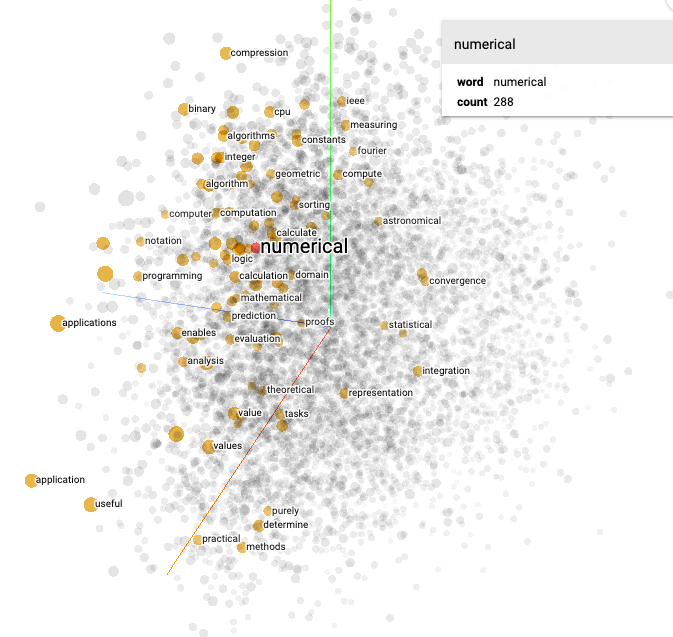
\includegraphics[width=0.65\textwidth]{capitulo2/figuras/an1.png}
	\caption{Representacion vectorial tridimensional de incrustaciones de palabras en TensorBoard}
	\floatfoot{Fuente: Elaboracion propia utilizando TensorBoard }
	\label{fig:tensorboard}
\end{figure}

Uno de los subcampos fundamentales del aprendizaje automático, que depende en gran medida de la calidad y cantidad de los datos, es el aprendizaje profundo. El aprendizaje profundo se centra en el entrenamiento de redes neuronales con múltiples capas apiladas, cada una compuesta por neuronas interconectadas que realizan operaciones matemáticas con los datos.

La diferencia principal entre las redes neuronales tradicionales y las redes neuronales profundas radica en la capacidad de estas últimas para comprender características complejas de los datos. Un ejemplo notable de esta capacidad se evidencia en modelos de aprendizaje profundo como Word2Vec, cuya función es representar palabras como vectores densos.\\
Word2Vec tiene en cuenta el contexto en el que aparecen las palabras, lo que facilita la captura de significados contextualmente relevantes. En la Figura \ref{fig:tensorboard}  se puede observar una representación de embeddings de 10,000 palabras en la interfaz de Tensorflow. Con el vector de la palabra ``numerical'' como punto de referencia, se pueden observar los vectores de las palabras más cercanos a numerical que, resaltan ya sea por contexto, sintaxis o similitud semántica. El cálculo de estas características complejas sólo puede llevarse a cabo mediante redes de aprendizaje profundo. 

Esta breve introducción tiene como objetivo dar una perspectiva amplia sobre estos conceptos fundamentales con algunos ejemplos que permitan comprender las aplicaciones del aprendizaje automático y profundo. En las siguientes secciones del capítulo se realizará una exploración más profunda sobre el funcionamiento, las ventajas y limitaciones de estas dos áreas de estudio.



\section{NEURONAS BIOLÓGICAS VS NEURONAS ARTIFICIALES}
A continuación se presentan trabajos relevantes que han contribuido a la representación de la neurona, sentando las bases de los modelos neuronales actuales. Además, se explora en detalle el funcionamiento y las características de una neurona artificial, tal como se conoce comúnmente en la actualidad.
\subsection{ Modelo neuronal de Warren McCulloch y Walter Pitts}
Uno de los trabajos más relevantes sobre la representación de una neurona biológica fue el de Warren McCulloch y Walter Pitts quienes se consideran  pioneros en el campo de las neurociencias computacionales y la teoría de las redes neuronales artificiales. En 1943, publicaron un artículo titulado ``A Logical Calculus of Ideas Immanent in Nervous Activity'' (``Un cálculo lógico de ideas inmanentes en la actividad nerviosa''), donde presentaron un modelo muy simplificado de una neurona biológica, que es considerado uno de los primeros modelos de neuronas artificiales\cite{mcculloch1943logical}.

\begin{figure}
	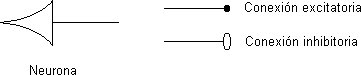
\includegraphics[width=0.65\textwidth]{capitulo2/figuras/an2.png}
	\caption{Representacion grafica de una neurona y sus dos tipos de conexiones}
	\floatfoot{Fuente: El modelo neuronal de McCulloch y Pitts: Interpretacion comparativa del modelo \cite[ p.4]{prieto2020modelo} }
	\label{fig:an2}
\end{figure}

Este modelo propuesto  fue una abstracción matemática de cómo funciona una neurona biológica, y fue formulado como un sistema de lógica binaria. En su modelo, una neurona recibe múltiples señales de entrada (excitatorias o inhibitorias) y produce una única salida binaria basada en una función umbral. Si la suma de las señales de entrada superaba un cierto umbral, la neurona se activaba y emitía una señal de salida, de lo contrario, permanecía inactiva.

\begin{figure}[h!]
	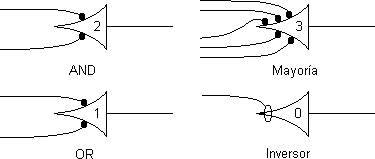
\includegraphics[width=0.65\textwidth]{capitulo2/figuras/an3.png}
	\caption{Algunos ejemplos de la implantacion de funciones logicas}
	\floatfoot{Fuente: El modelo neuronal de McCulloch y Pitts: Interpretacion comparativa del modelo \cite[p. 5]{prieto2020modelo} }
	\label{fig:an3}
\end{figure}

Aunque este modelo es muy simple en comparación con la complejidad de las neuronas biológicas reales, sentó las bases para el desarrollo de redes neuronales artificiales, esto debido a que ellos podían darnos a entender que la resolución de problemas más complejos  podría ser posible con la  conexión de muchas de estas neuronas. En la Figura \ref{fig:an2} se puede observar la representación básica de una neurona interpretando al modelo de Warren McCulloch y Walter Pitts , donde se aborda y representa los conceptos de conexión excitatoria e inhibitoria, que es equivalente a la sinapsis excitatoria e inhibitoria de una neurona biológica. En la Figura \ref{fig:an3} en la esquina superior izquierda se puede observar a la representación de una neurona cuyo funcionamiento es equivalente a una compuerta and de dos entradas, en la esquina inferior izquierda se encuentra otra neurona que es equivalente a una compuerta or de dos entradas , en la esquina superior derecha se aprecia a una neurona or de 5 entradas con un umbral de tres y finalmente en la esquina inferior derecha se observa una neurona con una  conexión inhibitoria con umbral cero.






\subsection{Perceptrón de clasificación binaria}
El perceptrón es un modelo de neurona artificial llamada unidad lógica de umbral (TLU, por sus siglas en inglés: Threshold Logic Unit) , desarrollado por Frank Rosenblatt en 1957. Es un modelo simple, donde una única neurona puede ser utilizada para problemas de clasificación binaria \cite{rosenblatt1957perceptron}.

El perceptrón es un caso particular y simple, con una función de activación específica y aplicable principalmente a problemas lineales. “En el caso del perceptrón, la elección de la función de activación de signo está motivada por el hecho de que es necesario predecir una etiqueta de clase binaria” \cite[p. 11]{aggarwal2018neural}. Esta función de activación suele ser una función escalón, produciendo una salida binaria (0 o 1).  Por lo tanto se utiliza para problemas de clasificación linealmente separables, lo que significa que solo puede resolver problemas donde se puede trazar una línea o un hiperplano para separar claramente las clases en un espacio de características.

\begin{figure}
	
	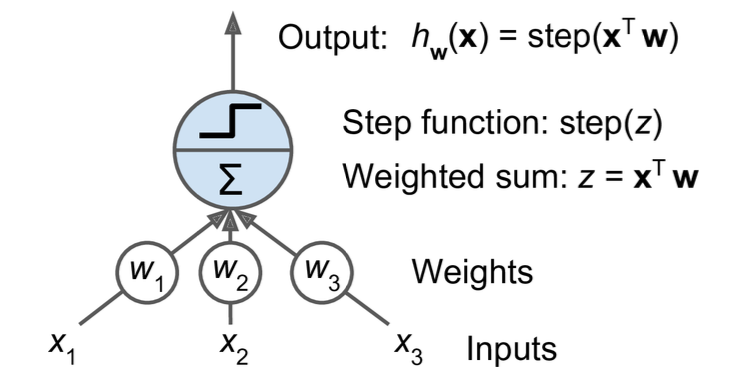
\includegraphics[width=0.65\textwidth]{capitulo2/figuras/an4.png}
	\caption{Unidad logica de umbral \\ \textit{Fuente:Extraido de \protect\cite[p. 282]{geron2019hands}}}
	\label{fig:an4}
\end{figure}

``El TLU calcula una combinación lineal de las entradas ( $\text{z} = w_1x_1 + w_2x_2 + \cdots + w_nx_n = x_Tw$) y si el resultado excede un umbral determinado en la función de paso , genera la clase positiva o genera la clase negativa''\cite[p. 282]{geron2019hands} ver Figura \ref{fig:an4}. 

La representación de una neurona artificial actual puede tener una función de activación más compleja que el escalón,  para permitir el aprendizaje en diferentes contextos. Por ejemplo, se puede emplear una función sigmoidal, tangente hiperbólica, ReLU, entre otras.







\subsection{Representación de una neurona artificial}
La comprensión actual de las neuronas artificiales, fundamentales en las redes neuronales del aprendizaje automático, se origina en la inspiración biológica y en modelos iniciales como los de Warren McCulloch, Walter Pitts y Frank Rosenblat . 

\begin{figure}[h!]
	\centering
	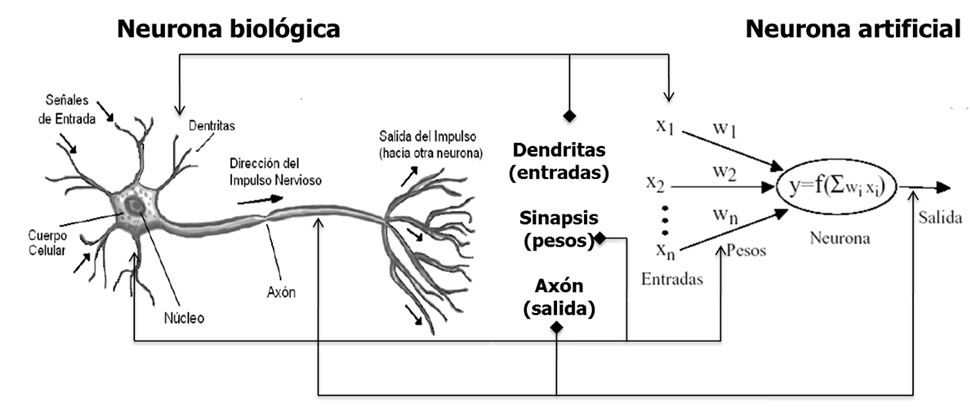
\includegraphics[width=0.65\textwidth]{capitulo2/figuras/an5.png}
	\caption{Comparación entre una neurona biológica y  artificial \\ \textit{Fuente: Extraido de \protect\cite[p. 4]{lao2017procedimiento}}}
	\label{fig:an5}

\end{figure}


El enfoque de McCulloch y Pitts representaba la neurona más  o menos como una compuerta lógica, la representación actual de la neurona en el contexto de las redes neuronales muestra una mayor complejidad y una aproximación más fiel a las funciones y comportamientos observados en el enfoque propuesto por Frank Rosenblatt. Este avance refleja un modelo más detallado y más cercano a la naturaleza multifacética y dinámica de las neuronas biológicas ver Figura \ref{fig:an5}.


Estructura Básica:
\begin{itemize}
	\item	 Neurona biológica: En el cerebro humano, las neuronas son células especializadas que forman la unidad básica del sistema nervioso. Tienen una estructura celular con un cuerpo celular, dendritas, axones y sinapsis.
	\item	Neurona artificial: En informática, una neurona artificial es la unidad básica de una red neuronal. Consiste en entradas, pesos, una función de activación y una salida.
\end{itemize}


Recepción y Transmisión de Señales:
\begin{itemize}
	\item	 Neurona biológica: Las dendritas reciben señales de otras neuronas a través de sinapsis. Cuando se acumula una cantidad suficiente de señales excitatorias o inhibitorias, se genera un impulso eléctrico a lo largo del axón hasta llegar a los botones sinápticos y posteriormente a la siguiente o siguientes neuronas, donde el proceso se repite nuevamente.
	\item	Neurona artificial: Recibe múltiples entradas que son multiplicadas por su respectivo peso, el peso que interviene en las entradas será lo suficientemente grande o pequeño para influir o no en la salida que posteriormente se modificará por alguna función de activación, debido a esta tarea es que la función de sinapsis de una neurona biológica es conceptualmente equivalente a la función de los pesos en una neurona artificial. 
\end{itemize}
Adaptabilidad y Aprendizaje:
\begin{itemize}
	\item	 Neurona biológica: Las neuronas biológicas pueden cambiar su conectividad y fuerza sináptica a lo largo del tiempo, lo que permite el aprendizaje y la adaptabilidad.
	\item	Neurona artificial: Los pesos en las neuronas artificiales pueden ajustarse durante el entrenamiento mediante algoritmos de aprendizaje, lo que permite que la red neuronal aprenda y mejore su capacidad para resolver tareas específicas.
\end{itemize}


\subsection{Función de entrada}
La función de entrada en una neurona artificial es el cálculo ponderado de las señales de entrada que recibe la neurona antes de aplicar una función de activación para producir la salida. En términos simples, la función de entrada representa cómo se combinan y procesan las entradas para determinar la actividad de la neurona.

En una neurona artificial básica, la función de entrada realiza alguna operación matemática conveniente, generalmente la suma de las señales de entrada multiplicadas por sus respectivos pesos. Esta suma ponderada se representa en la ecuación \ref{eq:e1}:

\begin{equation} \label{eq:e1} 
	Entrada = w_1x_1 + w_2x_2 + \cdots + w_nx_n + b 
\end{equation}

Donde : 
\begin{itemize}
\item $w_1, w_2, \ldots, w_n$ son los pesos asociados a cada señal de entrada $x_1, x_2, \ldots, x_n$ respectivamente.
\item $b$ es el sesgo (bias), un parametro adicional que se suma a la suma ponderada
\end{itemize}

\begin{figure}[h!]
	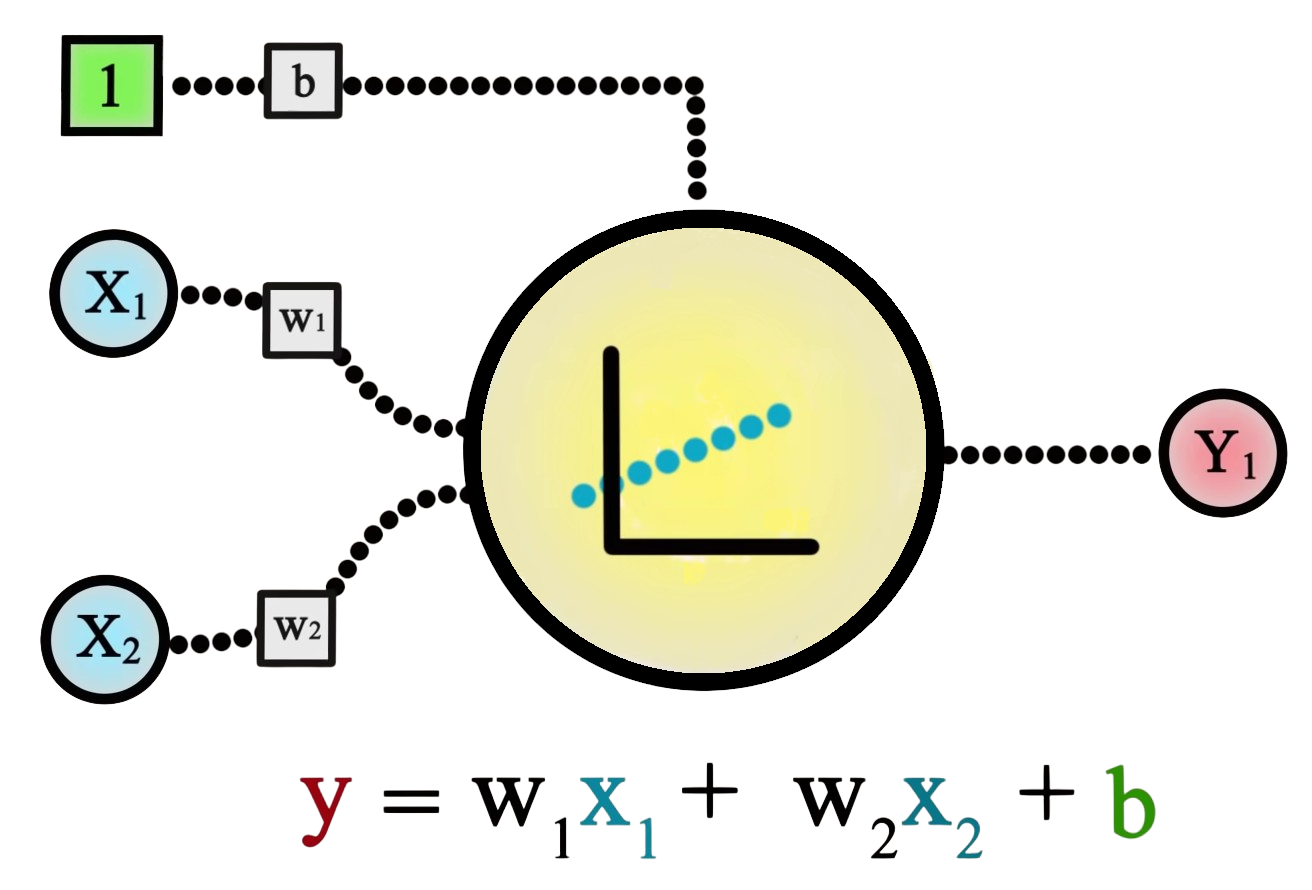
\includegraphics[width=0.65\textwidth]{capitulo2/figuras/an6.png}
	\caption[Representacion de una neurona artificial]{Representacion de una neurona artificial
		\\\textit{Fuente: Elaboracion Propia}}
	\label{fig:an6}
\end{figure}

Los pesos indican la importancia relativa de cada entrada en la determinación de la salida de la neurona, es decir, que permiten que un gran valor de entrada tenga solamente una pequeña influencia, si estos son lo suficientemente pequeños. El sesgo o bias es un término independiente que permite desplazar la función de entrada, lo que puede ser crucial para el aprendizaje y la adaptación de la red neuronal. Ver Figura \ref{fig:an6}. La función de entrada, en esencia, realiza un procesamiento lineal de las entradas ponderadas por sus pesos. Posteriormente, esta suma ponderada se introduce en una función de activación.


\subsection{Función de activación}
La función de activación es una función matemática no lineal que recibe las entradas procesadas de la neurona, se encarga de distorsionar el valor de salida, añadiendo valores no lineales. Ya que la neurona realiza generalmente una suma ponderada de sus entradas y esto puede asemejarse en esencia a un modelo lineal, para tratar problemas que no son solamente lineales se necesitan modelos más complejos, por lo tanto este es el propósito de una función de activación. ``Por ejemplo, si la variable objetivo que se va a predecir es real, entonces tiene sentido utilizar la función de activación de identidad y el algoritmo resultante es el mismo que el de la regresión de mínimos cuadrados.'' \cite[p. 11]{aggarwal2018neural}. Las funciones de activación más comúnmente utilizadas se detallan a continuación:


Función identidad: Es una función lineal que conserva el valor de entrada como salida, es la función más básica ya que no proporciona no linealidad:  Ver ecuación \ref{eq:e2}

\begin{equation} \label{eq:e2} 
	f(x) = x 
\end{equation}


	
Función sigmoide: Esta función tiene una forma de ``S'' y transforma la entrada a un rango de valores entre 0 y 1, esta característica facilita la interpretación como probabilidades, se alinea bien con modelos de máxima verosimilitud y permite la construcción de funciones de pérdida adecuadas para problemas de clasificación. Ver ecuación \ref{eq:e3}

\begin{equation} \label{eq:e3} 
	sigmoide(t)=\frac{1}{1+e^{-t}}
\end{equation}

 
	
	
Función tangente hiperbólica: Similar a la función sigmoide, pero tiene un rango entre -1 y 1. Es preferible a la sigmoide cuando se desea que los resultados de los cálculos sean tanto positivos como negativos. Su fórmula directa se puede observar en la ecuación \ref{eq:e4}.
 

\begin{equation} \label{eq:e4} 
tanh(x) = \frac{e^{x}-e^{-x}}{e^{x}+e^{-x}}
\end{equation}
	
Función tangente hiperbólica dura: La función ``hard tanh'' es una variante de la función tangente hiperbólica (tanh) que ha sido modificada para producir salidas en un rango limitado y discretizado, manteniendo las propiedades no lineales de la función tanh original pero restringiendo su rango de salida.
La función ``hard tanh'' es similar a la función tangente hiperbólica estándar, pero en lugar de proporcionar salidas en el rango continuo entre -1 y 1, aplica un límite a los valores de salida.

\begin{equation} \label{eq:e5} 
	hardTanh(x)=max(min(x,1), -1)
\end{equation}

	
	
Función ReLu: La función rectificada lineal se comporta de manera constante cuando el valor de z es menor a cero, o como una función lineal cuando el valor de z es mayor o igual a cero. ver ecuación \ref{eq:e6}

\begin{equation} \label{eq:e6} 
	relu(z)=max(0,z)
\end{equation}


Función softmax: Esta función transforma las salidas a una representación en forma de probabilidades, de tal manera que el sumatorio de todas las probabilidades de las salidas de uno. ver ecuación \ref{eq:e7}
\begin{equation} \label{eq:e7} 
	softmax(z_{j})=\frac{e^{z_{j}}}{\displaystyle\sum_{k=1}^{K}e^{z_{k}}}
\end{equation}




\subsection{ Función de salida}
La función de salida en una neurona artificial es la función que determina la salida final o el resultado de la neurona después de procesar las entradas y aplicar la función de activación. Esta función determina qué valor se transfiere a las neuronas vinculadas. ``Si la función de activación está por debajo de un umbral determinado, ninguna salida se pasa a la neurona subsiguiente.''\cite[p. 12]{matich2001redes} Normalmente, no cualquier valor es permitido como una entrada para una neurona. Algunos de los valores de salida pueden ser la salida misma o también pueden ser binarios {0, 1} o {-1, 1}.
\section{REDES NEURONALES}
En esta sección se detalla con más profundidad  acerca de los diversos conceptos de funcionamiento y arquitectura de redes neuronales.

\subsection{Redes neuronales feedforward}
Las redes neuronales feedforward, presentan una arquitectura donde la información fluye en una dirección única, avanzando desde la capa de entrada a través de una serie de capas ocultas hasta llegar a la capa de salida, sin ciclos ni retroalimentación. Por ejemplo, podemos visualizar este flujo como una sucesión de funciones $f_1(), f_2(), y f_3()$ encadenadas para formar $f(x) = f_3(f_2(f_1(x)))$. Estas estructuras en cadena son las formas más comunes de redes neuronales.

En esta secuencia, $f_1()$ representa la primera capa de la red, $f_2()$ sería la segunda capa, y así sucesivamente. La extensión total de esta cadena determina la profundidad del modelo. Este concepto de profundidad es esencial en la terminología del ``aprendizaje profundo'', un nombre derivado precisamente de esta característica.

Este enfoque, descrito en el libro Deep Learning \cite[p.167]{goodfellow2016deep}, permite representar y procesar datos de manera más compleja, ya que cada capa sucesiva puede aprender y extraer características más abstractas de los datos de entrada, posibilitando así la resolución de problemas complejos.

\subsection{Perceptrón multicapa}
El perceptrón multicapa, también conocido como red neuronal de múltiples capas es un ejemplo de red neuronal profunda feedforward, es una extensión del perceptrón simple que consta de múltiples capas de neuronas interconectadas, la representación gráfica de un perceptron multicapa con dos capas ocultas se puede observar en la figura \ref{fig:an7}. A diferencia del perceptrón de una sola capa, el perceptrón multicapa tiene al menos una capa oculta (capas entre la capa de entrada y la capa de salida), lo que le permite resolver problemas más complejos y no linealmente separables.

Esta red neuronal se entrena utilizando algoritmos de aprendizaje supervisado, como retropropagación (backpropagation), que ajustan los pesos de las conexiones entre las neuronas para minimizar una función de pérdida, mejorando así la capacidad de la red para hacer predicciones precisas.

\begin{figure}[h!]
	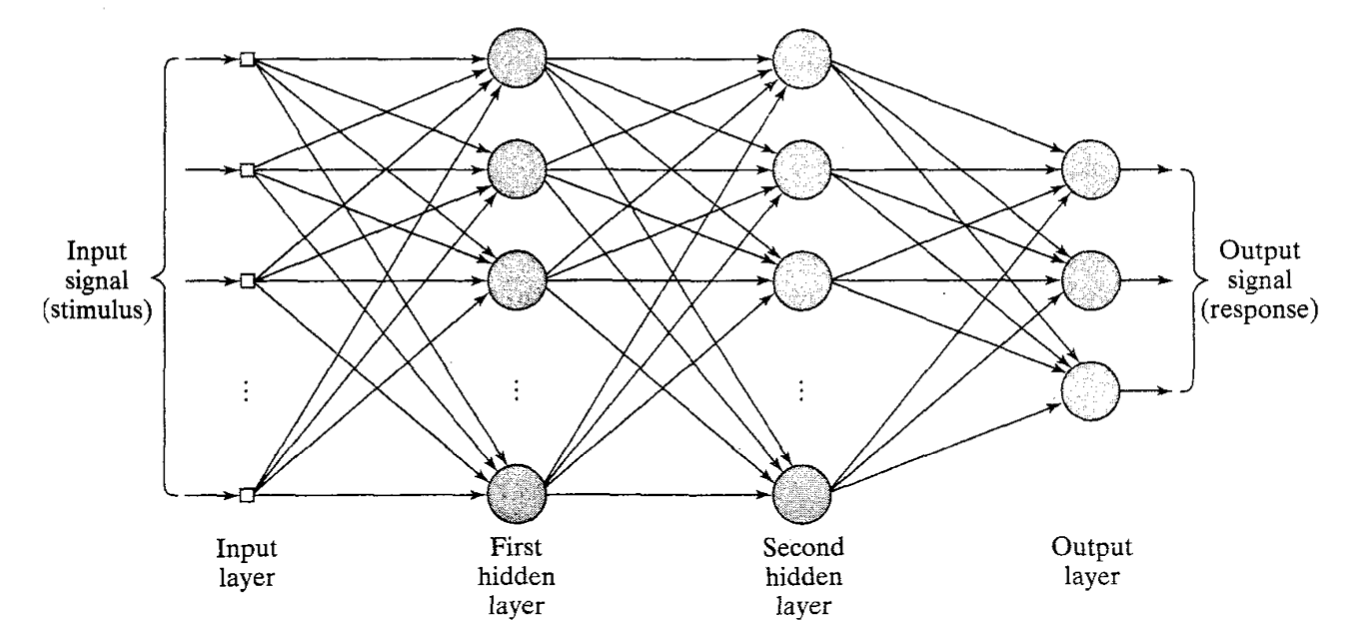
\includegraphics[width=0.65\textwidth]{capitulo2/figuras/an7.png}
	\caption[Grafo arquitectonico de un perceptron multicapa con dos capas ocultas]{Grafo arquitectonico de un perceptron multicapa con dos capas ocultas
		\\\textit{Fuente: Extraído de} \protect\cite[p.281]{haykin1998neural}}
	\label{fig:an7}
\end{figure}

El perceptrón multicapa es una red neuronal típica, puede constar de varias capas y conexiones entre neuronas. Su arquitectura detallada en la figura \ref{fig:an7} sigue la estructura básica de cualquier red neuronal profunda, la misma consta de los siguientes elementos: 
\begin{itemize}

	\item Capa de Entrada: 
	
	Esta capa recibe los datos brutos o características de entrada. Cada neurona en esta capa representa una característica o variable de entrada.

	\item Capas Ocultas: 
	
	Las capas ocultas (una o varias) entre la capa de entrada y la capa de salida procesan los datos y extraen características significativas de manera no lineal. Cada neurona en una capa oculta toma las salidas de la capa anterior como entrada, realiza cálculos y transfiere la salida a la siguiente capa.

	\item Capa de Salida:
	
	Esta capa produce la salida final de la red neuronal. La cantidad de neuronas en esta capa depende del tipo de problema que se esté abordando. Por ejemplo, en un problema de clasificación binaria, podría tener una neurona que produzca una salida entre 0 y 1. En problemas de clasificación multiclase, habría tantas neuronas de salida como clases a predecir, cada una representando la probabilidad de pertenencia a esa clase.
\end{itemize}
\section{APRENDIZAJE AUTOMÁTICO SUPERVISADO}
El aprendizaje automático supervisado, es un enfoque dentro del campo del aprendizaje automático, donde se entrena un modelo utilizando un conjunto de datos etiquetados. En este método, el modelo se entrena para aprender la relación entre las características (variables independientes) y las etiquetas o salidas deseadas (variables dependientes) presentes en los datos de entrenamiento. Como se puede apreciar en la Figura \ref{fig:an8}, donde el conjunto de entrenamiento consiste en mensajes de correo etiquetados como spam o no spam, a partir del cual el modelo podrá predecir a cuál de las dos clases corresponde algún otro correo no etiquetado (nueva instancia). 

\begin{figure}
	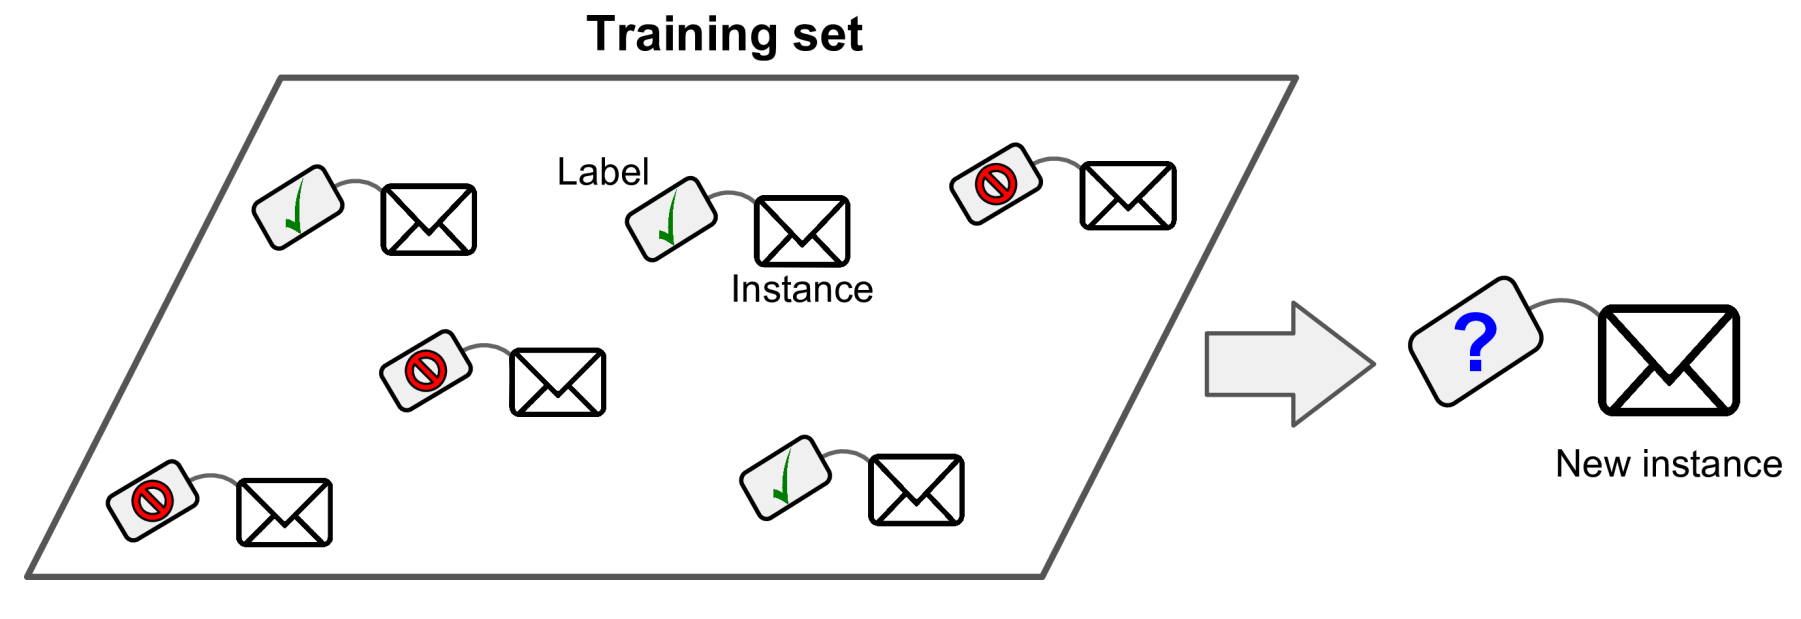
\includegraphics[width=0.65\textwidth]{capitulo2/figuras/an8.png}
	\caption{Un conjunto de entrenamiento etiquetado para aprendizaje supervisado}
	\floatfoot{Fuente: Hands-on machine learning with Scikit-Learn, Keras, and TensorFlow \cite[p. 8]{geron2019hands} }
	\label{fig:an8}
\end{figure}
\subsection{Entrenamiento}
El aprendizaje en una red neuronal supervisada se logra a través de su entrenamiento. Como se mencionó previamente, este proceso implica la adaptación de los pesos y sesgos de las conexiones entre las neuronas para permitir al modelo realizar predicciones precisas sobre nuevos datos. Este proceso se divide en varias fases esenciales que pueden agruparse de la siguiente manera:

\textbf{Propagación hacia adelante}

Una vez que se ha definido la arquitectura de una red neuronal con su cantidad de capas, neuronas por capa, y funciones de activación, el siguiente paso es la inicialización de los pesos. Los pesos y sesgos de la red neuronal pueden ser asignados aleatoriamente o con valores predefinidos.
Lo que sigue es realizar la Propagación hacia Adelante (Forward Propagation) a través de toda la red, este proceso implica el paso de los datos de entrada a través de la red neuronal, capa por capa, desde la capa de entrada hasta la capa de salida, para generar una predicción o salida. Durante esta fase, cada capa de la red neuronal realiza dos operaciones clave:

\begin{itemize}
	\item Ponderación y Suma: Cada neurona en una capa recibe entradas de todas las neuronas de la capa anterior, multiplicadas por los pesos respectivos. Estos productos se suman junto con el sesgo asociado a la neurona. Esta operación puede representarse como $Z=W\cdot X+b$, donde $Z$ almacena el valor de la suma ponderada.
	\item Activación: Después de la suma ponderada, se aplica la función de activación determinada para cada capa a la salida resultante . Esta función introduce no linealidad en la red, permitiendo aprender relaciones y patrones complejos en los datos. Si representamos la función de activación como $A()$, hasta este punto, el proceso realizado sería $A(Z)$, es decir, la suma ponderada pasó por la función de activación. ``Esto da como resultado una cascada directa de cálculos entre las capas, utilizando el conjunto actual de pesos. La salida final prevista se puede comparar con la de la instancia de entrenamiento y se calcula la derivada de la función de pérdida con respecto a la salida.''\cite[p.22]{aggarwal2018neural}.
\end{itemize}

La propagación hacia adelante se utiliza tanto en el entrenamiento como en la predicción de una red neuronal. Durante el entrenamiento, se utiliza para generar predicciones con los datos de entrenamiento y calcular la pérdida, que luego se utiliza en el proceso de retropropagación para ajustar los pesos y mejorar las predicciones. En la predicción o evaluación de nuevos datos, la red simplemente realiza la propagación hacia adelante para generar predicciones sin actualizar los pesos de la red.


\textbf{Propagación hacia atrás}

La retropropagación (backpropagation) en el entrenamiento de redes neuronales ajusta tanto los pesos como los sesgos. Durante el proceso de retropropagación, se calculan los gradientes de la función de coste respecto a todos los pesos y sesgos en la red.

Estos gradientes (derivadas parciales) indican la dirección y la magnitud en la que se debe ajustar cada peso y cada sesgo para minimizar la función de coste. Posteriormente, se utilizan estos gradientes en algoritmos de optimización, como el descenso del gradiente, para actualizar tanto los pesos como los sesgos en la red con el objetivo de mejorar el rendimiento del modelo. Para esto debemos tomar en cuenta los siguientes procedimientos y cálculos a realizar:

\begin{itemize}
	\item Pérdida
	
Una vez que se realiza la primera fase de entrenamiento, obtendremos  la salida correspondiente de la red neuronal, se procederá a calcular la pérdida. La pérdida se calcula con la función de coste, también conocida como función de pérdida, es una métrica que cuantifica qué tan bien está realizando un modelo de aprendizaje automático sus predicciones, al compararlas con las salidas reales o etiquetas conocidas en un conjunto de datos de entrenamiento. 
	\item Función de coste
	
La función de coste, representada como $(C())$, evalúa la discrepancia entre las predicciones del modelo y las salidas esperadas. Esta métrica genera un único valor numérico que indica qué tan distantes se encuentran las predicciones del modelo respecto a las salidas reales. El objetivo primordial es minimizar esta función de coste durante el proceso de entrenamiento con el fin de mejorar las predicciones del modelo.
	
Diversas funciones de coste se emplean según el tipo de problema que se enfrenta. Por ejemplo, en problemas de regresión se utilizan funciones de coste comunes como el error cuadrático medio (mean squared error), el error absoluto medio, el error cuadrático medio logarítmico, entre otros. Para problemas de clasificación, se recurre a la función de pérdida bisagra (hinge loss) en modelos como SVM, y la pérdida focal (focal loss), diseñada para abordar desequilibrios en la distribución de clases.

La selección de la función de coste siempre está ligada al tipo de salida y al problema específico que se está abordando. En todos los casos, existen funciones de coste diseñadas para adaptarse y optimizarse según las necesidades particulares. Por ejemplo, la entropía cruzada suma sobre todas las clases y evalúa la discrepancia entre las distribuciones de probabilidad reales y las predichas para cada clase.
El término $log(y_{i})$ dentro de la entropía cruzada penaliza de manera significativa las predicciones incorrectas o poco confiables. Esta penalización aumenta conforme la predicción se aleja más del valor real. Ver ecuación \ref{eq:e8}

\begin{equation} \label{eq:e8} 
	L(y,{y}')=-\displaystyle\sum_{i=1}^{n}y_{i}log(y_{i}')
\end{equation}


$\sum_{i=1}^{n} =$ sumatoria de todos los valores\\
$y_{i} =$ etiqueta real para la clase i\\
$y_{i}' =$ predicción del modelo para la clase i\\

Esta función de coste se emplea principalmente en problemas de clasificación, abarcando variantes como la entropía cruzada binaria (Binary Cross-Entropy) y la entropía cruzada categórica (Categorical Cross-Entropy).

	\item Vector gradiente
	
	
El siguiente paso implica encontrar las derivadas parciales de todos los parámetros $(w, b)$ de la red neuronal en relación con la función de coste. Este proceso permitirá optimizar la red neuronal utilizando el algoritmo del descenso del gradiente. Para ello, se debe calcular el vector gradiente, el cual consta de las derivadas del costo respecto al peso $\frac{\partial C}{\partial W}$ y las derivadas del costo respecto al sesgo $\frac{\partial C}{\partial b}$.

Hasta este punto, la suma ponderada de cada neurona ha pasado por su respectiva función de activación y finalmente por la función de coste seleccionada, expresada como $C(A(Z))$. Este proceso, donde el resultado de una función se pasa por otra y luego por otra más, se conoce como composición de funciones. Para calcular la derivada de una composición de funciones, se emplea la regla de la cadena (chain rule). Esta regla indica que para encontrar la derivada de una composición de funciones, simplemente se multiplican las derivadas intermedias de cada una. Por ejemplo:

Se tiene dos funciones : $x= h(a) , y= j(c)$

Si existe una relación entre $x$ y $c$ (por ejemplo, $x=2c$), se crea una composición de funciones $x=h(j(c))$, donde $x$ depende de $c$ a través de la función $j$ y luego de $h$.
La regla de la cadena establece que si se tiene una composición de funciones como $x=h(j(c))$, su derivada $\frac{dx}{dc}$ se calcula multiplicando las derivadas de cada función individual.
Es decir, esta derivada es el producto de las derivadas de cada función individual: $\frac{dx}{dc} = \frac{dx}{da} \cdot \frac{da}{dc}$

Por lo tanto hallar la derivada del peso respecto al costo y la derivada del bias respecto al costo de la última capa de la red neuronal equivale a las ecuaciones \ref{eq:e9} y \ref{eq:e10}.
\begin{equation} \label{eq:e9} 
	\frac{\partial C}{\partial W^L}=\frac{\partial C}{\partial A^L}\cdot \frac{\partial A^L }{\partial Z^L}\cdot \frac{\partial Z^L }{\partial W^L}
\end{equation}

\begin{equation} \label{eq:e10} 
	\frac{\partial C}{\partial b^L}=\frac{\partial C}{\partial A^L}\cdot \frac{\partial A^L }{\partial Z^L}\cdot \frac{\partial Z^L }{\partial b^L}
\end{equation}

$\frac{\partial C}{\partial W^L} $.- Representa la derivada parcial de la función de coste C respecto a un peso específico W. Esta derivada indica cómo cambia la función de coste C cuando se modifica un peso particular W en la red.

$\frac{\partial C}{\partial A^L} $.- Es la derivada parcial del coste  respecto a la activación , indica cómo cambia la función de costo C en función de los cambios en la activación A en la última capa L de la red neuronal.

$\frac{\partial A^L }{\partial Z^L} $.- Representa la derivada parcial de la activación A respecto a la suma ponderada Z. Indica cómo pequeños cambios en la suma ponderada Z afectarán la activación A.

$\frac{\partial Z^L }{\partial W^L} $.- Representa la derivada parcial de la suma ponderada Z respecto a un peso particular W, indica como la suma ponderada Z, cambia con respecto a cada peso específico W.

$\frac{\partial C}{\partial b^L} $.- Representa la derivada parcial de la función de coste C respecto al sesgo b. Esta derivada indica cómo cambia la función de coste C cuando se modifica el sesgo b en la red.

$\frac{\partial Z^L }{\partial b^L} $.- Representa la derivada parcial de la suma ponderada Z respecto al sesgo b indica cómo pequeños cambios en el sesgo b afectarán la suma ponderada Z. Sin embargo, es importante tener en cuenta que, la derivada de Z respecto a b generalmente es 1, ya que el sesgo se suma directamente a la suma ponderada Z sin multiplicaciones adicionales.

El cálculo que se realizó hasta ahora es aplicable solamente para la última capa de la red neuronal. La ecuación \ref{eq:e11} y la ecuación \ref{eq:e12} representan las derivadas parciales para la capa $L-1$, es decir la penúltima capa. Estas ecuaciones también son aplicables para todas las capas anteriores. En esta caso  importante notar que las derivadas del coste respecto a la activación $\partial  A^L$  y la derivada de la activación respecto a la suma ponderada  $\frac{\partial  A^L}{\partial  Z^L}$ ya calculadas en la última capa, serán reutilizadas.  Este proceso se repetirá hasta terminar con el cálculo hacia atrás de todas las capas.
\begin{equation} \label{eq:e11} 
	\frac{\partial C}{\partial W^{L-1}}=\frac{\partial C}{\partial A^L}\cdot \frac{\partial A^L }{\partial Z^L}\cdot \frac{\partial Z^L }{\partial A^{L-1}}\cdot \frac{\partial A^{L-1} }{\partial Z^{L-1}}\cdot \frac{\partial Z^{L-1}}{\partial W^{L-1}}
\end{equation}

\begin{equation} \label{eq:e12} 
	\frac{\partial C}{\partial b^{L-1}}=\frac{\partial C}{\partial A^L}\cdot \frac{\partial A^L }{\partial Z^L}\cdot \frac{\partial Z^L }{\partial A^{L-1}}\cdot \frac{\partial A^{L-1} }{\partial Z^{L-1}}\cdot \frac{\partial Z^{L-1}}{\partial b^{L-1}}
\end{equation}


	\item Descenso del gradiente
	
El descenso del gradiente es un algoritmo de optimización cuyo objetivo principal es encontrar el mínimo de una función de coste o pérdida. La idea detrás del descenso del gradiente es iterativamente actualizar los parámetros del modelo (pesos y sesgos ) en la dirección y la magnitud que reduce gradualmente la función de coste. Esto se logra siguiendo el vector del gradiente de la función de coste con respecto a esos parámetros. El gradiente indica la dirección hacia el máximo crecimiento de la función de coste; por lo tanto, avanzar en dirección opuesta al gradiente nos lleva hacia un mínimo local (o global) de la función no convexa. La actualización de los parámetros $\theta$ (pesos, sesgos, etc.) se realiza utilizando la fórmula que se muestra en la ecuación \ref{eq:e13}.
\begin{equation} \label{eq:e13} 
	\theta = \theta - \alpha \cdot\triangledown J(\theta)
\end{equation}


Donde:

$\theta$ son los parámetros del modelo.

$\alpha$  es la tasa de aprendizaje (learning rate), es un valor pequeño que controla la velocidad a la que se actualizan los parámetros.

$\triangledown J(\theta)$  es el gradiente de la función de coste.

El proceso implica utilizar el gradiente de la función de coste con respecto a cada parámetro, y luego ajustar los parámetros en pequeños pasos proporcionales a este gradiente multiplicado por una tasa de aprendizaje (learning rate). Esta tasa de aprendizaje determina la longitud de cada paso que damos hacia el mínimo.

El descenso del gradiente puede tener diferentes variantes, como el descenso del gradiente estocástico (SGD), el descenso del gradiente por lotes (Batch Gradient Descent), el descenso del gradiente en lotes pequeños (Mini Batch Gradient Descent), entre otros, que varían en la cantidad de datos utilizados para cada actualización de los parámetros y la manera en que se actualizan estos parámetros.

\end{itemize}

\subsection{Sobreajuste y Subajuste}
Se detallarán dos conceptos muy importantes que se deben tener en cuenta al momento de examinar el rendimiento de un modelo de aprendizaje automático

\begin{itemize}
\item{Sobreajuste}
\end{itemize}


El sobreajuste (overfitting) es un fenómeno en el aprendizaje automático donde un modelo se ajusta demasiado a los datos de entrenamiento. Esto significa que el modelo aprende no solo los patrones generales presentes en los datos, sino también el ruido o las particularidades específicas de esos datos de entrenamiento. Como resultado, el modelo puede tener un excelente rendimiento en los datos utilizados para entrenarlo pero se desempeña mal al enfrentarse a nuevos datos (conjunto de datos de validación o prueba) que no ha visto antes. Las causas comunes del sobreajuste incluyen:

\begin{itemize}

	\item Modelo demasiado complejo: Un modelo con una capacidad muy alta puede memorizar los datos de entrenamiento en lugar de aprender patrones generales, lo que conduce a un rendimiento deficiente en datos no vistos.
	
	\item Falta de datos: Cuando hay pocos datos disponibles para el entrenamiento, es más probable que el modelo memorice el ruido presente en esos pocos datos en lugar de aprender patrones generales. .``Esta situación es casi similar al aprendizaje de memoria, que es altamente predictivo para los datos de entrenamiento pero no predictivo para los datos de prueba no vistos''\cite[p. 25]{aggarwal2018neural}.
	
	\item Entrenamiento excesivo: Realizar demasiadas iteraciones o épocas de entrenamiento puede llevar a que el modelo se ajuste demasiado a los datos de entrenamiento, perdiendo la capacidad de generalizar.

\end{itemize}

Para evitar el sobreajuste, se pueden utilizar técnicas como la regularización (L1, L2), validación cruzada, reducción de la complejidad del modelo, aumentó de datos, entre otras estrategias.``Una buena regla general es que la cantidad total de puntos de datos de entrenamiento debe ser al menos 2 o 3 veces mayor que la cantidad de parámetros en la red neuronal, aunque la cantidad precisa de instancias de datos depende del modelo específico en cuestión.''\cite[p. 25]{aggarwal2018neural}. Estas técnicas están diseñadas para reducir la capacidad del modelo de ajustarse excesivamente a los datos de entrenamiento y mejorar su capacidad para generalizar a datos no vistos.

\begin{itemize}
\item{Subajuste}
\end{itemize}


El subajuste (underfitting) es un problema en el aprendizaje automático que ocurre cuando un modelo es demasiado simple para capturar la complejidad de los datos. En este caso, el modelo no puede aprender adecuadamente los patrones presentes en los datos de entrenamiento ni en los datos nuevos. Las causas comunes del subajuste incluyen:

\begin{itemize}

	\item Modelo demasiado simple o poca capacidad: Un modelo simple, con pocos parámetros o capas, puede no ser lo suficientemente flexible como para capturar la complejidad de los datos.
	
	\item Falta de características relevantes: Si el conjunto de datos carece de características informativas o si se eliminan características importantes durante el preprocesamiento, el modelo puede ser incapaz de aprender los patrones relevantes.
	
	\item Entrenamiento insuficiente: No entrenar el modelo durante suficientes iteraciones o épocas puede conducir a que el modelo no logre ajustarse adecuadamente a los datos.
	
\end{itemize}

Para abordar el subajuste, se pueden utilizar estrategias como aumentar la complejidad del modelo (añadiendo capas, neuronas, etc.), ajustar los hiperparámetros, mejorar la calidad de los datos o incluso modificar el enfoque del problema. Estas estrategias buscan proporcionar al modelo la capacidad necesaria para aprender patrones más complejos y, por lo tanto, mejorar su rendimiento en los datos de entrenamiento y en la generalización a nuevos datos.

	
\section{REGULARIZACIÓN}
La regularización es una técnica utilizada en el aprendizaje automático para reducir el sobreajuste en modelos, especialmente en aquellos que son propensos a ajustarse demasiado a los datos de entrenamiento.
El objetivo principal de la regularización es agregar cierta penalización a la función de coste o pérdida del modelo para desalentar la complejidad excesiva y, en su lugar, promover modelos más simples que puedan generalizar mejor a datos no vistos. A continuación se detalla métodos de regularización comunes:

\begin{itemize}
	\item L1 (Regularización Lasso): Esta técnica es una versión regularizada de la regresión lineal, se agrega el término de penalización a la función de coste, mismo que  es equivalente a la suma de los valores absolutos de los pesos. Esto puede llevar a algunos pesos a volverse exactamente cero, lo que puede ser útil para la selección automática de características. ``Una característica importante de Lasso Regression es que tiende a eliminar completamente los pesos de las características menos importantes (es decir, establecerlos en cero).''\cite[p. 140]{geron2019hands}. En la ecuación \ref{eq:e14} se observa  El MSE regularizado con L1.
	
	\item L2 (Regularización Ridge): Esta técnica, tiene el efecto de reducir la magnitud de los coeficientes de los parámetros, penalizando los valores grandes y favoreciendo coeficientes más pequeños. Esto ayuda a prevenir el sobreajuste al evitar que los coeficientes crezcan demasiado para adaptarse únicamente a los datos de entrenamiento, es equivalente a la suma de los cuadrados de los pesos. Esto evita que los pesos tomen valores extremadamente grandes y, por lo tanto, controla la complejidad del modelo. ``La regresión de cresta (también llamada regularización de Tikhonov) es una versión regularizada de la regresión lineal: se agrega un término de regularización igual a $ \alpha\sum_{i=1}^{n}  \theta_i^2$ a la función de costo.''\cite[p. 137]{geron2019hands}. En la ecuación \ref{eq:e15} se observa el MSE regularizado con L2
	
\begin{equation} \label{eq:e14} 
	J(\theta) = \text{MSE}(\theta) + \alpha\sum_{i=1}^{n} \left |  \theta_i \right |
\end{equation}

\begin{equation} \label{eq:e15} 
	J(\theta) = \text{MSE}(\theta) + \alpha\frac{1}{2}\sum_{i=1}^{n} \theta_i^2 
\end{equation}									
				
Donde: 
		
		$\alpha $: Es el hiperparámetro de regularización, es decir controla cuánto se desea regularizar el modelo.\\
		$\sum_{i=1}^{n} \left |  \theta_i \right | $:  es la suma de los valores absolutos de los de los parámetros del modelo.\\
		$\sum_{i=1}^{n} \theta_i^2 $: es la suma de los cuadrados de los parámetros del modelo.\\
		
	\item Dropout: Durante el entrenamiento, aleatoriamente se ``apaga'' un conjunto de unidades/neuronas, lo que fuerza a la red a aprender de manera más robusta al evitar la dependencia excesiva de ciertas neuronas.
	
	\item Early Stopping:  La técnica de parada anticipada(early stopping) detiene el entrenamiento de la red antes de que empiece a sobreajustarse. Se basa en monitorear la precisión en un conjunto de validación y detener el entrenamiento cuando la precisión en este conjunto deja de mejorar. ``Una forma muy diferente de regularizar algoritmos de aprendizaje iterativo como el descenso del grandiente es detener el entrenamiento tan pronto como el error de validación alcance un mínimo. A esto se le llama parada anticipada.''\cite[p. 142]{geron2019hands}.
	
\end{itemize}
\section{REDES NEURONALES CONVOLUCIONALES}
Una red neuronal convolucional (CNN) es un tipo de red neuronal artificial que se distingue por incluir una o más capas convolucionales, donde se realiza la operación matemática de convolución. Este tipo de red ha encontrado una amplia aplicación en el campo de la visión artificial. Surgidas de los estudios sobre la corteza visual del cerebro, estas redes han demostrado un éxito notable en el reconocimiento de imágenes.


A pesar de su origen vinculado principalmente al procesamiento visual, las CNN también han mostrado efectividad en la clasificación de documentos. Según \cite{goldberg2016primer} en A Primer on Neural Network Models for Natural Language Processing, las redes neuronales convolucionales son eficaces en la clasificación de documentos porque tienen la capacidad de identificar características sobresalientes (como tokens o secuencias de tokens). Esto resulta útil para tareas de clasificación donde se espera encontrar pistas locales sólidas sobre la pertenencia a una clase, independientemente de que estas pistas puedan presentarse en diversas partes de la entrada. En la Figura \ref{fig:an9} se puede apreciar a una red neuronal convolucional con una matriz bidimensional de tamaño 7x5 donde cada fila representa a cada elemento en la oración de entrada, la tarea de esta red convolucional es extraer frases útiles para realizar una clasificación binaria que indique el sentimiento de la oración de un fragmento de texto.
\begin{figure}[h!]
	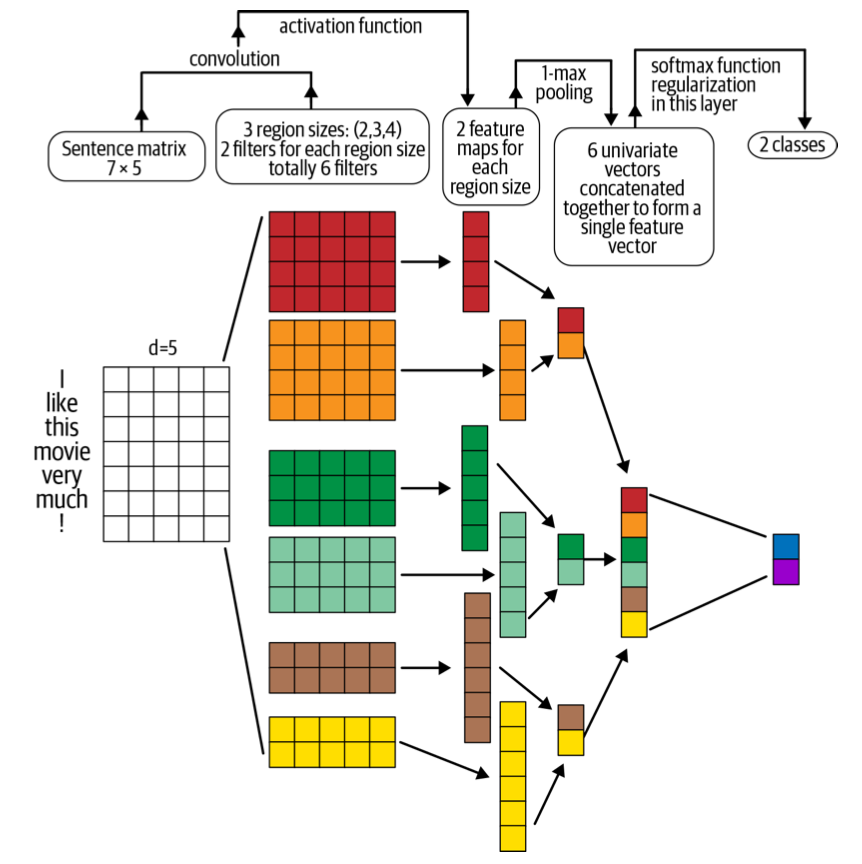
\includegraphics[width=0.6\textwidth]{capitulo2/figuras/an9.png}
	\caption[Modelo CNN en accion]{Modelo CNN en accion
		\\\textit{Fuente: Extraído de} \protect\cite[p. 25]{vajjala2020practical}}
	\label{fig:an9}
\end{figure}

La arquitectura básica de una CNN incluye capas de convolución, las cuales aplican filtros para extraer rasgos relevantes de la entrada. También se incorporan capas de agrupación (pooling) para reducir el tamaño de las representaciones, manteniendo las características más importantes. Por último, las capas totalmente conectadas se encargan de la clasificación final, basándose en los rasgos extraídos por las capas anteriores. Esta arquitectura básica se modifica para adaptarse al procesamiento y clasificación de texto.


\subsection{Breve historia}
Las raíces de las redes neuronales convolucionales (CNN, por sus siglas en inglés Convolutional Neural Networks) se remontan a la década de 1950, cuando entre 1958 y 1959 David Hubel y Torsten Wiesel investigaron la corteza visual realizando experimentos en  gatos. Sus estudios revelaron que muchas de las neuronas en esta región cerebral, tienen pequeños  campos  receptivos locales que reaccionan solamente a estímulos visuales,  ubicados en una región limitada del campo visual.\cite{hubel1959single} Además algunas de estas neuronas  reaccionaban solamente a imágenes con líneas verticales y algunas otras a líneas con distintas orientaciones sin importar que, tuviesen el mismo campo receptivo.  Las neuronas que poseian un campo receptivo más grande, podían reaccionar a patrones más complejos, que eran la combinación de  patrones más simples de un nivel inferior. Este tipo de comportamiento,  hizo que se concluyera a la idea de que las neuronas de nivel superior, se basan en las salidas de las neuronas vecinas de nivel inferior. \cite{hubel1959receptive}

Este trabajo meritorio del Premio Nobel de Fisiología o Medicina inspiró a Fukushima, quien en la década de 1980 propuso la primera arquitectura de red neuronal convolucional conocida como ``Neocognitron''. Este modelo fue capaz de reconocer patrones visuales y estaba compuesto por cuatro tipos de capas entre las cuales resaltaban dos: las capas S (submuestreo) reducían la dimensionalidad de la entrada al tomar secciones de una imagen y reducir su tamaño, preservando las características más relevantes. Las capas C (convolución) eran  responsables de aplicar operaciones de convolución a las entradas. En estas capas, cada neurona estaba conectada únicamente a un área local de las capas previas, reflejando la organización de los campos receptivos locales en las células visuales  \cite{fukushima1980neocognitron}. 

A pesar de estos avances, las CNN no recibieron mayor atención y aplicación práctica hasta la década de 1990, especialmente en el ámbito del reconocimiento de patrones e imágenes. Es en esta época cuando comienzan a destacar y a encontrar aplicaciones prácticas significativas.

El punto de inflexión llegó en 1998, cuando Yann LeCun, junto con otros investigadores, desarrolló una CNN conocida como LeNet-5 para el reconocimiento de dígitos escritos a mano. LeNet-5 fue especialmente revolucionaria porque demostró una alta precisión en la clasificación de dígitos en documentos de cheques bancarios \cite{lecun1998gradient}.

A lo largo de los años, la capacidad de las CNN para procesar datos de imagen se vio fortalecida por la disponibilidad de grandes conjuntos de datos etiquetados, mejoras en hardware (como GPUs) que aceleraron los cálculos intensivos y avances en técnicas de entrenamiento como el uso de funciones de activación no lineales (ReLU) y regularización.

El avance más reciente y significativo de las CNN se produjo con la participación en competiciones de reconocimiento de imágenes, como ImageNet, donde en 2012, un equipo dirigido por Geoffrey Hinton utilizó una CNN denominada ``AlexNet'', que superó ampliamente a otros métodos existentes y estableció un nuevo estándar en el campo de la visión por computadora \cite{krizhevsky2012imagenet}. Desde entonces, las CNN han sido fundamentales en numerosas aplicaciones de reconocimiento de imágenes, segmentación, detección de objetos, entre otros, y continúan siendo objeto de investigación para mejorar su rendimiento y aplicabilidad en una variedad de tareas.

\subsection{Capa de convolución}
La capa de convolución es uno de los componentes fundamentales en una red neuronal convolucional. Esta capa realiza operaciones de convolución en la entrada, lo que permite que la red aprenda características relevantes de los datos, como patrones visuales en una entrada de imágenes.
 \begin{itemize}
\item Filtro
 \end{itemize}


La capa de convolución utiliza filtros (también llamados kernels) que son matrices pequeñas (por ejemplo, 3x3 o 5x5) que se deslizan sobre la entrada. Estos filtros son los parámetros que se aprenden durante el entrenamiento de la red. Durante la fase de entrenamiento, la red aprende automáticamente los valores óptimos para los filtros convolucionales que maximizan su capacidad para reconocer patrones relevantes en los datos de entrada. Este proceso se lleva a cabo de la siguiente manera:
 
 \begin{itemize}
	\item Inicialización de pesos: Al inicio, los pesos de los filtros se inicializan de forma aleatoria o utilizando estrategias específicas.
	
	\item Forward propagation: Durante la fase de forward propagation, los datos se propagan a través de la red. En las capas de convolución, los filtros se aplican a las entradas para generar mapas de características. 
	
	\item Cálculo de la pérdida: Se compara la salida de la red con las etiquetas reales (durante el entrenamiento supervisado) utilizando una función de pérdida, que mide qué tan bien la red está prediciendo las etiquetas.
	
	\item Backpropagation: Utilizando la función de pérdida, se calcula el gradiente de esta función con respecto a los pesos de la red, incluyendo los filtros en las capas de convolución. La retropropagación se utiliza para determinar cómo los pesos deben ajustarse para minimizar la pérdida.
	
	\item Actualización de pesos: Los pesos, incluidos los filtros, se actualizan en la dirección opuesta al gradiente para reducir la pérdida. Se utiliza un algoritmo de optimización, como el descenso de gradiente estocástico (SGD), para realizar estas actualizaciones.

	\item Iteración: Este proceso se repite para múltiples iteraciones (épocas) a medida que la red continúa refinando los pesos y los filtros para mejorar su capacidad de generalización en los datos de entrenamiento.
\end{itemize}

 \begin{itemize}
\item Operación de convolución
 \end{itemize}


En términos generales, la convolución es una operación donde se  aplica un filtro o núcleo a regiones pequeñas de la entrada de la red convolucional, desplazándose secuencialmente. Esto involucra la multiplicación elemento por elemento entre el filtro y la sección correspondiente de la entrada. Estos productos se suman para generar un único valor en una nueva matriz, conocida como mapa de características o feature map, ver Figura \ref{fig:an10}

\begin{figure}[h!]
	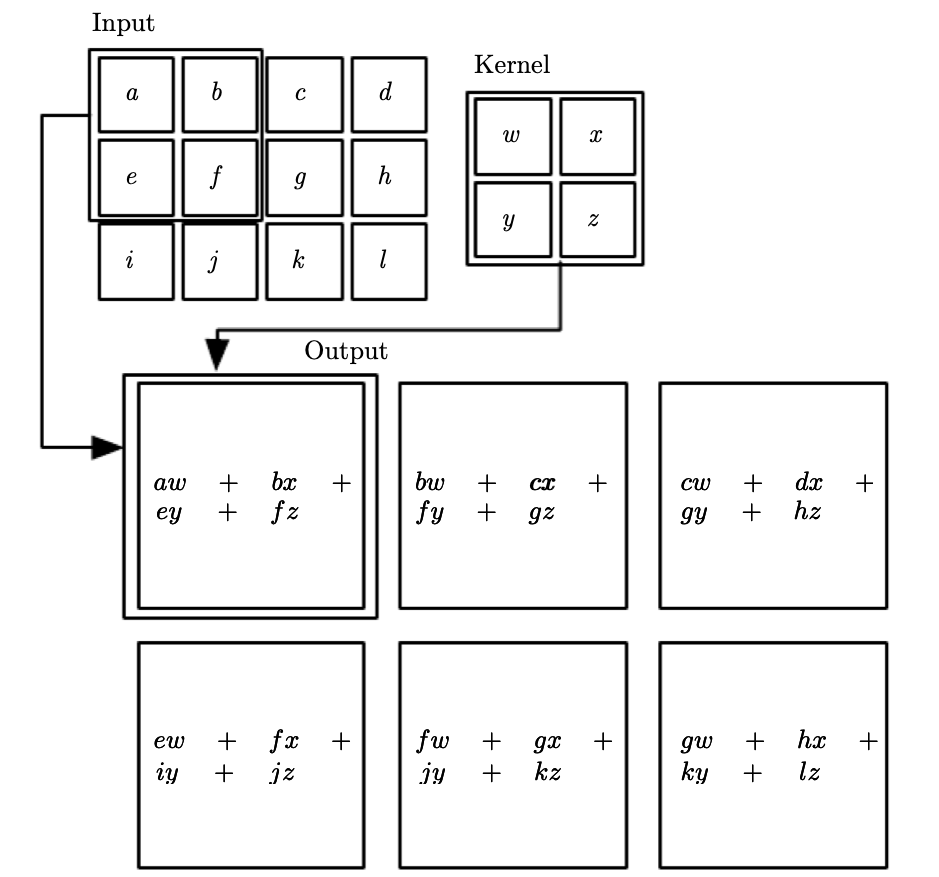
\includegraphics[width=0.6\textwidth]{capitulo2/figuras/an10.png}
	\caption[Convolución valida 2-D sin kernel volteado]{Convolución valida 2-D sin kernel volteado
		\\\textit{Fuente: Extraído de} \protect\cite[p. 334]{goodfellow2016deep}}
	\label{fig:an10}
\end{figure}

Comúnmente, la operación de convolución se representa con un asterisco. ver ecuación \ref{eq:e16}.

\begin{equation} \label{eq:e16} 
	s(i,j)=(I\ast K)
\end{equation}

Por ejemplo, en el caso de que se use un vector bidimensional I como entrada y un núcleo bidimensional K, la operación de convolución sería equivalente a la ecuación \ref{eq:e17} :

\begin{equation} \label{eq:e17} 
	S(i,j)=(I\ast K)(i,j)=\sum_{m}^{}\sum_{n}^{}I(m,n)K(i-m,j-n)
\end{equation}

Si se quiere invertir el núcleo, en el dado caso que se pueda aprovechar la conmutatividad de la operación de convolución, su representación se encuentra en la ecuación \ref{eq:e18}. Donde la  diferencia principal de la ecuación \ref{eq:e17} radica en el orden de los índices de desplazamiento de las variables de la convolución. Ya que a medida que m y n aumentan, los índices de la entrada aumentan, mientras que los de los índices del núcleo disminuyen.

\begin{equation} \label{eq:e18} 
	S(i,j)=(K\ast I)(i,j)=\sum_{m}^{}\sum_{n}^{}I(i-m,j-n)K(m,n)
\end{equation}

Muchas bibliotecas de redes neuronales implementan una función relacionada llamada correlación cruzada como muestra la ecuación \ref{eq:e19}, qué es lo mismo que la convolución pero sin invertir el núcleo.
\begin{equation} \label{eq:e19} 
	(I\ast K)(i,j)=\sum_{m}^{}\sum_{n}^{}I(i+m,j+n)K(m,n)
\end{equation}


La operación de convolución es un paso más para generar el necesario mapa de características, en el caso de que la entrada sea texto se  aplica el filtro w a una ventana de palabras  para crear una nueva característica. Por ejemplo, una característica $c_i$ se genera mediante la mediante la ecuación :

\begin{equation} \label{eq:e20} 
	c_i = f(\mathbf{w}\cdot \mathbf{x}_{i:i+h-1} + b)
\end{equation}
 

	
En la ecuación \ref{eq:e20} $b$ representa el término de sesgo, y $f$ es una función no lineal. El filtro en este caso representado por $w$ se emplea en cada ventana posible de palabras $x_i:i+h-1$ en la oración para generar un mapa de características $c=[c_1,c_2,\ldots,c_{n-h+1}]$. Es decir que, una vez que la entrada pasa por la capa de convolución y se le suma el sesgo, entonces se le aplicará una funcion de activacion para generar salidas no lineales a la entrada para finalmente aplicar la operación de pooling que se detallara más adelante.

 \textbf{Padding}
 
 El padding (relleno) se refiere a agregar valores adicionales alrededor de los bordes de la entrada antes de aplicar el filtro de convolución. Este proceso se utiliza para controlar el tamaño de la salida después de la operación de convolución.
Cuando se aplica un filtro a una entrada en una CNN, el tamaño de la salida se reduce debido a que el filtro no puede aplicarse a los bordes de la entrada. El padding resuelve este problema agregando filas y columnas adicionales de ceros o valores específicos alrededor de la entrada. Estos valores adicionales actúan como un ``borde'' alrededor de la entrada y permiten que el filtro se aplique a las regiones de los bordes de manera más efectiva.

Hay tres tipos comunes de padding: 

\begin{itemize}

	\item Padding ``same'' agrega suficientes filas y columnas de ceros alrededor de la entrada para asegurar que la salida tenga el mismo tamaño que la entrada original después de la convolución. ``En este caso, la red puede contener tantas capas convolucionales como el hardware disponible pueda soportar, ya que la operación de convolución no modifica las posibilidades arquitectónicas disponibles para la siguiente capa.''\cite[p. 350]{goodfellow2016deep}. Sin embargo, los elementos de la entrada cerca del borde influyen en menos elementos de salida que los elementos de la entrada cerca del centro, esto puede hacer que los elementos del borde estén algo subrepresentados en el modelo.
	
	\item Padding ``valid'' no agrega ningún relleno y permite que el filtro se aplique solo a las regiones donde el filtro y la entrada se superponen completamente, lo que produce una salida más pequeña que la entrada. ``Si la imagen de entrada tiene un ancho $m$ y el núcleo tiene un ancho $k$, la salida será de ancho $m - k + 1$. La tasa de esta contracción puede ser dramática si los núcleos utilizados son grandes.'' \cite[p. 350]{goodfellow2016deep}.
	
	\item Padding ``full'' se agregan ceros de tal manera que cada elemento en el borde sea visitado k veces, en cada dirección por el núcleo de convolución. Esto se traduce en una  salida que tiene un ancho mayor  que la entrada original, generalmente $m + k - 1$. En esta configuración, los elementos en los bordes de la  de salida están influenciados por menos elementos de la  entrada que los elementos más cercanos al centro. Esta disparidad puede dificultar que un único núcleo funcione de manera óptima en todas las posiciones del mapa de características.
	
\end{itemize}

El uso de padding en una CNN es crucial para controlar el tamaño de la salida y preservar la información en los bordes de la entrada durante la convolución. Esto es especialmente importante cuando se desean mantener detalles espaciales importantes en la imagen o secuencia de entrada. ``Por lo general, la cantidad óptima de relleno de ceros (en términos de precisión de clasificación del conjunto de pruebas) se encuentra en algún lugar entre la convolución ``válid'' y  ``same''.''\cite[p.350]{goodfellow2016deep}.

\textbf{Stride}

El stride (paso) se refiere a la cantidad de desplazamiento que se aplica al filtro convolucional a medida que se mueve a lo largo de la entrada. Un stride mayor significa que el filtro se mueve en incrementos más grandes, lo que resulta en una reducción del tamaño espacial de la salida. Por otro lado, un stride menor permite un solapamiento más grande entre las operaciones de convolución sucesivas y produce una salida con mayor tamaño espacial.
El ajuste del stride en una CNN puede influir en la dimensionalidad de la salida de cada capa convolucional, lo que a su vez puede afectar el número de parámetros y la información espacial conservada en la red. El stride se elige considerando la complejidad del problema, la dimensionalidad de la entrada y las características que se desean extraer de los datos.


	
\subsection{Capa de agrupación (pooling)}
La capa de agrupación (Pooling Layer) es una etapa crucial que sigue a las capas convolucionales. Su objetivo principal es reducir la dimensionalidad espacial de la representación convolucional, manteniendo las características más importantes.

Hay dos tipos comunes de funciones de agrupación:

\begin{itemize}
	
	\item Max Pooling: Esta función selecciona el valor máximo de una región dentro de la representación convolucional. Ayuda a resaltar las características más relevantes mientras reduce la cantidad de datos y, por ende, el procesamiento necesario.
	
	\item Average Pooling: En esta función, se toma el promedio de los valores dentro de la región seleccionada en lugar de escoger el máximo. Aunque es menos común que Max Pooling, se utiliza para reducir la dimensionalidad manteniendo información general.
	
\end{itemize}

Ambos tipos de funciones de agrupación ayudan a lograr invarianza espacial, lo que significa que la red es capaz de identificar patrones relevantes independientemente de su posición exacta en la imagen o secuencia de entrada.


\subsection{Capa totalmente conectada (fully connected layer)}
El uso de capas totalmente conectadas en una CNN no es obligatorio, depende en gran medida del problema específico y de la arquitectura de la red. Son útiles cuando se necesita combinar y procesar de manera integral las características extraídas por las capas convolucionales y de agrupación para realizar la tarea específica, como la clasificación de imágenes o el procesamiento de texto. Así que después de la extracción de características, se pueden agregar capas densamente conectadas para la clasificación final.

\textbf{Flatten}

La operación de ``flatten'' (aplanado) se refiere a una operación utilizada en redes neuronales para convertir una matriz multidimensional o un tensor en un vector unidimensional. Esta operación toma todas las dimensiones de la entrada y las combina en una única dimensión, conservando todos los elementos pero organizándolos en una única fila.
Después de pasar por varias capas convolucionales y de agrupación (pooling) en la CNN, por ejemplo, se obtiene una salida en forma de tensor tridimensional o multidimensional. Esta salida generalmente se transforma a una forma plana o un vector unidimensional antes de ser alimentada a capas densamente conectadas o totalmente conectadas, ya que las capas densas requieren una entrada en forma de vector unidimensional, para realizar la clasificación final o tareas similares.


\subsection{Métricas de evaluación}
A continuación se presentan algunas métricas de evaluación utilizadas para modelos de aprendizaje supervisado:

\begin{itemize}

\item Precisión(Precision): Esta métrica se enfoca en las predicciones positivas y mide cuántas de estas predicciones son realmente correctas. Ver ecuación \ref{eq:e25}.

Es importante distinguir esta métrica de la precisión global o exactitud, que evalúa todas las predicciones correctas (tanto positivas como negativas) en relación con el total de predicciones, misma que se ha estado utilizando hasta ahora en la evaluación de los modelos, ver ecuación \ref{eq:e26}.


\begin{equation} \label{eq:e25} 
	\text{Precisión} = \frac{\text{Verdaderos positivos}}{\text{Verdaderos positivos} + \text{Falsos positivos}}
\end{equation}

\begin{equation} \label{eq:e26} 
	\text{Accuracy} = \frac{\text{Número de predicciones correctas}}{\text{Número total de predicciones} }
\end{equation}

\item Sensibilidad (Recall): Es una métrica que mide la capacidad de un modelo para identificar correctamente todas las instancias de una clase positiva, ver ecuación \ref{eq:e27}.

\begin{equation} \label{eq:e27} 
	\text{Sensibilidad} = \frac{\text{Verdaderos positivos}}{\text{Falsos negativos} + \text{Verdaderos positivos} }
\end{equation}

La sensibilidad alta indica que el modelo es efectivo en detectar la mayoría de los casos positivos, aunque no mide los falsos positivos.

\item Puntaje F1 (F1 Score): Es una métrica que combina la precisión y la sensibilidad en una sola medida, utilizando la media armónica de ambas. Proporciona un equilibrio entre precisión y sensibilidad, ver ecuación \ref{eq:e28}.

\begin{equation} \label{eq:e28}
	\text{F1 Score} = 2 \cdot \frac{\text{Precisión}\cdot\text{Sensibilidad}}{\text{Precisión} + \text{Sensibilidad} }
\end{equation}

\item Matriz de Confusión: Es una representación visual que ayuda a comprender el rendimiento de un algoritmo de clasificación al comparar sus predicciones con los valores verdaderos. En problemas con más de dos clases, la matriz se expande a una matriz NxN, donde N es el número de clases. Los elementos en la diagonal principal indican las predicciones correctas para cada clase, mientras que los elementos fuera de la diagonal principal muestran los errores de clasificación, es decir, cuántas instancias de una clase fueron incorrectamente clasificadas como otra clase.

\end{itemize}

%\section{DIMENSIONALIDAD}
%Por defininir


\chapter{PROCESAMIENTO DEL LENGUAJE NATURAL Y CONJUNTO DE DATOS}\label{chp-controlIoT}
El Procesamiento del Lenguaje Natural (PLN) constituye un campo multidisciplinario que se centra en la interacción entre las computadoras y el lenguaje humano. Su objetivo principal es ayudar a las máquinas a comprender, interpretar y generar lenguaje natural de manera similar a la capacidad humana. En este capítulo, se proporciona una visión detallada que abarca desde los fundamentos teóricos hasta las técnicas modernas y las aplicaciones prácticas del PLN, lo que permite comprender tanto el estado actual como el potencial de este campo. Además, dada la escasez de conjuntos de datos que contienen lenguaje ofensivo en español, particularmente aquellos enfocados en el español de Bolivia, se detalla la creación de un conjunto de datos específico. Este conjunto de datos resultara sumamente útil para ser empleado por los modelos de aprendizaje automático propuestos en este contexto.

\section{DEFINICIÓN}
El Procesamiento del Lenguaje Natural (PLN) emerge de la combinación entre la inteligencia artificial y la lingüística. A diferencia de las diversas tareas que pueden tratar el aprendizaje automático o el aprendizaje profundo, el pnl se enfoca en tareas relacionadas con cualquier lenguaje o idioma, que los seres humanos utilicen para comunicarse de manera cotidiana, ya sea oral o escrita, este tipo de lenguaje es inherente a las culturas y evoluciona orgánicamente a lo largo del tiempo.

Vajjala define el PLN como ``un área de la informática que se enfoca en métodos para analizar, modelar y comprender el lenguaje humano. Prácticamente toda aplicación inteligente que implica el lenguaje humano tiene raíces en el PLN'' \cite[p. 4]{vajjala2020practical}.
 
El procesamiento del lenguaje natural, el aprendizaje profundo y el aprendizaje automático son subcampos de la Inteligencia Artificial que, de hecho, se superponen  entre ellos, ver Figura \ref{fig:nlp1}.Ya que estas disciplinas colaboran entre sí e incluso sirven como base la una a la otra, como ocurre con el aprendizaje automático y el aprendizaje profundo, e igualmente  muchos modelos de lenguaje hacen uso tanto del aprendizaje profundo como de técnicas tradicionales del aprendizaje automático. Sin embargo esto no evita que cada una de estas disciplinas tenga su área específica de estudio. Como el PLN que, se concentra en el análisis y comprensión del lenguaje humano, explorando diversas técnicas para estos propósitos.

\begin{figure}
	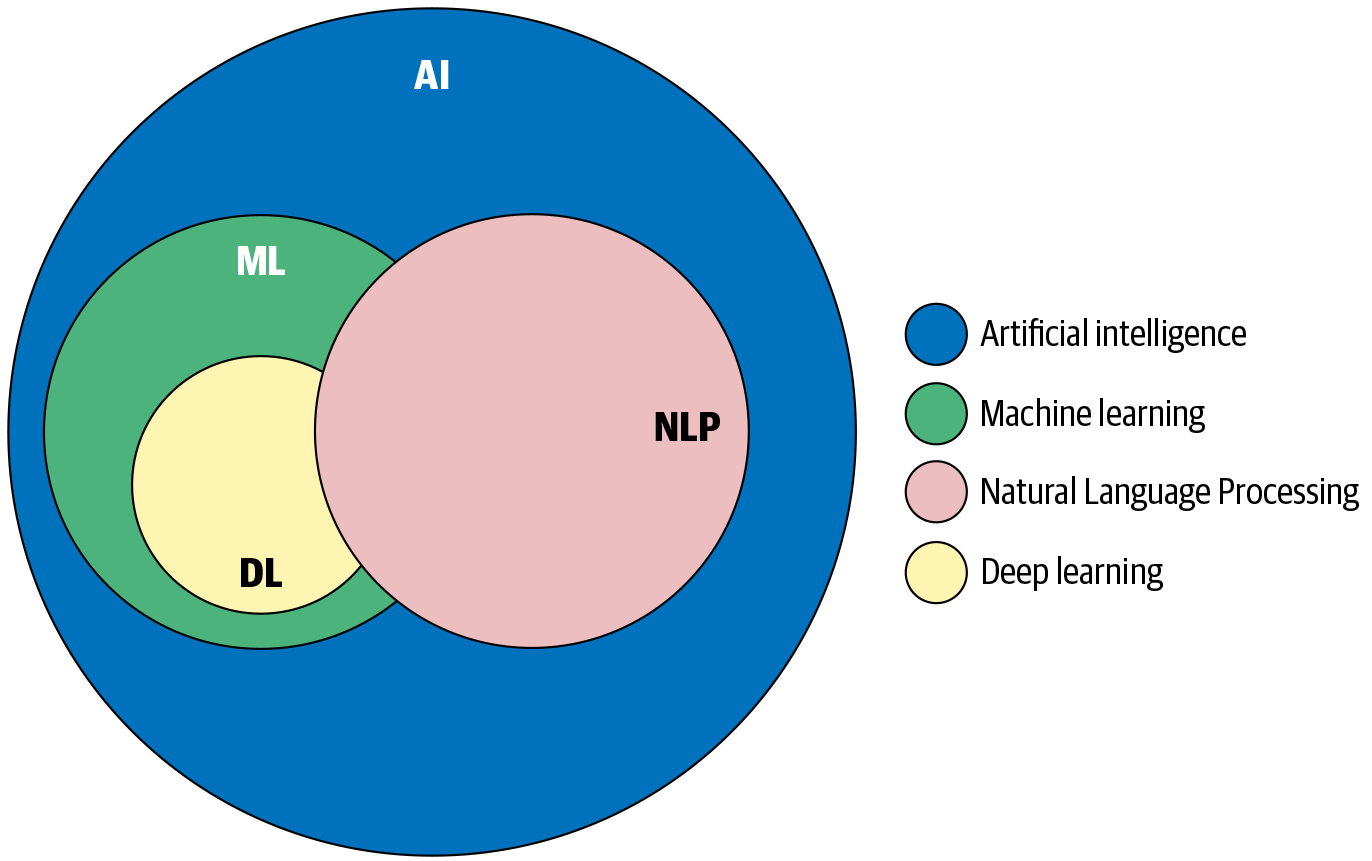
\includegraphics[width=0.65\textwidth]{capitulo3/figuras/nlp1.png}
	\caption{Como NLP, ML, y DL se relacionan}
	\floatfoot{Fuente: Practical natural language processing: A comprehensive guide to building real-world NLP systems \cite[p. 15]{vajjala2020practical} } 
	\label{fig:nlp1}
\end{figure}

\section{BREVE HISTORIA DEL PLN}
El Procesamiento del Lenguaje Natural (PLN) ha evolucionado desde los años 50, cuando Alan Turing planteó la posibilidad de evaluar la inteligencia de una máquina a través de conversaciones humanas en un artículo publicado en 1950 llamado ``Computing Machinery and Intelligence'' (Máquinas de computación e inteligencia) \cite{turing2009computing}. En la década de los 60, se desarrollaron los primeros programas de traducción automática y análisis gramatical. Uno de los primeros sistemas de PLN fue el ``ELIZA'', creado por Joseph Weizenbaum en 1966, que simulaba una conversación terapéutica \cite{weizenbaum1966eliza}.

En los años 70, la influencia de la Gramática Generativa Transformacional de Noam Chomsky fue significativa en el ámbito del Procesamiento del Lenguaje Natural (PLN). Esta teoría lingüística propuesta por Chomsky en las décadas anteriores buscaba establecer reglas abstractas y universales para explicar cómo se generan y estructuran las oraciones en cualquier lengua \cite{chomsky1970remarks}.

En ese período, los modelos de PLN estaban fuertemente influenciados por esta perspectiva basada en reglas. Se intentaba aplicar las ideas de la gramática generativa a la comprensión del lenguaje natural mediante la creación de sistemas computacionales que imitaran, en cierta medida, las reglas y principios gramaticales identificados por Chomsky. Estos sistemas se centraban en la construcción de reglas para analizar y procesar el lenguaje.

En los 80 hubo un cambio en el enfoque utilizado en los sistemas de PLN. Se adoptaron sistemas basados en el conocimiento y la codificación manual de reglas. En lugar de depender únicamente de los principios gramaticales generales, se codificaba manualmente reglas y patrones lingüísticos que se consideraban relevantes para las tareas específicas

El avance hacia los 90 trajo consigo la introducción de métodos estadísticos y basados en el aprendizaje automático en el PLN, junto con el crecimiento de la web que impulsó la necesidad de herramientas de búsqueda y análisis de texto a gran escala.

Desde el año 2000 en adelante, el PLN se ha expandido enormemente y se ha convertido en un campo multidisciplinario que incorpora el aprendizaje profundo, modelos basados en la estadística, el procesamiento de grandes volúmenes de datos (big data) y la aplicación de técnicas avanzadas en áreas como la comprensión del lenguaje, la traducción automática y los chatbots.

Esta rápida evolución continúa en la actualidad, con el PLN jugando un papel crucial en numerosas aplicaciones, desde motores de búsqueda hasta asistentes virtuales y análisis de sentimientos en redes sociales.

\section{TAREAS DE PLN}
El Procesamiento del Lenguaje Natural  abarca una gran variedad de tareas que se han vuelto imprescindibles para las personas, las mismas que  nos muestran una increíble evolución en la aplicabilidad de esta disciplina . Algunas de las tareas más comunes en PLN son:

\begin{itemize}

	\item Clasificación de Texto: Esta es una de las tareas más populares, se encarga de asignar etiquetas o categorías a un texto dado. Ejemplos incluyen la detección de spam en correos electrónicos o la clasificación de noticias por tema.

	\item Extracción de Información: Implica identificar y extraer información específica de textos, como nombres de personas, ubicaciones, fechas, etc., desde artículos o documentos.

	\item Análisis de Sentimientos: Determina la actitud emocional detrás de un texto, ya sea positiva, negativa o neutral. Es útil para evaluar opiniones en redes sociales, reseñas de productos, etc.

	\item Generación de Lenguaje Natural: Crear texto coherente y significativo, como resúmenes automáticos, diálogos generativos, entre otros.

	\item Reconocimiento de Entidades Nombradas (NER): identificar y clasificar entidades importantes en un texto, como nombres de personas, lugares, organizaciones, etc.

	\item Traducción automática: Convertir texto de un idioma a otro, lo que implica comprender y generar texto en diferentes lenguajes. Por ejemplo, la herramienta más popular que realiza la tarea de traducir actualmente más 100 idiomas es Google Translate.
	
	\item Modelado de Lenguaje: Esta tarea se encarga de  predecir la probabilidad de una secuencia de palabras en un idioma determinado, lo que se usa en corrección gramatical, autocompletado de texto, entre otros. 

\end{itemize}

Estas tareas son solo una muestra de las aplicaciones del PLN, cada una de ellas tiene su nivel de dificultad y su conjunto específico de métodos de resolución.


\section{LA CANALIZACIÓN PLN}
En el desarrollo de soluciones en PLN, es habitual desglosar el problema en componentes más pequeños y manejables. Esto implica identificar los requisitos esenciales y dividir el problema en varios subproblemas, cada uno de los cuales se aborda de manera individual.

Este enfoque incluye un detallado procesamiento de texto en cada fase, el mismo es conocido como canalización del procesamiento de lenguaje natural y representa la serie de pasos necesarios para construir cualquier modelo de PLN. Estos pasos se encuentran omnipresentes en los proyectos de PLN, convirtiéndolos en un requisito en este campo, la visualización de estas etapas clave del proceso, su relación y orden se puede observar en la figura 2.1.

-------------------------------------------

figura 2.1

-----------------------------------------

A continuación se detalla específicamente todo este proceso paso por paso, para el tratamiento de texto y su uso en modelos de aprendizaje automático.


\subsection{Adquisición de datos}
La adquisición de datos en el Procesamiento del Lenguaje Natural (PLN) es un primer paso crucial en el desarrollo de cualquier sistema de procesamiento de texto.

Comprende la obtención de datos relevantes que se utilizarán para entrenar modelos, realizar pruebas y validar algoritmos en un contexto específico. Estos datos pueden provenir de diversas fuentes, como documentos escritos, transcripciones de audio, redes sociales, páginas web, entre otros.

Esta etapa implica la identificación de las fuentes de datos disponibles y la posterior obtención  de información en función de las necesidades del proyecto. La calidad, cantidad y diversidad de los datos adquiridos son factores cruciales para el rendimiento y la precisión de los modelos de PLN.  Las maneras de recolectar y generar información pueden ser las siguientes:

\begin{itemize}

	\item Usar un conjunto de datos (dataset)  público.- En primer lugar, buscar conjuntos de datos públicos que se puedan usar para la tarea que se quiere resolver, es una buena opción. Se pueden encontrar conjuntos de datos recopilados por algunas personas como los de Nicolas Iderhoff en su repositorio de github o mediante motores de búsqueda especializados como el de Google para datasets o kaggle. Sin embargo es muy importante tener en cuenta que a pesar de que se esté tratando con un conjunto de datos listo para usarse, es muy importante considerar el equilibrio, limpieza, utilidad y otras importantes características que debe contener el dataset.
	
	\item Raspado de datos (Scrape data).-  Una opción es la recolección de datos relevantes de fuentes en línea, como foros de discusión, plataformas de consumidores, redes sociales, seguido de la anotación humana. Si no se necesita obtener datos con detalles específicos el raspado de datos es una buena pero costosa opción debido al tiempo que debe invertirse para raspar miles y miles de datos.

\end{itemize}


\textbf{Aumento de datos}

El PNL ofrece una variedad de técnicas que permiten ampliar un conjunto de datos reducido mediante métodos conocidos como aumento de datos. Estas estrategias buscan aprovechar las propiedades del lenguaje para generar texto adicional que mantenga similitudes con los datos originales. A continuación, se detallara algunas de estas técnicas:

\begin{itemize}

	\item Reemplazo de sinónimos: Consiste en seleccionar aleatoriamente ``k'' palabras en una oración que no sean palabras vacías(a, el, ella, un) y reemplazarlas por sus sinónimos.
	
	\item Traducción inversa: Se puede tomar una oración (S1) en español y traducirla a otro idioma, por ejemplo, inglés.  La oración correspondiente en inglés sería (S2). Luego, se traducirá nuevamente S2 al español, obteniendo una nueva oración (S3). Para generar y asegurar un poco más la variedad, también puede ser conveniente usar distintas herramientas de traducción.
	
	\item Reemplazo de palabras basado en TF-IDF: La traducción inversa podría perder palabras cruciales, es por eso que se utilizan los pesos TF-IDF para determinar qué palabras son más cruciales en una oración. Aquellas palabras con pesos TF-IDF más altos tienen una contribución más significativa al significado de la oración. Por lo tanto, al generar datos adicionales, se reemplazan las palabras menos importantes con sus sinónimos o palabras similares de acuerdo con sus pesos TF-IDF. Esto permite mantener la esencia semántica de la oración mientras se generan datos adicionales.
	
	\item Inversión de bigramas: Se divide la oración en bigramas y se selecciona uno al azar para invertir. Por ejemplo, en ``Voy al supermercado'', se toma el bigrama ``al supermercado'' y se invierte: ``voy''.
	
	\item Reemplazo de entidades: Consiste en cambiar entidades como nombres de personas, lugares, organizaciones, etc., por otras en la misma categoría. Por ejemplo, en ``Vivo en Bolivia'', reemplazar ``Bolivia'' por ``Perú''.
	
	\item Agregar ruido a los datos: En muchas plataformas los datos entrantes contienen errores ortográficos, como por ejemplo cualquier red social (Twitter, Instagram, Facebook). Para que el modelo pueda lidiar con este problema es importante agregar un poco de ruido a los datos, para que así se permita entrenar un modelo más robusto. Por ejemplo, reemplazar una palabra en una oración por otra similar en ortografía. Otro tipo de ruido proviene de los errores de teclado en dispositivos móviles, donde se simula un error de teclado QWERTY reemplazando algunos caracteres por sus vecinos en el teclado.

	\item Técnicas Avanzadas: En la búsqueda de expandir conjuntos de datos textuales, existen técnicas y sistemas avanzados notables como Snorkel, que sobresale al permitir la generación automatizada de datos de entrenamiento sin requerir etiquetado manual, empleando heurísticas y transformaciones sobre los datos existentes para crear muestras sintéticas de alta calidad. Por otro lado, herramientas como Easy Data Augmentation (EDA) y NLPAug igualmente ofrecen un abanico de técnicas para la ampliación de datos y creación de datos sintéticos.
	
	\item Etiquetado de datos: Una ayuda para el etiquetado de miles de datos puede ser el aprendizaje activo. Es un enfoque específico dentro del aprendizaje automático que implica la interacción entre el algoritmo de aprendizaje y un experto humano para etiquetar datos. Se utiliza en situaciones donde hay un gran conjunto de datos sin etiquetar, pero el proceso de etiquetado manual es costoso o consume mucho tiempo. La idea clave radica en determinar qué instancias específicas de datos deberían ser solicitadas para ser etiquetadas, con el objetivo de maximizar el aprendizaje del algoritmo y, al mismo tiempo, minimizar el costo y la cantidad de datos etiquetados requeridos. Es esencial identificar estratégicamente los puntos de datos que pueden proporcionar la mayor información para mejorar el rendimiento del modelo, optimizando así el proceso de etiquetado.

\end{itemize}


\subsection{Preprocesamiento de texto}
El preprocesamiento de texto es un paso fundamental que implica la transformación y limpieza de datos de texto para que sean más adecuados y efectivos para su análisis por algoritmos de aprendizaje automático. Aquí hay algunas técnicas comunes utilizadas en el preprocesamiento de texto en NLP:

\begin{itemize}

	\item Segmentación de oraciones: Dividir texto en oraciones individuales implica identificar los límites entre oraciones basándose en reglas gramaticales, puntuación (como puntos, signos de interrogación, etc.) y contextos lingüísticos. Pero si el texto que se quiere dividir no contiene puntos, comas o cualquier otro carácter que indique un límite se debe encontrar alguna otra manera de dividirlo ``Como regla simple, podemos segmentar oraciones dividiendo el texto en oraciones cuando aparecen puntos y signos de interrogación. Sin embargo, puede haber abreviaturas, formas de direcciones (Dr., Sr., etc.), o elipses (...) que pueden romper la simple regla. Afortunadamente, la mayoría de las bibliotecas de PNL vienen con algún tipo de división de oraciones y palabras implementada. Una biblioteca de uso común es Natural Language Tool Kit (NLTK)''. \cite[p.50]{vajjala2020practical}.

	\item Word tokenization: implica dividir un texto en unidades más pequeñas llamadas ``tokens''. Estos tokens suelen representar palabras individuales, aunque en algunos casos pueden ser partes más pequeñas de palabras, números, signos de puntuación, etc. La tokenización se realiza típicamente antes de aplicar cualquier análisis o modelado de texto.

	\item Lematización y derivación: La derivación consiste en reducir las palabras a una forma más simple, para reducir la variabilidad y normalizar el texto. Ver parte derecha de la Figura \ref{fig:nlp2}.``La derivación se refiere al proceso de eliminar sufijos y reducir una palabra a alguna forma básica por ejemplo: ``auto'' y ``autos'' se reducen a ``auto'' Esto se logra aplicando un conjunto fijo de reglas, la derivación se usa en la clasificación de textos para reducir el espacio de funciones para entrenar modelos de aprendizaje automático.''\cite[p. 53]{vajjala2020practical}.


Lematizar es un proceso que consiste en reducir las palabras a sus formas base. Por ejemplo ``eres'' se lematiza como ``ser''. Aunque se parece a la derivación la principal diferencia radica en el proceso mucho más exhaustivo que implica no solamente eliminar sufijos o reducir la palabra.Ver Figura \ref{fig:nlp2} ``La lematización es el proceso de mapear todas las diferentes formas de una palabra a su palabra base, o lema. La lematización requiere más conocimiento lingüístico, y modelar y desarrollar lematizadores eficientes sigue siendo un problema abierto en la investigación de PNL incluso ahora.'' \cite[p. 53]{vajjala2020practical}.

\begin{figure}[h!]
	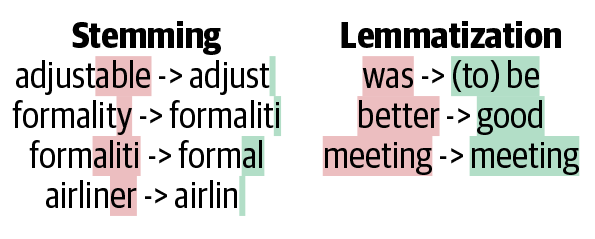
\includegraphics[width=0.65\textwidth]{capitulo3/figuras/nlp2.png}
	\caption{Diferencias entre la derivación y lematizacion
		\\\textit{Fuente: Extraído de} \protect\cite[p. 54]{vajjala2020practical}}
	\label{fig:nlp2}
\end{figure}
	
	\item Eliminar caracteres no alfabéticos: Eliminar signos de puntuación, números, símbolos, direcciones web y otros caracteres no alfabéticos simplifica el texto para un análisis y procesamiento más sencillo. La eliminación de estos caracteres innecesarios reduce el ruido en el análisis, mejorando la calidad y precisión de los modelos. Para esta tarea específica, el uso de expresiones regulares en funciones es altamente recomendado, ya que el tratamiento de cada conjunto de datos es diferente, debido a que cada uno tiene sus propias particularidades.
	
	\item Minúsculas: Transformar todo el texto en minúsculas es importante para unificar el tratamiento de palabras. Esta normalización del texto asegura una representación uniforme de las palabras bajo un mismo sistema de codificación, evitando que el modelo distinga entre palabras escritas con mayúsculas o minúsculas. Además, reduce la carga computacional al disminuir la cantidad de palabras distintas que el modelo necesita procesar, lo que mejora la eficiencia del análisis.

	\item Eliminar stopwords: Eliminar palabras comunes (stopwords) que no agregan valor al análisis, como ``el'', ``la'', ``y'', etc. Estas palabras son frecuentes en el lenguaje y aparecen en casi todos los textos. Al eliminarlas, se reduce la dimensionalidad del espacio de características y hace que el enfoque se centre en palabras clave y términos más significativos para el análisis.
	
	\item Corrección de errores ortográficos: Identificar y corregir errores ortográficos puede mejorar la precisión del análisis. Su efectividad puede variar dependiendo del contexto y del propósito del análisis. En entornos donde la precisión en la escritura es esencial, como la traducción automática o el análisis de sentimientos, corregir los errores ortográficos puede ser beneficioso. En ciertos casos, especialmente en análisis de texto informal o en redes sociales, conservar los errores ortográficos puede ser importante para capturar el tono o el estilo del texto original.
	
	\item Tratamiento de emojis: Los emojis son representaciones visuales cuya presencia puede ser crucial para comprender el tono, la intención o las emociones expresadas en un texto. En algunos casos, es útil eliminar los emojis del texto si no aportan información relevante para la tarea de procesamiento o análisis. En otros casos los emojis pueden mapearse a palabras o frases que describan su significado o intención. Por ejemplo, un emoji sonriente podría ser mapeado a la palabra ``feliz'' o ``contento'', mientras que un emoji de tristeza podría mapearse a ``triste'' o ``decepcionado''. 
Si no se decide hacer ninguno de los pasos anteriores y se considera mantenerlos en su estado original es importante convertir estos caracteres especiales a una representación más simple para su tratamiento.``Para analizar dichos símbolos no textuales y caracteres especiales, utilizamos la normalización Unicode. Esto significa que el texto que vemos debe convertirse en alguna forma de representación binaria para almacenarlo en una computadora. Este proceso se conoce como codificación de texto. Ignorar los problemas de codificación puede provocar errores de procesamiento en el futuro.''\cite[p. 45]{vajjala2020practical}.

\end{itemize}

El preprocesamiento de texto es esencial para preparar los datos de texto para su análisis, ayudando a eliminar ruido, reducir la dimensionalidad y mejorar la calidad de los datos, antes de aplicarlo a modelos de aprendizaje automático en tareas de NLP. También es importante mencionar que cada uno de los pasos de tratamiento de texto ya detallados no son obligatorios en su aplicación, que aplicar, en qué momento u orden depende solamente de lo que le convenga a la tarea que se quiere realizar 
	
	
	

\subsection{Representación de texto}
Si bien representar características es común en todo proyecto de ML, hacerlo con texto suele ser más complejo que con otros tipos de datos. Consideremos ejemplos como imágenes: almacenamos imágenes como matrices de píxeles, cada uno representando la intensidad de un píxel en la imagen. Con videos, cada cuadro se convierte en una matriz. En cuanto al habla, registramos la amplitud de una onda sonora en intervalos de tiempo fijos. Sin embargo, representar matemáticamente texto después de haberlo dividido en alguna unidad léxica para luego deducir el significado de cada unidad, comprender la estructura gramatical, entender el contexto en el que aparece y finalmente gracias a estos datos discernir la semántica, no es tan fácil. Esta sección  se sumerge en múltiples esquemas para abordar esta complejidad, desde métodos simples hasta las últimas técnicas para representar texto, un desafío que ha sido un foco activo de investigación en las últimas décadas.

Los enfoques tomados para generar todo tipo de representaciones de texto que se detallaran a continuación, pueden ser: 

\begin{itemize}

	\item Similitud Distribucional : El significado de una palabra se extrae del contexto en el que aparece, no sólo del significado literal.

	\item Hipótesis Distribucional: Plantea que palabras en contextos similares tienen significados similares. La similitud entre palabras se basa en sus contextos de aparición.
	
	\item Representación Distribucional: Se basa en esquemas que utilizan vectores de alta dimensión para representar palabras, basados en una matriz de co-ocurrencia, misma que captura la co-ocurrencia de palabras y contextos.
	
	\item Representación Distribuida: Una versión más compacta y densa en vectores que la representación distribucional, para superar la ineficiencia computacional de los vectores altamente dimensionales.

	\item Incrustación: Es un mapeo entre el espacio vectorial de la representación distributiva y la representación distribuida para un conjunto de palabras.
	
	\item Semántica Vectorial: Métodos de PLN que buscan aprender representaciones de palabras basadas en propiedades distribucionales en grandes corpus.
\end{itemize}

En el campo del PNL, transformar texto en una forma numérica se llama representación de texto. A continuación se explorarán los distintos métodos para convertir texto en vectores numéricos, todos los que se encuentran clasificados como modelos espaciales vectoriales como one-hot, bag of words, bag of n-grams y TF-IDF  caen dentro del concepto de representación distribucional.

\begin{itemize}
\item Modelos espaciales vectoriales


Los modelos vectoriales espaciales son técnicas que representan las palabras como vectores en un espacio dimensional. Estos modelos tienen como objetivo capturar la semántica de las palabras al asignarles vectores en un espacio matemático, donde la proximidad entre los vectores refleja la similitud semántica entre las palabras. Un modelo de espacio vectorial  es un modelo algebraico simple, en su representación simple son vectores identificadores como un índice de números en un vocabulario de algún documento, párrafo o libro de texto. El modelo más común para medir esta similitud, es la similitud del coseno, ver ecuacion \ref{eq:e21}. Por ejemplo las frases: ``El cielo es azul'' y ``El sol es amarillo'', se pueden representar cada una como un vector numérico. Para calcular la similitud entre estos vectores, se puede utilizar  el coseno del ángulo entre ellos. Si estos vectores se alinean perfectamente, el coseno del ángulo es 1, lo que indica una similitud máxima. Si están en direcciones opuestas, el coseno es -1, lo que significa una similitud mínima.
\begin{equation} \label{eq:e21} 
	similarity = cos(\theta) = \frac{\mathbf{A} \cdot \mathbf{B}}{\left \|  \mathbf{A} \right \|_2\cdot \left \|  \mathbf{B} \right \|_2}=\frac{\displaystyle\sum_{i=1}^{n}A_iB_i}{\sqrt{\displaystyle\sum_{i=1}^{n}A_i^2}\sqrt{\displaystyle\sum_{i=1}^{n}B_i^2}}
\end{equation}


$A = $  Algun vector.\\
$B = $  Algun vector.\\
$\mathbf{A} \cdot \mathbf{B} =$ Es el producto punto entre los vectores $A$ y $B$.\\
$\left \|  \mathbf{A} \right \|_2\cdot \left \|  \mathbf{B} \right \|_2 = $ Indica la norma euclidiana o la norma $L_2$. \\
$L_2$  de un vector = Se calcula sumando el cuadrado de cada componente del vector y luego tomando la raíz cuadrada del resultado. Que es equivalente a: 
$\left \|  \mathbf{A} \right \|_2 = \sqrt{A_1^2 + A_2^2 + \cdots + A_n^2} $.\\


La calidad de los vectores depende de cómo capturan las propiedades lingüísticas del texto. Diferentes enfoques, como el conteo de palabras o modelos de lenguaje pre-entrenados (word embeddings), producen representaciones de texto en forma de vectores con diferentes niveles de fidelidad y utilidad.

\begin{itemize}

	\item ONE HOT ENCODING: En One-Hot Encoding, cada palabra se representa mediante un vector binario donde todas las posiciones son cero excepto una, que corresponde al índice de la palabra en un vocabulario. Si hay un total de N palabras en el vocabulario, cada palabra se representa como un vector de longitud N con un único ``1'' en la posición que indica su índice en el vocabulario y ``0'' en todas las demás posiciones. Por ejemplo, si se tiene un vocabulario con las palabras: ``perro'', ``gato'', ``pájaro'' y ``muerde'', la representación One-Hot de cada una sería:
\begin{Center}
	perro → [1, 0, 0,0]\\
	gato → [0, 1, 0,0]\\
	pájaro → [0, 0, 1,0]\\
	muerde → [0, 0, 0, 1]\\
	
\end{Center}

Donde:

La oración ``perro muerde gato'' sería representada como: [   [1, 0 ,0 , 0]   [0, 0, 0, 1]   [0, 1, 0, 0]  ]


Este tipo de representación textual  es intuitiva y fácil de implementar pero, presenta limitaciones significativas. La relación directa entre el tamaño del vector one-hot y el tamaño del vocabulario provoca representaciones dispersas donde la mayoría de las entradas son ceros, lo que resulta en ineficiencia computacional y riesgo de sobreajuste. Además, esta representación no ofrece una longitud fija para el texto y trata las palabras como entidades aisladas, careciendo de la capacidad para capturar relaciones semánticas entre ellas. El desafío de manejar palabras fuera del vocabulario (Out Of Vocabulary), no se puede abordar directamente con esta representación, se requiere la expansión y reentrenamiento del modelo para incluir nuevas palabras.

	\item BAG OF WORDS: El modelo Bag of Words (BoW) es una técnica básica  para representar texto numéricamente. Primero  se construye un vocabulario a partir del corpus de documentos. El vocabulario se compone de todas las palabras únicas presentes en el corpus, y cada palabra se la enumera de manera única. Luego, se representa cada documento como un vector numérico. Para ello, se cuenta la frecuencia de cada palabra del vocabulario en cada documento. Por ejemplo: 
Dada las oraciones: \textit{``El gato está en la casa gato''} y \textit{``El perro está afuera''}

Se construye el diccionario: {El=1, gato=2, está=3, en=4, la=5, casa=6, perro=7, afuera=8}. Los IDs serán enteros únicos entre $\left | \text{V} \right |$, Donde $\left | \text{V} \right |$ representa el tamaño del vocabulario.

Se realiza la representación BoW:
\begin{center}[h!]
	\begin{tabular}{c c c c c c c c c c}
		& El & gato & está & en & la & casa & perro & afuera &  \\
		Frase 1: & 1 & 2 & 1 & 1 & 1 & 1 & 0 & 0 & ←Conteo frase 1\\
		Frase 2: & 1 & 0 & 1 & 0 & 0 & 0 & 1 & 1 & ←Conteo frase 2\\
		
	\end{tabular}
\end{center}


El enfoque de BoW trata el texto como una colección de palabras sin considerar el orden ni el contexto en el que aparecen. Supone que el contenido de un texto asociado a una categoría específica en un conjunto de datos está representado por un conjunto único de palabras. Si dos fragmentos de texto comparten la mayoría de sus palabras, se asume que pertenecen a la misma categoría o grupo, por esta razón se puede inferir la categoría o clase a la que ese texto puede pertenecer. Es importante resaltar que el enfoque BoW simplifica el texto a su esencia más básica: las palabras y su frecuencia, sin tomar en cuenta su secuencia o estructura gramatical.

	\item BAG OF N-GRAMS.- Es una técnica utilizada que extiende el concepto de Bag of Words (BoW) al considerar no solo palabras individuales, sino también secuencias contiguas de palabras llamadas n-gramas.``Capta cierta información de contexto y orden de palabras. Por tanto, el espacio vectorial resultante es capaz de capturar alguna similitud semántica. Los documentos que tienen los mismos n-gramas tendrán sus vectores más cerca entre sí en el espacio euclidiano en comparación con documentos con n-gramas completamente diferentes.''\cite[p. 90]{vajjala2020practical}. Un n-grama es una secuencia continua de ``n'' elementos, que pueden ser caracteres, palabras o algún tipo de token, a medida que n aumente, la dimensionalidad aumentará igual rápidamente. Por ejemplo:

Dadas las oraciones: ``El gato está durmiendo'' y ``El perro está comiendo''

Una representación bigrama de palabras es equivalente a:
[ ``El gato'', ``gato esta'', ``está durmiendo'', ``El perro'', ``perro esta'', ``está comiendo'' ]

La representación BoN constara de un vector de seis dimensiones para cada documento: ``El gato está durmiendo'' → [1,1,1,0,0,0], ``El perro está comiendo'' → [0,0,0,1,1,1 ].


Es importante recordar que al igual que Bag of Words, Bag of N-Grams (BoN) no ofrece una solución directa al problema de OOV (Out Of Vocabulary), es decir, no tiene un mecanismo incorporado para tratar con palabras que no estaban presentes durante el entrenamiento del modelo.


	\item TF-IDF.- A diferencia de las anteriores técnicas de representación de texto, Frecuencia de término-Frecuencia inversa de documentos (Term Frequency-Inverse Document Frequency) es una técnica que evalúa la importancia de una palabra en un documento dentro de un corpus o conjunto de documentos. Su formula general se divide en dos componentes que se explicaran detalladamente. Ver ecuación \ref{eq:e22}

\begin{equation} \label{eq:e22}
	\textrm{TF-IDF} = \textrm{TF} \times \textrm{IDF}
\end{equation}

TF (Frecuencia del término) mide la frecuencia con la que una palabra específica aparece en un documento en relación con el total de palabras en ese documento. Básicamente, es la cantidad de veces que una palabra aparece, dividida por el total de palabras en el documento como se muestra en la ecuacion \ref{eq:e23}. Si una palabra aparece muchas veces en un documento específico, y no aparece en los demás documentos, entonces se considera que la palabra es importante para ese documento específico.

\begin{equation} \label{eq:e23}
	\textrm{TF}(t,d)=\frac{(\textrm{Number of occurrences of term }t\textrm{ in document }d)}{(\textrm{Total number of terms in the document } d)}
\end{equation}

IDF (Frecuencia inversa de documentos) mide la importancia de una palabra a través de todo el conjunto de documentos. Esta métrica reduce el peso de palabras comunes que aparecen en muchos documentos y aumenta el peso de palabras raras que podrían ser más significativas para un documento específico. Es decir, si se considera que una palabra es importante para un documento, pero esta aparece constantemente en los demás documentos entonces disminuye su importancia. Se calcula tomando el logaritmo del inverso de la frecuencia de documentos que contienen el término, y se suma uno para evitar la división por cero si el término no está presente en el corpus.

\begin{equation} \label{eq:e24}
	\textrm{IDF}(t)=\frac{(\textrm{Total number of documents in the corpus})}{(\textrm{Number of documents with term } t \textrm{ in them})}
\end{equation}

Esta técnica de representación se aplica para cada palabra en cada documento y se  pueden usar los vectores obtenidos para calcular la similitud entre dos textos, usando alguna medida de similitud como la distancia euclidiana o la similitud del coseno.


\end{itemize}

\item Representaciones distribuidas

Las representaciones distribuidas de texto buscan capturar el significado de palabras, oraciones o frases considerando su proximidad textual, en un espacio vectorial. Estas representaciones, conocidas como embeddings, abordan los desafíos de dimensionalidad y contexto crucial durante el entrenamiento. Para lograrlo, emplean arquitecturas de redes neuronales que generan representaciones de baja dimensión y alta densidad para palabras y textos.

\begin{itemize}

	\item Word embeddings: Las incrustaciones de palabras (word embeddings) son representaciones vectoriales de palabras en un espacio dimensional, donde cada palabra se asigna a un vector denso. Estos vectores son diseñados de manera que palabras con significados similares están cercanas entre sí en este espacio vectorial, además sus representaciones vectoriales de texto tienen dimensiones bajas y densas en comparación con representaciones one-hot encoding, lo que permite una manipulación más eficiente. Los modelos  más populares pueden ser: Word2Vec, GloVe y FastText, uno de los mayores representantes de los modelos embeddings es Word2Vec, que en si mismo es un conjunto de modelos que fueron fundamentales en el campo del Procesamiento del Lenguaje Natural. Desarrollado por un equipo de investigadores de Google, liderado por Tomás Mikolov, en 2013, fue un avance crucial en la generación de representaciones vectoriales de palabras, basadas en modelos de redes neuronales, cuya idea central era capturar y representar la semántica de las palabras a través de sus contextos en un corpus de texto \cite{mikolov2013efficient}. 
	
	\item Hiperparametros de embeddings: Algunos hiperparámetros comunes al trabajar con embeddings en modelos como Word2vec, GloVe, fastText o incluso en modelos más avanzados incluyen:  La dimensión del embedding, la cual  determina la longitud de los vectores; la ventana de contexto, controla cuántas palabras vecinas se van a considerar y el tamaño del vocabulario, ya que algunos modelos de embeddings tienen un límite en el tamaño del vocabulario a usar. Ajustar estos y otros  hiperparámetros correctamente puede influir significativamente en la calidad y el rendimiento de los embeddings resultantes.``El ajuste de hiperparámetros juega un papel clave: cualquier método funcionará mal si se utilizan los hiperparámetros incorrectos'' \cite[p. 339]{eisenstein2018natural}.
	
	\item Word2Vec.- El modelo Word2Vec se destaca por su capacidad para generar incrustaciones vectoriales significativas y densas para palabras, lo que permite representar el significado semántico de las palabras en un espacio vectorial de dimensiones bajas (vectores de dimensiones 50-500 en vez de varios miles). Su eficiencia para la representación de palabras fue tal, que se observaron habilidades para resolver analogías y capturar relaciones de significado entre palabras como:  
	\begin{Center}
			$Rey - Hombre + Mujer \approx  Reina$.
	\end{Center}

	
Word2vec es un conjunto redes neuronales poco profundas que utilizan la similitud distributiva e hipótesis distributiva para aprender  el significado de las palabras ``El modelo Word2vec perfecciona los valores en $v_w$ al predecir $v_{w'}$, dados los vectores para las demás palabras en el contexto C.'' \cite[p. 95]{vajjala2020practical} .

Word2Vec funciona utilizando dos arquitecturas principales: Continuous Bag of Words (Cbow) y Skip-gram.

\begin{figure}[h!]
	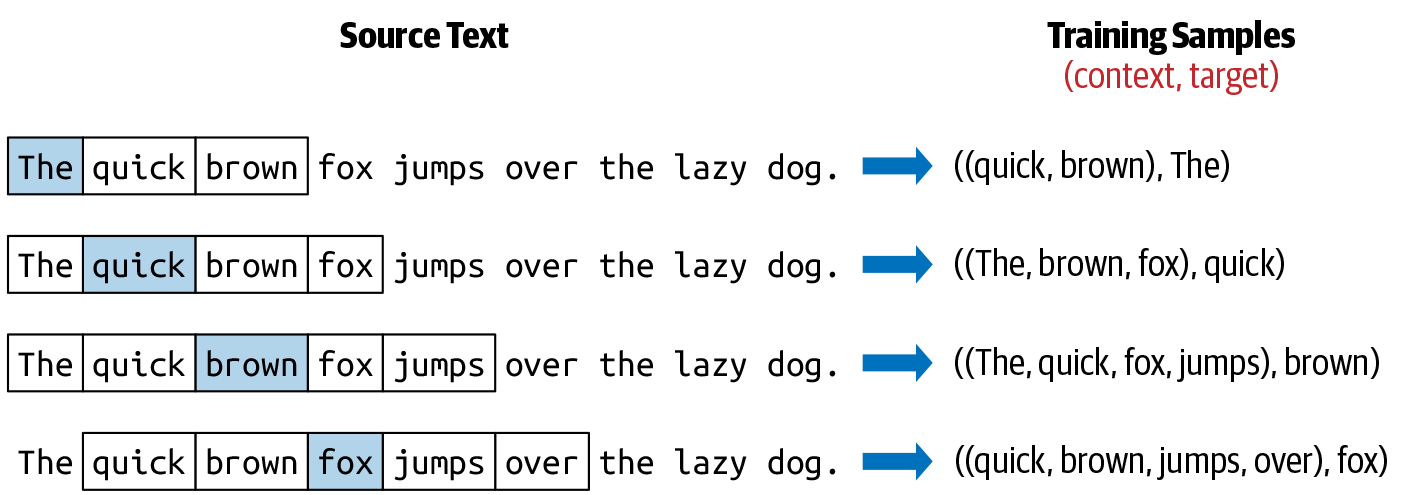
\includegraphics[width=0.65\textwidth]{capitulo3/figuras/nlp3.png}
	\caption{Preparando un conjunto de datos por CBOW
		\\\textit{Fuente: Extraído de} \protect\cite[p. 99]{vajjala2020practical}}
	\label{fig:nlp3}
\end{figure}

Cbow: Predice la palabra objetivo basándose en un contexto de palabras adyacentes, tomará cada palabra del corpus como palabra objetivo e intentará predecir la palabra objetivo a partir de sus palabras de contexto correspondientes. Por ejemplo, teniendo un tamaño de contexto dos (k=2), el  tamaño de la ventana deslizante será igual a 2k +1 donde uno representará  a la ventana central. Ver Figura \ref{fig:nlp3}



\begin{figure}[h!]
	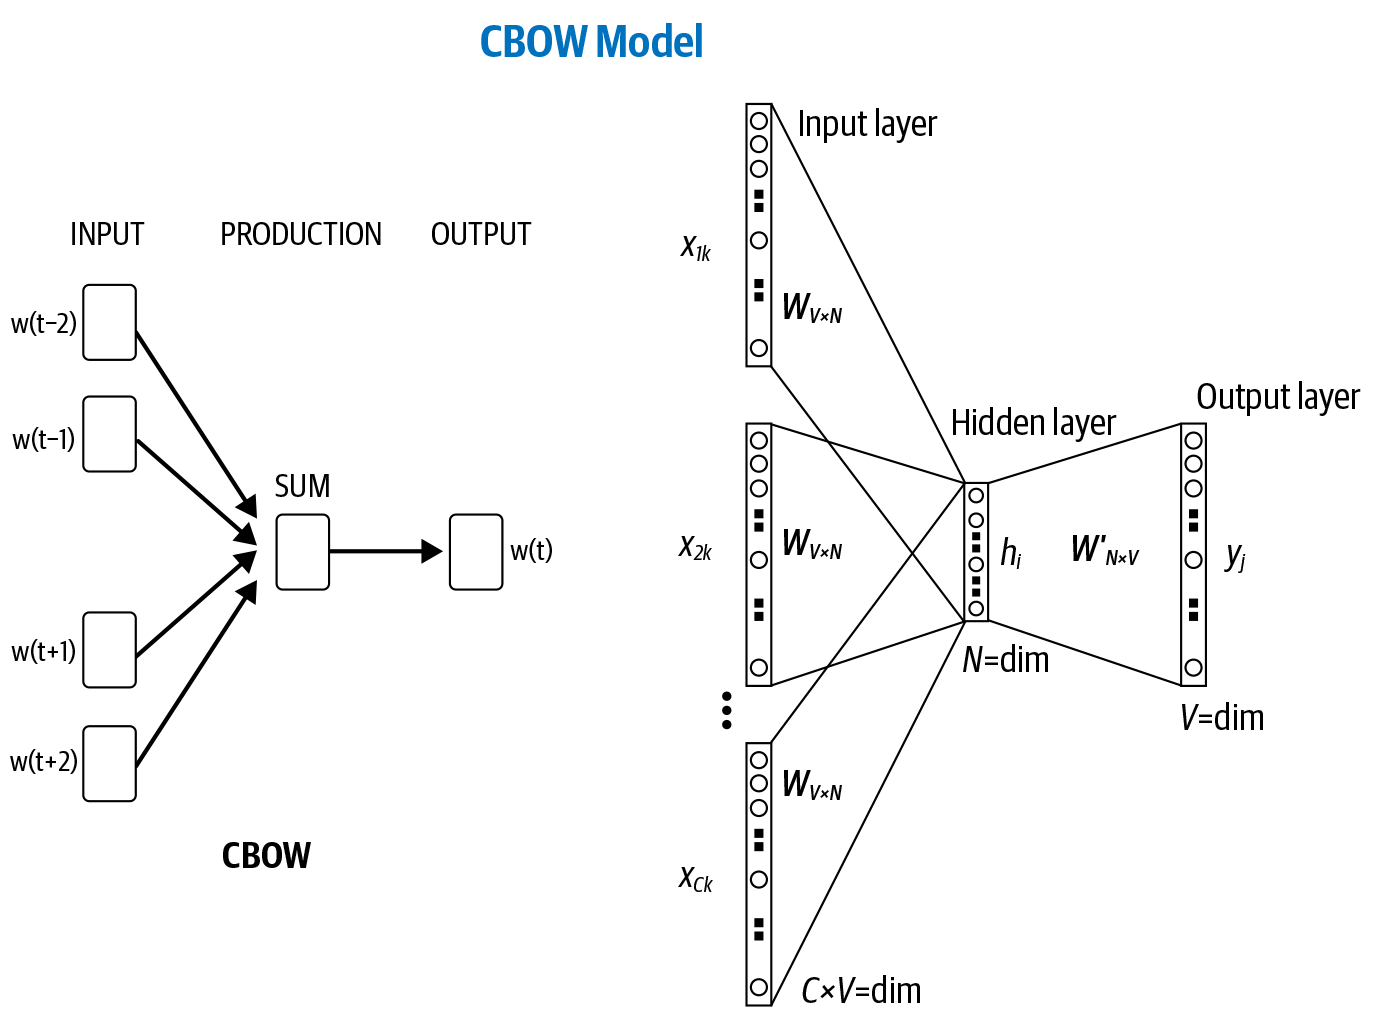
\includegraphics[width=0.65\textwidth]{capitulo3/figuras/nlp4.png}
	\caption{Modelo CBOW
		\\\textit{Fuente: Extraído de} \protect\cite[p. 100]{vajjala2020practical}}
	\label{fig:nlp4}
\end{figure}

El modelo Cbow utiliza una red neuronal poco profunda para aprender incrustaciones vectoriales de palabras. Esta red tiene una capa oculta y su objetivo es aprender una matriz de incrustación de palabras (definida como $E_{ \left | \textrm{V}  \right |\: \textrm{x} \: \textrm{d}}$,  donde $\left | \textrm{V}  \right | = $ tamaño del vocabulario, d= dimensión de incrustación)  a partir de un vocabulario (v)  dado inicialmente  \ref{fig:nlp4}. La matriz de incrustación se inicia de forma aleatoria. Posteriormente  la red selecciona vectores de las palabras del contexto de la matriz y los combina para generar un vector (d), que luego se multiplica con otra matriz ${E}'_{ \textrm{d} \: \textrm{x}  \:\left | \textrm{V}  \right | }$ en la siguiente capa. Esto da como resultado un vector de una dimensión por el tamaño del vocabulario ( $1 \times \left | \textrm{V}  \right |$) que funge como entrada para una función softmax para obtener la distribución de probabilidad en el espacio de vocabulario. Al final del entrenamiento, la matriz de incrustación $E$ y $E'$ obtenida se actualizan después de comparar la distribución aprendida con la etiqueta (palabra objetivo) mediante retropropagación.

\begin{figure}[h!]
	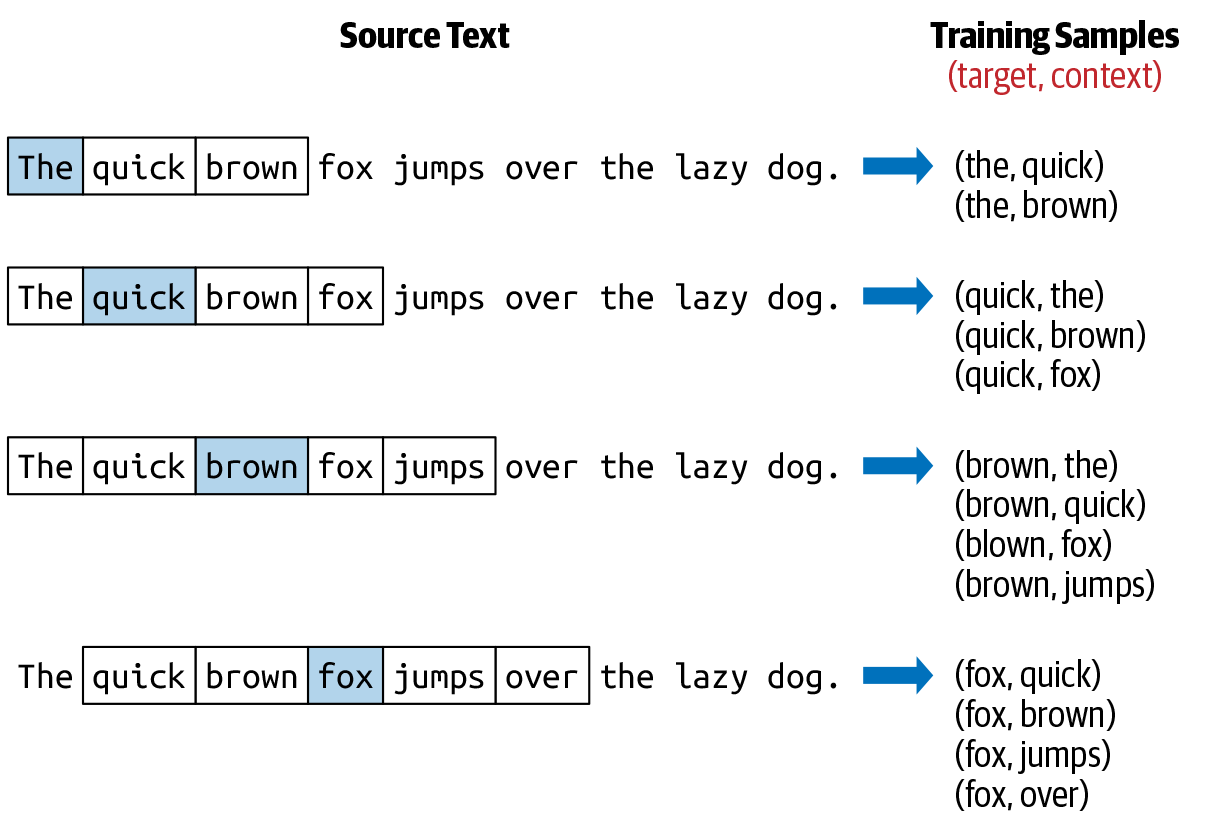
\includegraphics[width=0.6\textwidth]{capitulo3/figuras/nlp5.png}
	\caption{Preparando un conjunto de datos por SkipGram
		\\\textit{Fuente: Extraído de} \protect\cite[p. 101]{vajjala2020practical}}
	\label{fig:nlp5}
\end{figure}

Skip-gram: Predice las palabras del contexto a partir de la palabra central. Toma una palabra de entrada y predice las palabras que podrían aparecer en su contexto.``El conjunto de datos para entrenar un SkipGram se prepara de la siguiente manera: ejecutamos una ventana deslizante de tamaño 2k+1 sobre el corpus de texto para obtener el conjunto de 2k+1 palabras que están bajo consideración. La palabra central en la ventana es la X, y las k palabras a cada lado de la palabra central son Y'' \cite[p. 101]{vajjala2020practical}. Al igual que el modelo cbow, k representara el número de palabras, pero en este caso serán las que se deben predecir ver Figura \ref{fig:nlp5}



\begin{figure}[h!]
	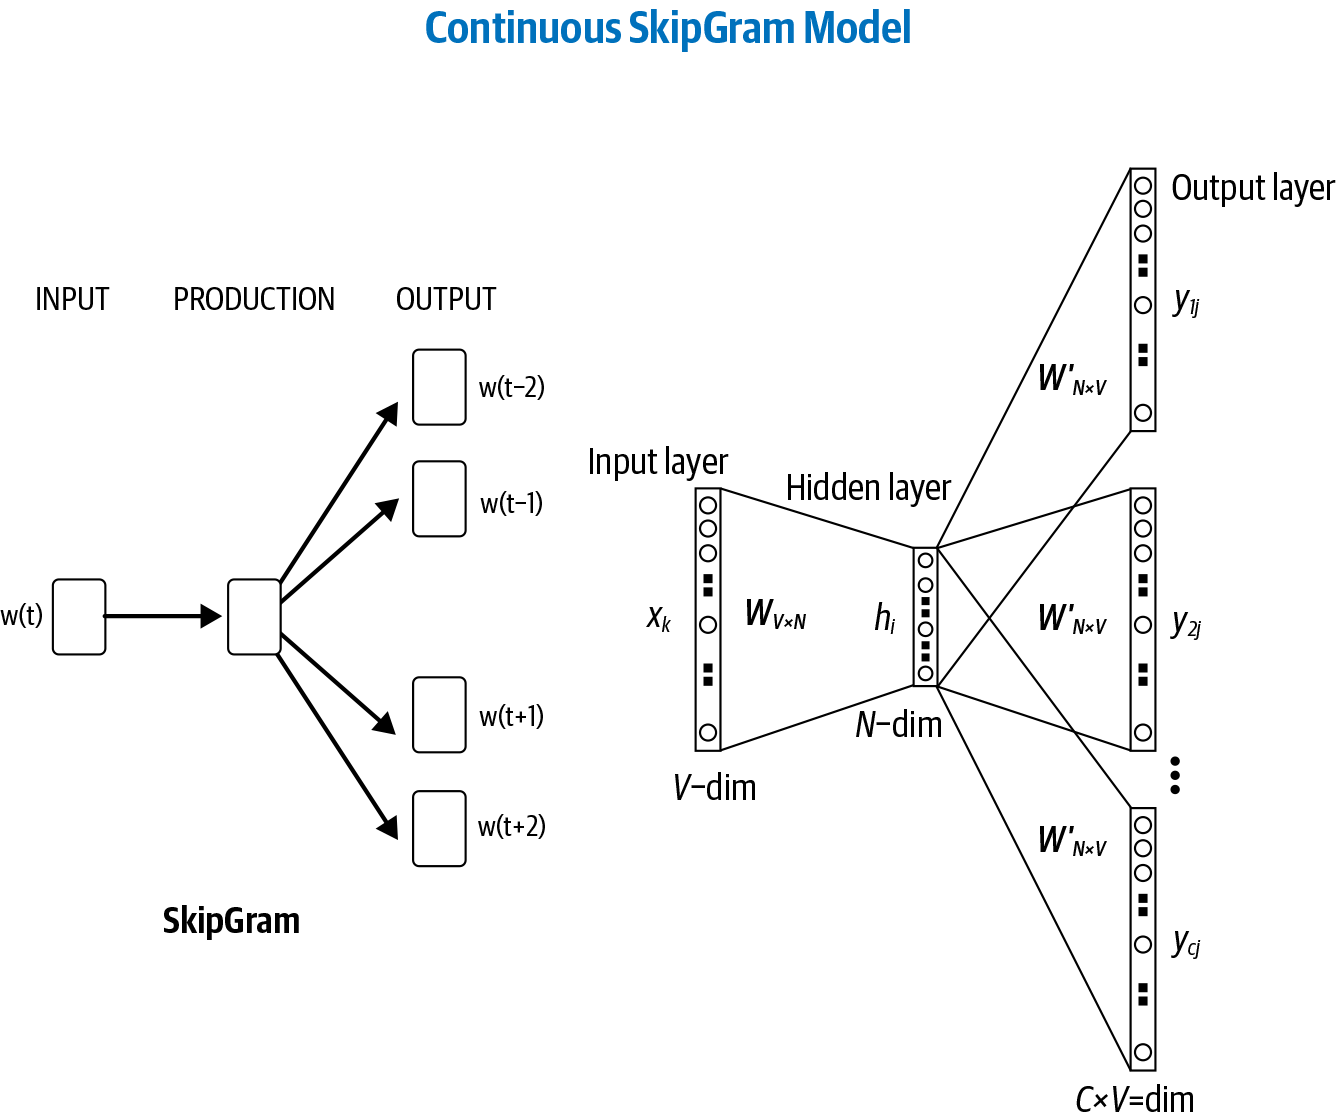
\includegraphics[width=0.65\textwidth]{capitulo3/figuras/nlp6.png}
	\caption{Modelo SkipGram
		\\\textit{Fuente: Extraído de} \protect\cite[p. 102]{vajjala2020practical}}
	\label{fig:nlp6}
\end{figure}

En el modelo SkipGram, se emplea una red similar a la usada en CBOW. En la capa de entrada, se toma el índice de la palabra objetivo para acceder a su vector correspondiente en la matriz de incrustación $E_{ \left | \textrm{V}  \right |\: \textrm{x} \: \textrm{d}}$,  donde $\left | \textrm{V}  \right | = $  , estos vectores se combinan y forman un nuevo vector que se multiplica por otra matriz ${E}'_{ \textrm{d} \: \textrm{x}  \:\left | \textrm{V}  \right | }$  para obtener un vector unidimensional de probabilidad en el espacio del vocabulario. La comparación entre esta distribución y la etiqueta se utiliza para actualizar las matrices de incrustación a través de la retropropagación. Al finalizar el entrenamiento, la matriz de incrustación obtenida (denotada como $E_{ \left | \textrm{V}  \right |\: \textrm{x} \: \textrm{d}}$) representara las palabras del vocabulario en vectores de baja dimensión.Ver Figura \ref{fig:nlp6}

	\item Word embeddings pre entrenados:  Son representaciones vectoriales de palabras generadas mediante modelos de lenguaje que han sido entrenados previamente con grandes cantidades de texto. Los embeddings pre entrenados más populares como wor2vec, glove y fastext que ya se mencionaron están disponibles para varias dimensiones como d = 25, 50, 100, 200, 300, 600. De igual forma, en muchas ocasiones, los investigadores comparten embeddings de palabras ya entrenados para ser utilizados libremente en proyectos académicos o comerciales. Cuando se opta por utilizar embeddings previamente entrenados, se tiene dos enfoques principales:
	
Estático: Implica emplear los embeddings tal como están, sin modificarlos. Esto es ideal si los embeddings se ajustan bien al problema y ofrecen buenos resultados.

Actualizado: Se basa en utilizar los embeddings pre entrenados para inicializar el modelo, pero se permite que se actualicen durante el entrenamiento. Esta opción puede ser beneficiosa si se busca integrar y mejorar el modelo en una tarea específica.

Si en estos modelos pre-entrenados no existieran representaciones vectoriales de palabras importantes para la tarea en cuestión, dependiendo de la librería en uso, se pueden reentrenar. 

Para decidir si reentrenar modelos previamente entrenados, una buena regla general es calcular la superposición de vocabulario. Si la superposición entre el vocabulario de nuestro dominio personalizado y el de las incrustaciones de palabras previamente entrenadas es superior al 80\%, las incrustaciones de palabras pre-entrenadas tienden a dar buenos resultados en la clasificación de texto.``Si la superposición entre el vocabulario del corpus y el vocabulario incorporado es inferior al 80\%, es poco probable que veamos un buen desempeño de nuestro modelo de PNL.''\cite[p. 104]{vajjala2020practical}.

	\item Oov y embeddings.- Abordar el problema de las palabras fuera del vocabulario en los modelos de embeddings es todo un desafío, ya que  las palabras fuera del vocabulario no tienen representaciones predefinidas, lo que dificulta su procesamiento y comprensión. Si se quiere rehusar embeddings pre entrenados para saltarse la difícil tarea de entrenar un embedding que requiere de miles y miles de datos para obtener una representación más o menos buena se debe considerar que las representaciones que se encuentren son suficientes y se adaptan al problema, o qué nuevas palabras deben añadirse. Para incorporar palabras nuevas a modelos que ya han sido entrenados, hay algunas estrategias que se pueden utilizar como:

El entrenamiento incremental: implica volver a ejecutar el algoritmo de entrenamiento con el corpus actualizado, que contiene las nuevas palabras. Esto puede ser costoso computacionalmente, en especial si el corpus es grande. 

Inicialización de vectores: Se pueden agregar palabras nuevas asignándoles vectores aleatorios o utilizando algún otro método de inicialización específico.``Una forma de lidiar con el problema OOV para incrustaciones de palabras es crear vectores que se inicializan aleatoriamente, donde cada componente está entre –0,25 y +0,25, y continuar usando estos vectores en toda la aplicación''\cite[p. 105]{vajjala2020practical}.

Sub-palabras: Modelos como FastText abordan el problema de OOV representando las palabras a través de sus constituyentes de caracteres, es decir, descomponiendo las palabras en n-gramas de caracteres (secuencias de caracteres de longitud n. En lugar de solo aprender incrustaciones de palabras completas, también aprende incrustaciones de n-gramas de caracteres. La representación de una palabra se construye agregando las incrustaciones de sus n-gramas de caracteres constituyentes.

Textos Completos:  Otro enfoque para lidiar con el problema OOV, es Doc2Vec. Es una técnica de aprendizaje no supervisado que genera representaciones vectoriales densas para documentos, lo que permite medir la similitud y realizar operaciones semánticas en documentos completos. ``es similar a Word2vec en cuanto a su arquitectura general, excepto que, además de los vectores de palabras, también aprende un ``vector de párrafo'' que representa el texto completo (es decir, con palabras en contexto).''\cite[p.106]{vajjala2020practical}. El vector de párrafo representa un texto completo (un párrafo, una oración o incluso un documento entero). 

Las redes neuronales superficiales utilizadas para aprender las incrustaciones de Doc2vec son parecidas a CBOW y SkipGram de Word2vec, el primer modelo se denomina memoria distribuida (DM) donde se integra tanto la información del contexto de palabras como la representación del documento completo para predecir la palabra objetivo. Esto permite que el modelo capture no solo el significado de las palabras individuales en un contexto, sino también la esencia general del documento en el que aparecen esas palabras. El segundo modelo se denomina bolsa de palabras distribuida (DBOW) este modelo omite la predicción de palabras y se centra únicamente en predecir el siguiente documento basándose solo en el vector de documento.
	
	\item Consideraciones.- A continuación se detallaran consideraciones importantes que tomar respecto al uso de embeddings pre entrenados:\\
Sesgo.-  Las representaciones de texto, como embeddings o vectores que capturan el significado de las palabras o textos, están influenciadas por los datos con los que se entrenan. Estos sesgos pueden tener impactos significativos en el rendimiento de los modelos que dependen de estas representaciones.\\

Exigencia computacional.- Los embeddings pre entrenados suelen ser archivos grandes, a menudo varios gigabytes. Este tamaño puede causar dificultades en el rendimiento si no se aborda adecuadamente. Por ejemplo, el modelo Word2vec requiere aproximadamente 4,5 GB de memoria RAM, lo que puede ser un desafío en ciertos escenarios.
\\
Representar necesidades.- Existen necesidades lingüísticas y de aplicación que van más allá de lo que las técnicas de embeddings pueden capturar actualmente. Por ejemplo, la detección de sarcasmo es una tarea que requiere matices y sutilezas que aún no son bien representadas o entendidas completamente mediante técnicas de embeddings.\\

Estado del arte.- La representación neuronal del texto es un área en constante evolución en el campo del procesamiento del lenguaje natural (PNL), con avances rápidos en el estado del arte. Aunque nuevos modelos suelen generar entusiasmo, es importante considerar aspectos prácticos, usar modelos nuevos no siempre será la mejor opción, es importante considerar que también se pueden tener buenos resultados con modelos de embeddings básicos, que además no requieren de mucha capacidad computacional. 

\end{itemize}
\end{itemize}




\section{DEEP LEARNING PARA LA CLASIFICACIÓN DE TEXTO}
Al trabajar con redes neuronales, se requiere un procesamiento adicional de los vectores de entrada para adaptarlos a las capas de entrada de la red neuronal. Estos pasos describen la preparación de datos para usarlos como entrada en una arquitectura de red neuronal en el contexto del procesamiento de lenguaje natural. Si bien estos pasos ya se mencionaron anteriormente es importante resaltarlos ya que son fundamentales para preparar datos textuales, debido a que transforman los textos en representaciones numéricas adecuadas que pueden ser entendidas y procesadas por la red neuronal.

\begin{itemize}

	\item Tokenización: Consiste en dividir los textos en unidades más pequeñas, como palabras o subpalabras (tokens).
	
	\item Conversión a vectores de índices de palabras: Asigna un número único a cada palabra o token del texto.

	\item Relleno de secuencias de texto para tener la misma longitud: En muchos modelos de redes neuronales, todas las secuencias deben tener la misma longitud. Si las secuencias de texto tienen longitudes diferentes, se pueden rellenar con valores específicos (como 0) para que todas tengan la misma longitud. Por ejemplo, si el máximo de palabras permitidas es 100 y un texto tiene 80 palabras, se pueden agregar 20 valores de relleno al final.
	
	\item Asignación de índices de palabras: Cada índice de palabra (número único) se asigna a un vector de incrustación correspondiente. Se multiplican los vectores índice de palabras con la matriz de incrustación para obtener vectores de incrustación asociados a cada palabra en el texto.
	
	\item Uso del resultado como entrada: Los vectores de incrustación resultantes, que representan las palabras de los textos y están listos para ser procesados por la red neuronal, se utilizan como la entrada para la arquitectura de la red neuronal.

\end{itemize}

\section{LAS REDES SOCIALES Y EL PLN}
El texto extraído de las redes sociales presenta desafíos y problemas específicos debido a la naturaleza única de estos datos. Algunos de los problemas comunes son:

\begin{itemize}

	\item Ruido y calidad del texto: Los datos de redes sociales suelen contener errores ortográficos, abreviaturas desenfrenadas, emojis, jerga, sarcasmo, uso  de mayúsculas inconsistentes, repetición de caracteres y lenguaje informal. Las conversaciones en especial en las redes sociales no siguen ninguna gramática, además de tener contenido irrelevante como propaganda.``Las publicaciones en las redes sociales están llenas de spam, anuncios, contenido promocionado y todo tipo de contenido no solicitado, irrelevante o que distrae''\cite[p. 283]{vajjala2020practical}. Esto puede dificultar la comprensión y el análisis del texto, ya que requiere un preprocesamiento más cuidadoso para lidiar con estas peculiaridades.
	
	\item Variabilidad lingüística y diversidad de idiomas: Las redes sociales son utilizadas a nivel mundial, lo que significa que los datos provienen de una amplia gama de idiomas y dialectos. Esta variabilidad lingüística agrega complejidad al procesamiento de texto y a la construcción de modelos que funcionen adecuadamente en diferentes idiomas.
	
	\item Vocabulario en constante evolución.- Las redes sociales son semilleros para la creación de nuevos términos y modismos que pueden volverse virales rápidamente. ``cuando se trata del lenguaje social, el vocabulario aumenta a un ritmo muy rápido. Cada día aparecen nuevas palabras. Esto significa que cualquier sistema de PNL que procese SMTD ve muchas palabras nuevas que no formaban parte del vocabulario de los datos de entrenamiento''. \cite[p. 281]{vajjala2020practical}. Los modelos de PLN deben ser capaces de adaptarse rápidamente a estos cambios en el vocabulario. La actualización constante de estos modelos para capturar nuevos términos y usos del lenguaje se vuelve esencial para mantener la eficacia en la comprensión de texto en entornos de redes sociales.
	
	\item Ambigüedad y contexto: Los mensajes en redes sociales pueden carecer de contexto, lo que lleva a ambigüedad en el significado. La falta de contexto puede dificultar la interpretación precisa del texto, especialmente en el caso de ironías, dobles sentidos o mensajes sarcásticos.	
\end{itemize}

\begin{figure}
	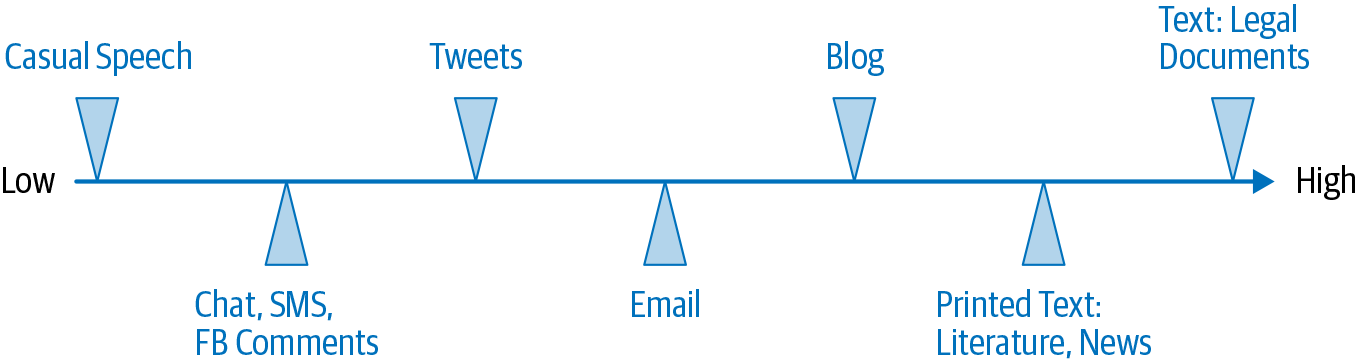
\includegraphics[width=0.65\textwidth]{capitulo3/figuras/nlp7.png}
	\caption{Espectro de formalismo en textos según sus fuentes}
	\floatfoot{Fuente: Practical natural language processing: A comprehensive guide to building real-world NLP systems \cite[p. 283]{vajjala2020practical} }
	\label{fig:nlp7}
\end{figure}

Los datos textuales provenientes de redes sociales tienden a ser considerablemente más informales en comparación con textos provenientes de blogs, libros, artículos de noticias o documentos legales.

 La Figura \ref{fig:nlp7} ilustra el espectro de formalidad en los datos de texto, ubicando diferentes fuentes de datos textuales dentro de este espectro.



Es esencial comprender la distinción entre el procesamiento de texto formal y el extremadamente informal, como el que se encuentra en las redes sociales. La labor de limpieza en este último caso debe ser más minuciosa: implica revisar exhaustivamente el texto para identificar qué aspectos se deben limpiar y qué herramientas o funciones adicionales se deben implementar para eliminar las particularidades presentes. Se requiere una cantidad significativa de tiempo y esfuerzo humano para dejar el texto en condiciones utilizables para las fases posteriores. Se hace un énfasis al esfuerzo humano debido a que el uso de herramientas existentes para el texto de redes sociales probablemente no den resultados tan satisfactorios. Estas herramientas están diseñadas para operar de manera más general y no específicamente adaptadas para manejar las características únicas que se pueden encontrar en este tipo de texto tan dinámico.
\section{CONJUNTOS DE DATOS RELACIONADOS CON EL LENGUAJE OFENSIVO}
Existen diversos conjuntos de datos relacionados con el lenguaje ofensivo extraídos de distintas redes o plataformas sociales. Muchos de estos conjuntos se encuentran mayormente en inglés, como el conjunto de datos ``Hate Speech and Offensive Language'' disponible públicamente en Kaggle, mismo que contiene mensajes recopilados de la red social Twitter. Este conjunto de datos alberga 2,458,155 tweets publicados por usuarios que expresan odio.

Encontrar conjuntos de datos en español es un desafío, uno de los pocos conjuntos disponibles es ``Offendes'', enfocado en influencers jóvenes de plataformas sociales como Twitter, Instagram y YouTube. Este corpus recopilado está compuesto por comentarios en español etiquetados manualmente como: ofensivos, dirigidos a un individuo específico (OFP); ofensivos, dirigidos a grupos basados en etnia, género, orientación sexual, ideología política, creencia religiosa u otras características comunes (OFG); no ofensivos pero con lenguaje grosero (NOE), y finalmente, no ofensivos (NO). El conjunto de datos público de Offendes contiene 30,416 muestras seleccionadas el total usado en la tarea ``MeOffendes'' en el IberLEF 2021. El IberLEF (Iberian Languages Evaluation Forum) es un espacio de evaluación que se enfoca en los desafíos y avances del procesamiento de lenguaje natural para las lenguas ibéricas, incluyendo el español, portugués y otras lenguas regionales como el catalán y el gallego.

Offendes se divide en tres subconjuntos: entrenamiento con 16,710 muestras, desarrollo con 100 muestras y prueba con 13,606. Para un detalle más específico sobre la cantidad de datos etiquetados, ver la tabla \ref{tbl:13}. Este conjunto de datos se usará con el fin de ayudar en el etiquetado de los datos recopilados y además para tener más variabilidad en los datos.

\begin{table}[!ht]
	\centering
	\begin{tabular}{|c|c|c|c|}
		\hline
		\textbf{Label} & \textbf{Training} & \textbf{Development} & \textbf{Test} \\ \hline
		NO & 13212 & 64 & 9651 \\ 
		NOE & 1235 & 22 & 2340 \\ 
		OFP & 2051 & 10 & 1404 \\ 
		OFG & 212 & 4 & 211 \\ \hline
		\textbf{Total} & 16710 & 100 & 13606 \\ \hline
	\end{tabular}
	\caption{Detalle distribucion categorias OffendES}
	\label{tbl:13}
\end{table}


\section{CREACIÓN DEL CONJUNTO DE DATOS RELACIONADO CON EL LENGUAJE OFENSIVO EN EL CONTEXTO BOLIVIANO}
El conjunto de datos utilizado en este proyecto fue recopilado exclusivamente de dos plataformas de redes sociales: Facebook y WhatsApp. Se extrajo una cantidad significativa de muestras, las cuales fueron sometidas a un exhaustivo proceso de preprocesamiento y análisis. Durante este proceso, se realizaron diversas operaciones de limpieza para garantizar la calidad y relevancia de los datos.

Como resultado de estas operaciones de limpieza, las cifras originales de muestras variaron. A continuación, se presentan dos tablas que resumen este proceso: La tabla 1 muestra la cantidad inicial de comentarios extraídos, incluyendo aquellos que contenían enlaces, duplicados y contenido no relevante, entre otros aspectos. La tabla presenta la cantidad final de comentarios considerados útiles después de haber sido sometidos al proceso de limpieza. Se eliminaron duplicados y se aplicaron filtros para garantizar la calidad y relevancia de los datos.

tabla 1
-------------------------------------------------------------
cifras originales de comentarios extraidos:
Conjunto de datos
Santa Cruz   16380
La Paz          15861
Cbba             38913
WhatsApp     20826
total comentarios 91980
cifras finales despues de la limpieza
---------------------------------------------------------------

tabla 2
-----------------------------------------------------------
Conjunto de datos
Santa Cruz  14385
La Paz 14229
Cbba 35863
WhatApp 14501
total comentarios 78978
-----------------------------------------------------------

Los comentarios cuyas cifras han sido presentadas en las tablas anteriores fueron cuidadosamente seleccionados para reflejar la diversidad y riqueza de la comunicación en cada uno de los nueve departamentos de Bolivia. Estos departamentos están divididos en tres regiones distintas: el altiplano, que incluye La Paz, Oruro y Potosí; los valles, que abarcan Chuquisaca, Cochabamba y Tarija; y los llanos, que comprenden Santa Cruz, Pando y Beni.

Esta selección se llevó a cabo considerando variantes existentes en el uso del idioma español en cada región del país. Además, se decidió focalizar en un departamento específico de cada zona debido a la distribución demográfica característica de cada uno. Por ejemplo, los departamentos de Santa Cruz, La Paz y Cochabamba albergan la mayor cantidad de habitantes en sus respectivas regiones, lo que los convierte en representantes significativos de la diversidad lingüística y cultural de Bolivia.



\subsection{Palabras clave y elección de comentarios}
A continuación se brindarán detalles sobre la recolección de comentarios en las redes sociales de facebook y whatsapp.

\textbf{Facebook}

Todos los comentarios de la red social Facebook fueron extraídos de forma manual, empleando palabras o frases clave durante la búsqueda de las publicaciones correspondientes. Esta práctica se llevó a cabo debido a la falta de un control sobre la ubicación geográfica de las publicaciones en Facebook. A continuación se presentan las palabras clave seleccionadas:
\begin{itemize}
	\item racista /racismo
	\item sexista/sexismo
	\item homosexual/homofobia/homofobico
	\item lenguaje ofensivo/lenguaje de odio 
	\item discriminar/discriminacion
	\item machista/machismo
	\item violento/violencia
	\item feminista/feminismo  
\end{itemize}
y los nombres de las ciudades de Bolivia que se usaron conjuntamente con cada uno de las palabras clave en la búsqueda para encontrar comentarios ofensivos en la red social facebook:
\begin{itemize}
	\item Cochabamba
	\item Santa Cruz
	\item La Paz
	
\end{itemize}

Además de utilizar palabras clave para identificar publicaciones relevantes para este proyecto, también se llevó a cabo la selección de perfiles de autoridades políticas, medios de información y medios de comunicación en Bolivia. Esto se hizo con la comprensión de que los temas políticos y los hechos relevantes del país siempre han sido de gran interés para la población boliviana. Es en estos perfiles donde las personas tienden a concentrar sus opiniones y expresar sus desacuerdos de manera más frecuente. Para mas detalles ver tabla \ref{tbl:16}.


\begin{table}[!ht]
	\centering
	\begin{tabular}{|c|c|}
		\hline
		\textbf{Tipo de perfil} & \textbf{Nombre de Perfiles} \\ \hline
		Figuras politicas del pais  & \makecell{Evo Morales Ayma, Luis Fernando Camacho, \\  Andronico Rodriguez} \\ \hline
		Periódicos digitales                       & El Deber, Los tiempos, Pagina siete \\ \hline
		Canales de television & Unitel, Atb, Bolivision \\ \hline
		Radio  & Radio Qhana, Radio Sonar \\ \hline
		Otros medios de comunicacion & Sport Bolivia, Mi bolivia Plurinacional \\ \hline
		~ & ~ \\ \hline
	\end{tabular}
	\caption{Detalle perfiles para extraccion de comentarios}
	\label{tbl:16}
\end{table}

\textbf{Whatsapp}


Para recolectar los comentarios de la aplicación de mensajería WhatsApp, se eligió un grupo de chat compuesto por 7 miembros jóvenes, con edades comprendidas entre los 21 y 27 años, que habitualmente se comunicasen de manera brusca, grosera y/o ofensiva. Esta selección se realizó con el consentimiento del administrador del grupo, quien exportó el chat directamente desde WhatsApp en un documento con extensión .txt. Posteriormente, el archivo fue sometido a un proceso exhaustivo de limpieza y preprocesamiento de datos, los detalles de la limpieza y la clasificación de los mismos se detallaran más  adelante.

\subsection{BERT y el etiquetado de comentarios}
Durante la revisión del conjunto de datos "Offendes", se identificó que existian varias muestras que requerían reetiquetado, especialmente aquellas marcadas con lenguaje grosero. Por lo tanto, se revisó nuevamente todo el conjunto de datos, centrándose especialmente en las muestras con lenguaje grosero, y se procedió a reetiquetar manualmente teniendo en cuenta su utilidad y la percepción sobre si estos comentarios pertenecian a la categoria de groseros, ofensivos o no ofensivos en la sociedad boliviana. Este proceso se abordó detalladamente en el capítulo 4 del proyecto.

De un total de 30,416 comentarios, 2,310 pertenecían a la clase de comentarios groseros pero no ofensivos. Se reetiquetaron 142 comentarios de esta clase y posteriormente se llevó a cabo la limpieza de este conjunto de datos para su uso adecuado.

El etiquetado de los conjuntos de datos de Facebook y WhatsApp se realizó después de la limpieza de los mismos. Para esta tarea, se utilizó la técnica de aprendizaje por transferencia, que consiste en aprovechar los conocimientos adquiridos en una tarea para mejorar el rendimiento en otra tarea relacionada pero diferente. En este caso, se empleó el dataset ``Offendes'' para afinar una versión reducida del modelo BERT, el cual fue inicialmente entrenado con grandes cantidades de texto no etiquetado, como páginas web, libros y artículos de noticias.

A través de este proceso de entrenamiento masivo, el modelo aprende a comprender la estructura y el significado del lenguaje natural de manera general. Por lo tanto, cuando se adapta o afina para tareas específicas, como la clasificación de comentarios ofensivos, el modelo ya posee un conocimiento previo considerable del lenguaje, lo que permite mejorar su rendimiento en la tarea objetivo. Esto permitió que una muestra de aproximadamente 30,000 comentarios previamente etiquetados fuera utilizada para etiquetar los más de 78,000 comentarios recopilados de las redes sociales.

Bert

BERT, que significa Bidirectional Encoder Representations from Transformers, es un modelo de lenguaje pre entrenado desarrollado por Google, tiene una arquitectura compuesta por múltiples capas de transformers, que son unidades básicas que procesan secuencias de entrada de manera bidireccional. Esto significa que el modelo puede capturar el contexto de una palabra en una oración teniendo en cuenta tanto las palabras que la preceden como las que la siguen, lo que lo hace extremadamente efectivo para una amplia gama de tareas de procesamiento del lenguaje natural. Esto se logra mediante el entrenamiento del modelo en dos tareas: 

1.- El modelado de lenguaje enmascarado (Masked Language Modeling, MLM) que ocurre durante el entrenamiento, donde BERT recibe una secuencia de palabras de entrada y algunas de estas palabras son enmascaradas aleatoriamente. La tarea del modelo es predecir qué palabra falta en cada lugar enmascarado, lo que obliga al modelo a comprender el contexto de las palabras en una oración para poder predecir la palabra enmascarada con precisión. Ver figura 1

2.- Predicción de la siguiente oración: Además del MLM, BERT también se entrena en una tarea de predicción de la siguiente oración. Se le proporcionan dos oraciones y el modelo debe predecir si la segunda oración sigue a la primera en un contexto coherente o no.


----------------------------------------------
figura 1

-----------------------------------------------

 Resultados del etiquetado con Bert

Inicialmente, se utilizó el conjunto de datos "Offendes" para entrenar y afinar  el modelo BERT seleccionado, con el fin de etiquetar posteriormente el conjunto de datos recolectado de la región de los valles, centrándose específicamente en el departamento de Cochabamba. Los resultados del entrenamiento de BERT con "Offendes" se pueden apreciar en la Tabla "algo1", donde en cantidad de muestras se detalla la cantidad de comentarios usados para el conjunto de entrenamiento, validación y prueba, en precisión la exactitud del modelo en su respectivo conjunto y en error las etiquetas que se marcaron incorrectamente en cada conjunto.

------------------------------------
tabla algo 1

------------------------------------

Bajo el resultado obtenido descrito en la Tabla algo1, se etiquetó el conjunto de datos de Cochabamba, cuyos resultados se detallan en la Tabla "algo2", donde la precisión es el resultado de la revisión manual realizada después del etiquetado. Finalmente despues de todo este proceso se etiquetaron los tres últimos conjuntos de datos restantes. En la tabla 3 se pueden observar los resultados del etiquetado del conjunto de datos de Santa Cruz, en la tabla 4 se presentan los resultados obtenidos para el conjunto de datos de La Paz, y finalmente, en la tabla 5 se muestran los resultados obtenidos para el conjunto de datos de WhatsApp.


-------------------------------------

tabla algo 2

------------------------------------
---------------------------------

tabla algo 3

-------------------------------

---------------------------------

tabla algo 4

--------------------------------
-----------------------------

tabla algo 5

------------------------------




\subsection{División de comentarios para el entrenamiento}
Se trabajó con una porción del conjunto de datos total, específicamente con 35,000 muestras, las cuales se dividieron en tres partes: el conjunto de entrenamiento, el conjunto de prueba y el conjunto de validación. Las proporciones correspondientes a cada porción se pueden visualizar en la tabla \ref{tbl:conjuntos}, para asegurar la uniformidad en la distribución de clases, lo cual es crucial para el rendimiento del modelo, se creó este conjunto de datos priorizando una cantidad de muestras equilibrada para cada clase.


\begin{table}[!ht]
	\centering
	\begin{tabular}{|c|c|c|c|c|}
		\hline
		\textbf{Conjunto} & \textbf{Ofensivo} & \textbf{No ofensivo} & \textbf{Grosero} & \textbf{Porcentaje (\%)} \\ \hline
		Entrenamiento & 10250 & 10250 & 4000 & 24500 = 70\% \\ 
		Validación & 2125 & 2125 & 1000 & 5250 = 15\% \\ 
		Prueba & 2580 & 2572 & 98 & 5250 = 15\% \\ \hline
		\textbf{Total} & 14955 & 14947 & 5098 & \textbf{35.000 = 100\%} \\ \hline
	\end{tabular}
	\caption{División del conjunto de datos}
	\label{tbl:conjuntos}
\end{table}


Como se puede observar en la tabla 3.10 la cantidad de clases en los conjuntos de datos no es uniforme para la categoría de lenguaje grosero, esto debido a que la cantidad de muestras totales para esta categoría no sobrepasa los 6000 ejemplares y por esa razón se priorizo otorgarle la mayor cantidad de muestras posibles a los conjuntos de entrenamiento y validación.







\chapter{LENGUAJE OFENSIVO EN BOLIVIA}\label{chp-diseno}
En este capítulo, se explorará en detalle el concepto de lenguaje ofensivo, su definición y sus diversas manifestaciones. Se analizará cómo el lenguaje ofensivo puede tener un impacto en la comunicación, las relaciones interpersonales y la sociedad en general. Además, se contextualizará específicamente en el ámbito de Bolivia, considerando su diversidad cultural y social.

\section{ DEFINICIÓN Y CARACTERÍSTICAS DEL LENGUAJE OFENSIVO}
En esta sección, se explorarán algunas definiciones y caracterizaciones que han surgido a lo largo del tiempo para capturar la esencia de la forma de comunicación ofensiva. Además, se examinarán las principales características que definen y distinguen al lenguaje ofensivo, haciendo hincapié en su impacto emocional y social en aquellos que lo encuentran o lo reciben.
\subsection{Definición de lenguaje ofensivo}
En la actualidad, se encuentran bastantes diferencias terminológicas para referirse a lo que se puede considerar lenguaje ofensivo, si bien ofensivo, es el término que se decidió adoptar para fines de este proyecto, en distintos estudios lingüísticos, se ha abordado este tipo de lenguaje bajo otras denominaciones como ``lenguaje sucio'', ``lenguaje fuerte'', ``lenguaje soez'', ``lenguaje tabú'', ``lenguaje grosero'', ``lenguaje cargado de emociones'', entre otros.
Se presentan dos definiciones para ilustrar la variedad de enfoques sobre este tipo de lenguaje:

``Cualquier palabra o cadena de palabras que tiene o puede tener un impacto negativo en el sentido de sí mismo y/o el bienestar de aquellos que se encuentran con ella, es decir, hace o puede hacer que se sientan leve o extremadamente desconcertados y/o insultados y/ o heridos y/o asustados'' \cite[p. 16]{o2020offensive}.


``El lenguaje ofensivo se refiere a aquellos términos lingüísticos o expresiones compuestas por palabrotas, maldiciones, etc., que normalmente se consideran despectivos y/o insultantes.''\cite[p. 28]{avila2016treatment}.

Estas definiciones representan solo un fragmento de las diversas interpretaciones que existen. Es esencial notar que, independientemente del enfoque adoptado para definir este tipo de lenguaje, todos resaltan su característica principal: su negatividad general percibida por aquellos que lo leen o escuchan.



\subsection{Definición de lenguaje ofensivo en Bolivia}
El diputado Juan José Huanca Mamani presentó el proyecto de ley fechado el 1 de marzo de 2023, titulado ``Proyecto de Ley que regula y sanciona el uso indebido de las redes sociales en todo el territorio del Estado Plurinacional de Bolivia''. Esta propuesta detalla disposiciones legales específicas para regular el uso problemático de las redes sociales en el país. Aunque el proyecto no se enfoca de manera individual en el lenguaje ofensivo en las plataformas, aborda principios generales fundamentales.

En el artículo 3 sobre principios generales, se resalta la importancia del respeto hacia terceras personas en el entorno de las redes sociales: ``En el uso de las redes sociales en sus diferentes ámbitos, se debe tener presente el respeto hacia las terceras personas en un espacio amplio de navegación vía internet, donde cada usuario tiene su propia opinión, que no siempre se debe compartir, pero sí respetar'' \cite[Articulo 3, PL. 304 2022-2023]{diputados2023ley}.

El artículo 6 establece restricciones claras, prohibiendo la publicación de información, comentarios, imágenes o videos ofensivos, amenazantes o que afecten la imagen personal, la honra, la intimidad, la integridad personal o la libertad de expresión en internet. También prohíbe el uso de un lenguaje violento que incite al odio o la discriminación en formas prohibidas por la ley \cite[Articulo 6, PL. 304 2022-2023]{diputados2023ley}.

Los artículos 8 y 9 establecen las sanciones para quienes atenten contra la dignidad y el honor de otros a través de las redes sociales, con penas que pueden llegar a una privación de la libertad de entre cinco y siete años.
Aunque el proyecto no define términos clave como ``ofensivo'' o ``violento'', se evidencia la intención de no tolerar conductas que involucren este tipo de comportamientos en las redes sociales \cite[Articulo 3, PL. 304 2022-2023]{diputados2023ley}.

\subsection{Características del lenguaje ofensivo}
Las características del lenguaje abarcan un amplio espectro de elementos que definen la naturaleza y la función de la comunicación humana. La lingüística es la disciplina dedicada al estudio científico del lenguaje. Se enfoca en entender cómo se estructuran, funcionan y se utilizan los distintos sistemas de comunicación humana, ya sea oral, escrito o gestual. La lingüística abarca diversas áreas de estudio, como la morfología, la sintaxis, la semántica, entre otras importantes ramas.  Es por esa razón que se detallara a continuación el área de estudio de cada una y su relación con el lenguaje ofensivo:

Sociolingüística del lenguaje ofensivo. La sociolingüística es una rama de la lingüística que se centra en el estudio de la relación entre el lenguaje y la sociedad. ``La linguistica y la sociologia establecen relaciones entre los usos y actitudes linguisticas de una sociedad donde coexisten lenguas, razas y culturas completamente complejas y en el que las personas dependen unas de otras reciprocamente presuponiendo relaciones y conflictos. Se considera a la lengua y a la sociedad unidos, ambos, no pueden ser considerados aisladamente al margen de la ``cultura''.'' \cite{prado2004analisis}.

El uso de lenguaje ofensivo está influenciado por factores sociales, como la cultura, la identidad, la jerarquía social y las actitudes hacia ciertos grupos o individuos. Aquí hay algunas características sociolingüísticas del lenguaje ofensivo:

\begin{itemize}
		\item Variación según contextos sociales.- El lenguaje ofensivo puede variar según el contexto social y cultural en el que se utilice. Las palabras o expresiones que se consideran ofensivas en un entorno pueden no serlo en otro, dependiendo de las normas y las actitudes lingüísticas de esa comunidad.
		\item Jerarquía y poder.-  El lenguaje ofensivo a menudo refleja relaciones de poder y jerarquía. Puede utilizarse para denigrar a grupos o individuos que se perciben como menos poderosos o marginados en una sociedad.
		\item Efectos en la percepción social.- El uso de lenguaje ofensivo puede influir en la percepción social y en cómo se ven y se tratan ciertos grupos. Puede reforzar estereotipos negativos y contribuir a la discriminación. 
		\item Cambios en las actitudes lingüísticas.- Las actitudes hacia el lenguaje ofensivo pueden cambiar con el tiempo debido a cambios culturales y sociales. Lo que se consideraba aceptable en el pasado puede ser considerado inaceptable en el presente o igualmente de forma contraria.
		\item Códigos y contextos informales.- El lenguaje ofensivo a menudo se encuentra en contextos informales, como conversaciones entre amigos o en interacciones en línea. Esto puede reflejar la relajación de las normas lingüísticas en contextos menos formales.

\end{itemize}

Pragmática del lenguaje ofensivo. La pragmática es un campo de estudio lingüístico que se enfoca en el significado del lenguaje en contexto, es decir va más allá de la estructura formal de las palabras y oraciones. Como expresa \citeA{dascal1999pragmatica} La pragmática es el estudio del uso de los medios lingüísticos a través de los cuales un hablante dirige sus intenciones comunicativas y un oyente las reconoce.
	
La pragmática en el lenguaje ofensivo implica analizar cómo se interpreta las expresiones ofensivas en contextos de comunicación. Considerar los aspectos pragmáticos es esencial para comprender por qué y cómo se emplea el lenguaje ofensivo en diferentes situaciones y cómo afecta a la interacción comunicativa. Algunos aspectos pragmáticos relacionados con el lenguaje ofensivo incluyen:

\begin{itemize}
		\item Implicaturas y significado indirecto.- El lenguaje ofensivo a menudo utiliza implicaturas conversacionales, donde el significado implícito de una expresión va más allá del significado literal. Los hablantes pueden emplear el lenguaje ofensivo de manera indirecta para transmitir su intención ofensiva sin usar un lenguaje explícitamente vulgar.
		
		\item Contexto y relación.- La interpretación del lenguaje ofensivo depende del contexto de la comunicación y de la relación entre los interlocutores. Lo que puede ser ofensivo para un oyente puede no serlo para otro, dependiendo de la familiaridad y la percepción mutua entre las partes.
		
		\item Intención y efecto.- La interpretación del lenguaje ofensivo a menudo involucra analizar tanto la intención del hablante como el efecto que el mensaje tiene en el receptor. La percepción de la intención puede variar, y el lenguaje ofensivo puede tener diferentes efectos emocionales y psicológicos en diferentes personas.
		
		\item Atenuación y refuerzo.- Los hablantes pueden utilizar estrategias pragmáticas para atenuar o reforzar el impacto del lenguaje ofensivo. Por ejemplo, el uso de sarcasmo puede atenuar el impacto negativo o, por el contrario, reforzar la ofensa al comunicar una actitud despectiva.
\end{itemize}

Dialectología en el lenguaje ofensivo. La dialectología es una rama de la lingüística que se ocupa del estudio de los dialectos. Los dialectos son variedades de una lengua que difieren en aspectos fonéticos, gramaticales, léxicos y hasta pragmáticos, y pueden variar de una región a otra, dentro de un país o incluso entre países. ``La Dialectologia, rama de la linguistica, se ocupa de estudiar la variacion linguistica dentro de una sociedad, el habla de cada dia que no tiene cultivo literario y que ademas es propio de cada individuo, tomando en cuenta su diferenciacion o realidad que puede escaparse del esquema de cualquier norma y producir el cambio linguistico tanto en forma como en significado'' \cite[p. 20]{prado2004analisis}.

La dialectología en el contexto del lenguaje ofensivo se refiere al estudio de cómo las variaciones dialectales influyen en la forma en que se emplea y se interpreta el lenguaje ofensivo en diferentes regiones o comunidades lingüísticas. Aquí hay algunas consideraciones específicas de la dialectología en relación con el lenguaje ofensivo:

\begin{itemize}
			\item Tabúes y eufemismos: Las variaciones dialectales también pueden influir en cómo se tratan los tabúes lingüísticos y el uso de eufemismos. Algunas palabras ofensivas pueden ser reemplazadas por términos menos ofensivos en ciertos dialectos, mientras que en otros dialectos pueden mantenerse sin censura.
			
			\item Influencia en la intensidad: Algunos dialectos pueden utilizar palabras o estructuras gramaticales que intensifican el lenguaje ofensivo, mientras que otros pueden ser más sutiles en su uso. Esto puede afectar la percepción del nivel de ofensa.

\end{itemize}

Semántica en el lenguaje ofensivo. La semántica se enfoca en el estudio del significado en el lenguaje, es decir, cómo las palabras, frases, oraciones y discursos comunican significado. Para \citeA[p.28]{dascal1999pragmatica}, la semántica se ocupa de la determinacion del significado de la oracion (cuyo objeto es la descripcion y analisis de los significados convencionalizados y reglamentados) independientemente de su uso, y tambien del 'significado de la exclamacion' teniendo en cuenta aquellos aspectos del contexto de uso previstos por la estructura semantica de la oracion expresada.

``La semantica tiene por objeto el estudio del significado de los signos linguisticos'' \cite[p. 36]{prado2004analisis} .

La semántica en el lenguaje ofensivo se refiere al estudio del significado de las palabras y expresiones ofensivas, así como a, cómo se construye y se interpreta el significado en este contexto. Aquí hay algunas consideraciones específicas de la semántica en el lenguaje ofensivo:

\begin{itemize}
			\item Cambios de significado: Algunas palabras en el lenguaje ofensivo pueden tener significados diferentes de los que tienen en otros contextos. Estos cambios semánticos pueden ser intencionales y se utilizan para transmitir desprecio, desaprobación o insulto.
			
			\item	Expresiones idiomáticas ofensivas: Las expresiones idiomáticas también pueden tener connotaciones ofensivas. Estas expresiones pueden ser difíciles de interpretar para quienes no están familiarizados con la cultura y el contexto en el que se usan.
			
			\item Relación entre palabras: La semántica en el lenguaje ofensivo también se relaciona con cómo las palabras ofensivas interactúan entre sí en una expresión o una oración, creando un mensaje ofensivo completo.
			
			\item Neologismos ofensivos: La creación de nuevas palabras ofensivas o la asignación de nuevos significados ofensivos a palabras existentes también es parte de la semántica en el lenguaje ofensivo.
			
\end{itemize}

Sintaxis en el lenguaje ofensivo.-  Esta disciplina se concentra en cómo las palabras se combinan y se organizan para crear significados dentro de un idioma.``Parte de la gramática que estudia el modo en que se combinan las palabras y los grupos que éstas forman para expresar significados, así como las relaciones que se establecen entre todas esas unidades'' \cite[``Sintaxis'' definicion 1]{rae2023Online}.

La sintaxis en el lenguaje ofensivo se refiere al estudio de cómo se estructuran las oraciones y las expresiones ofensivas, así como a, cómo las reglas gramaticales pueden influir en la forma en que se construyen mensajes ofensivos.Aquí hay algunas consideraciones específicas de la sintaxis en el lenguaje ofensivo:
		
\begin{itemize}
		\item Orden de las palabras.- La sintaxis puede ser utilizada estratégicamente para enfatizar ciertas partes de un mensaje ofensivo. Cambiar el orden de las palabras puede acentuar el impacto negativo de ciertas expresiones.
		
		\item Uso de adjetivos y adverbios.- La elección de adjetivos y adverbios puede tener un impacto en cómo se percibe un mensaje ofensivo. Estos elementos pueden amplificar la connotación negativa o destacar ciertos aspectos que se quieren enfatizar.
		
		\item Comparaciones y metáforas: La sintaxis del lenguaje ofensivo puede involucrar comparaciones y metáforas que magnifican la ofensa. Estas estructuras pueden aumentar la intensidad del mensaje.
		
		\item Elipsis y omisión de elementos: La sintaxis puede implicar la omisión de elementos en una oración, lo que puede requerir que el receptor complete el significado de manera ofensiva.
		
		\item Inversión y acentuación: La inversión de estructuras gramaticales o la acentuación de ciertos elementos pueden hacer que un mensaje ofensivo sea más impactante y llamativo.
		
		\item Usos especiales de conectores: El uso de conectores puede dar un tono sarcástico, irónico o despectivo a un mensaje ofensivo.
		
		\item Estructuras retóricas: La sintaxis del lenguaje ofensivo puede involucrar el uso de preguntas retóricas o exclamaciones para intensificar el mensaje.
		
		\item Uso de subordinación: Las oraciones subordinadas pueden ser utilizadas para agregar detalles ofensivos o para enfocar la atención en ciertos aspectos que se quieren destacar.
		
\end{itemize}

Morfología en el lenguaje ofensivo.- La morfología se encarga del estudio de la estructura, formación y clasificación de las palabras. Así como de sus componentes más pequeños y significativos, llamados morfemas. ``Parte de la gramática que estudia la estructura interna de las palabras y de sus elementos constitutivos'' \cite[``Morfologia'' definicion 4]{rae2023Online}.

La morfología en el lenguaje ofensivo se refiere al estudio de cómo se forman y se utilizan las palabras ofensivas y las estructuras morfológicas que pueden contribuir a su carácter ofensivo.

\begin{itemize}

	\item Afijos ofensivos: Los afijos son morfemas que se añaden a una raíz o base para formar palabras. En el lenguaje ofensivo, pueden utilizarse afijos para crear términos peyorativos o insultantes. Por ejemplo, la adición de sufijos como ``-acho'', ``-ote'', o ``-ucho'' pueden cambiar el significado de una palabra de manera negativa o despectiva.
	
	\item Compuestos ofensivos: La morfología en el lenguaje ofensivo también puede involucrar la creación de palabras compuestas que combinan dos o más términos para formar expresiones ofensivas. Estos compuestos pueden ser especialmente creativos y directos en su ofensa.
	
	\item Reduplicación: En algunos casos, se utiliza la reduplicación de morfemas o sílabas para intensificar la ofensa. Por ejemplo, en inglés, la repetición de una sílaba en una palabra puede darle un tono más negativo, como ``idiota'' frente a ``idiooooota''.
	
	\item Derivación: La morfología de derivación se refiere a cómo se crean nuevas palabras a partir de palabras existentes mediante la adición de morfemas prefijos o sufijos. En el lenguaje ofensivo, la derivación puede utilizarse para crear términos insultantes a partir de palabras neutras. Por ejemplo, el prefijo ``des-'' o ``in-'' puede añadirse para crear palabras como ``desgraciado'' o ``incompetente''.
	
	\item Uso de diminutivos y aumentativos: En algunas ocasiones, el uso de diminutivos o aumentativos puede tener un efecto irónico o sarcástico en el lenguaje ofensivo. Por ejemplo, en español, el uso de ``itito'' o ``ote'' como diminutivos puede añadir un tono despectivo a una palabra, como ``gordito'' para referirse a alguien de manera ofensiva por su peso.
\end{itemize}
\subsection{Características del lenguaje ofensivo en las redes sociales en Bolivia}
En esta sección, se explorará en detalle las características distintivas del lenguaje ofensivo en las plataformas digitales bolivianas. Se analizará sus manifestaciones, impacto y las particularidades  en los enfoques lingüísticos ya explicados anteriormente.

\begin{itemize}

	\item Sociolingüística del lenguaje ofensivo en Bolivia:  Se ha logrado notar un panorama complejo y diverso en el entorno digital y social del país de Bolivia. En las redes sociales de Bolivia, un país con una rica mezcla cultural, conformada por comunidades como aymaras, quechuas, urus, chiquitanos, guaraníes y otras, se ha identificado lenguaje ofensivo que tiende a jerarquizarse y dirigirse hacia grupos étnicos. Por ejemplo, el término ``chola(o)'', inicialmente utilizado para describir a mestizos, se ha degradado en un insulto asociado con comportamientos considerados vulgares. Frases como ``Gritas como chola del mercado'' o ``Ha estudiado en la universidad pese a que solo es un cholito'' son ejemplos palpables de esta dinámica. Otros términos como ``indio'', ``cunumi'', ``chota'', entre otros, también se emplean con connotaciones despectivas.
	
En el contexto religioso, donde el cristianismo, principalmente la Iglesia Católica, ejerce una fuerte influencia en la cultura boliviana, se han registrado manifestaciones de intolerancia hacia la comunidad LGBTQ+. El uso de términos peyorativos como ``gay'', ``maricón'', ``desviado'' y similares contribuye a la perpetuación de estereotipos negativos y la discriminación hacia estos grupos.

Asimismo, en ambientes menos formales como los chats de grupos sociales, se observa una frecuente presencia de palabras malsonantes, racistas y homofóbicas en la comunicación cotidiana. Términos como ``perro'', ``mierda'', ``gil'' y otros similares se han integrado de manera habitual en dichos entornos, reflejando el uso coloquial de un lenguaje con marcadas connotaciones ofensivas.

	\item Pragmática del lenguaje ofensivo en Bolivia .- Al igual que en otras sociedades, en Bolivia se ha arraigado el uso de lenguaje ofensivo indirecto, empleando expresiones coloquiales que transmiten críticas o desprecio sin recurrir a términos vulgares. Ejemplos comunes de estas frases son utilizados con frecuencia en redes sociales y chats. Por ejemplo, la expresión ``con suerte saliste del colegio'' se utiliza de manera sarcástica o irónica insinuando que alguien posee una educación limitada o escasa formación. Del mismo modo, frases como ``tu casa tiene techo de calamina'' se usan para referirse a alguien como perteneciente a un estrato socioeconómico de escasos recursos, mostrando así la sutilidad del lenguaje ofensivo presente en el entorno social y digital.
	
	\item Dialectología en el lenguaje ofensivo en Bolivia.- En Bolivia, el español es el idioma más hablado y se encuentra acompañado por el quechua, el aimara y otras lenguas indígenas, reconocidas como cooficiales en sus respectivas regiones. En el español boliviano de las áreas orientales, como Santa Cruz, se han detectado variaciones sintácticas y fonéticas que difieren del uso común del español. Por ejemplo, expresiones como ``voj'', ``somoj'' y ``tenej'' (cuyas escrituras correctas son ``vos'', ``somos'' y ``tenes'' respectivamente) son habituales en las redes sociales asociadas con estas zonas. Estas variaciones también se extienden a palabras malsonantes utilizadas para ofender, como ``webadaj'', que equivale a ``webadas'' y es una expresión coloquial empleada en algunos contextos para referirse a tonterías de manera más abrupta y vulgar o ``cagaj'' que es un término equivalente a ``cagas'' y se utiliza como expresión vulgar para referirse a errores o fallos.
	
	\item Semántica en el lenguaje ofensivo en Bolivia.- En las redes sociales bolivianas, ciertas palabras y frases que en un principio no eran consideradas ofensivas han adquirido connotaciones negativas debido a su uso despectivo. Términos como ``masista'', ``arcista'' o ``pitita'', originalmente referidos a afiliaciones políticas específicas, han evolucionado hacia juicios sobre el nivel educativo y clases sociales. Esto es notable en expresiones como ``no sabe ni hablar, seguro es masista'', ``es narco, es amigo de los masistas'' o ``no puede ni cortarse las uñas, se nota que es un pitita'', son frases comunes en redes sociales.

	\item Sintaxis en el lenguaje ofensivo en Bolivia.- En el panorama de las redes sociales bolivianas, se han hallado numerosas palabras ``nuevas'' creadas exclusivamente con el propósito de ofender. Estas combinaciones, muchas dirigidas a preferencias políticas, se han construido de manera numerosa, estas pueden ser: ``masibestia'', ``masillama'', ``masiburro'', ``masirata'', ``pitirata'', ``narcoburro'' y similares. Estas fusionan denominativos de grupos políticos con nombres de especies de animales usados de manera despectiva o adjetivos insultantes. Asimismo, se han identificado insultos habituales pero con caracteres omitidos, que al autocompletarse resultan ofensivos: ``crjo'' como abreviatura de carajo, que expresa enfado, sorpresa o molestia, ``hdp'' para ``hijo de puta'', una ofensa directa que alude a la madre de alguien como prostituta, y ``cjdo'' como representación de cojudo, un término peyorativo para referirse a alguien como tonto.
	
	\item Morfología en el lenguaje ofensivo en Bolivia.- En el contexto boliviano igualmente se han identificado términos despectivos y ofensivos que modifican el significado de palabras base con el fin de desacreditar o menospreciar, como ``oficialucho'', ``medicucho'', ``marimacho''. Además, se emplea la reduplicación para intensificar mensajes ofensivos, por ejemplo, ``ladroooooon'', ``naaaarco'', ``cooooorrupto'', ``caraaaajo'', entre otros.
\end{itemize}
	
\chapter{DISEÑO E IMPLEMENTACIÓN DEL CONJUNTO DE DATOS Y EL CLASIFICADOR DE COMENTARIOS OFENSIVOS EN BOLIVIA}\label{chp-resfttx}

La metodología utilizada en este proyecto se describió ampliamente en el capítulo 3, bajo el nombre de "canalización de Procesamiento de Lenguaje Natural (PLN)". Sin embargo, se consideró necesario añadir una fase de etiquetado de datos, ya que es especialmente relevante debido al uso del aprendizaje supervisado, que se seleccionó para los modelos propuestos. Asimismo, se eliminó la fase de monitoreo y actualización, ya que esta etapa se encuentra fuera del alcance de este proyecto. En la figura 5.1 se presenta la representación visual levemente modificada de la metodología de canalización de PLN seguida en este proyecto.

----------------------------

figura 5.1

-------------------------

Este enfoque permite optimizar continuamente el modelo para lograr la clasificación más precisa posible de comentarios en el contexto específico de redes sociales en Bolivia.

\section{ADQUISICIÓN DE DATOS}
La primera etapa consistió en la recopilación de datos relevantes para el proyecto. Para ello, se extrajeron aproximadamente 78,000 comentarios de diversas redes sociales populares en Bolivia, conformando un conjunto de datos representativo. Adicionalmente, se utilizó un conjunto de datos en español para apoyar ciertas tareas necesarias en el proyecto, a continuación se detallan los pormenores de este proceso.

\subsection{Conjuntos de datos relacionados con el lenguaje ofensivo}
Existen diversos conjuntos de datos relacionados con el lenguaje ofensivo extraídos de distintas redes o plataformas sociales. Muchos de estos conjuntos se encuentran mayormente en inglés, como el conjunto de datos ``Hate Speech and Offensive Language'' disponible públicamente en Kaggle, mismo que contiene mensajes recopilados de la red social Twitter. Este conjunto de datos alberga 2,458,155 tweets publicados por usuarios que expresan odio.

Encontrar conjuntos de datos en español es un desafío, uno de los pocos conjuntos disponibles es ``Offendes'', enfocado en influencers jóvenes de plataformas sociales como Twitter, Instagram y YouTube. Este corpus recopilado está compuesto por comentarios en español etiquetados manualmente como: ofensivos, dirigidos a un individuo específico (OFP); ofensivos, dirigidos a grupos basados en etnia, género, orientación sexual, ideología política, creencia religiosa u otras características comunes (OFG); no ofensivos pero con lenguaje grosero (NOE), y finalmente, no ofensivos (NO). El conjunto de datos público de Offendes contiene 30,416 muestras seleccionadas el total usado en la tarea ``MeOffendes'' en el IberLEF 2021. El IberLEF (Iberian Languages Evaluation Forum) es un espacio de evaluación que se enfoca en los desafíos y avances del procesamiento de lenguaje natural para las lenguas ibéricas, incluyendo el español, portugués y otras lenguas regionales como el catalán y el gallego.

Offendes se divide en tres subconjuntos: entrenamiento con 16,710 muestras, desarrollo con 100 muestras y prueba con 13,606. Para un detalle más específico sobre la cantidad de datos etiquetados, ver la tabla \ref{tbl:13}. Este conjunto de datos se usará con el fin de ayudar en el etiquetado de los datos recopilados y además para tener más variabilidad en los datos.

\begin{table}[!ht]
	\centering
	\begin{tabular}{|c|c|c|c|}
		\hline
		\textbf{Label} & \textbf{Training} & \textbf{Development} & \textbf{Test} \\ \hline
		NO & 13212 & 64 & 9651 \\ 
		NOE & 1235 & 22 & 2340 \\ 
		OFP & 2051 & 10 & 1404 \\ 
		OFG & 212 & 4 & 211 \\ \hline
		\textbf{Total} & 16710 & 100 & 13606 \\ \hline
	\end{tabular}
	\caption{Distribucion del conjunto de datos OffendES}
	\label{tbl:13}
\end{table}


\subsection{Creación del conjunto de datos relacionado con el lenguaje ofensivo en el contexto boliviano}
El conjunto de datos utilizado en este proyecto fue recopilado exclusivamente de dos plataformas de redes sociales: Facebook y WhatsApp. Se extrajo una cantidad significativa de muestras, las cuales fueron sometidas a un exhaustivo proceso de preprocesamiento y análisis. Durante este proceso, se realizaron diversas operaciones de limpieza para garantizar la calidad y relevancia de los datos.

Como resultado de estas operaciones de limpieza, las cifras originales de muestras variaron. A continuación, se presentan dos tablas que resumen este proceso: La tabla \ref{tbl:14} muestra la cantidad inicial de comentarios extraídos, incluyendo aquellos que contenían enlaces, duplicados y contenido no relevante, entre otros aspectos. La tabla \ref{tbl:15} presenta la cantidad final de comentarios considerados útiles después de haber sido sometidos al proceso de limpieza. Se eliminaron duplicados y se aplicaron filtros para garantizar la calidad y relevancia de los datos.

\begin{table}[!ht]
	\centering
	\begin{tabular}{|c|c|}
		\hline
		\textbf{Fuente} & \textbf{Numero de Comentarios} \\ \hline
		Santa Cruz & 16380 \\ 
		La Paz & 15861 \\ 
		Cbba & 38913 \\ 
		WhatsApp & 20826 \\ \hline
		\textbf{Total comentarios} & 91980 \\ \hline
	\end{tabular}
	\caption{Detalle cifras originales de comentarios extraídos}
	\label{tbl:14}
\end{table}

\begin{table}[!ht]
	\centering
	\begin{tabular}{|c|c|}
		\hline
		\textbf{Fuente} & \textbf{Numero de Comentarios} \\ \hline
		Santa Cruz & 14385 \\ 
		La Paz & 14229 \\ 
		Cbba & 35863 \\ 
		WhatsApp & 14501 \\ \hline
		\textbf{Total comentarios} & 78978 \\ \hline
	\end{tabular}
	\caption{Detalle cifras de comentarios preprocesados extraídos}
	\label{tbl:15}
\end{table}

Los comentarios cuyas cifras han sido presentadas en las tablas anteriores fueron cuidadosamente seleccionados de las redes sociales, para reflejar la diversidad y riqueza de la comunicación en cada uno de los nueve departamentos de Bolivia. Estos departamentos están divididos en tres regiones distintas: el altiplano, que incluye La Paz, Oruro y Potosí; los valles, que abarcan Chuquisaca, Cochabamba y Tarija; y los llanos, que comprenden Santa Cruz, Pando y Beni.

Esta selección se llevó a cabo considerando variantes existentes en el uso del idioma español en cada región del país. Además, se decidió focalizar en un departamento específico de cada zona debido a la distribución demográfica característica de cada uno. Por ejemplo, los departamentos de Santa Cruz, La Paz y Cochabamba albergan la mayor cantidad de habitantes en sus respectivas regiones, lo que los convierte en representantes significativos de la diversidad lingüística y cultural de Bolivia.

\begin{itemize}
\item Palabras clave y elección de comentarios
\end{itemize}
A continuación se brindarán detalles sobre la recolección de comentarios en las redes sociales de facebook y whatsapp.

\begin{itemize}

\item Facebook

Todos los comentarios de la red social Facebook fueron extraídos de forma manual, empleando palabras o frases clave durante la búsqueda de las publicaciones correspondientes. Esta práctica se llevó a cabo debido a la falta de un control sobre la ubicación geográfica de las publicaciones en Facebook. A continuación se presentan las palabras clave seleccionadas:
\begin{itemize}
	\item racista /racismo
	\item sexista/sexismo
	\item homosexual/homofobia/homofobico
	\item lenguaje ofensivo/lenguaje de odio 
	\item discriminar/discriminacion
	\item machista/machismo
	\item violento/violencia
	\item feminista/feminismo  
\end{itemize}
Los nombres de las ciudades de Bolivia que se usaron conjuntamente con cada una de las palabras clave en la búsqueda para encontrar comentarios ofensivos en la red social facebook son los siguientes:
\begin{itemize}
	\item Cochabamba
	\item Santa Cruz
	\item La Paz
	
\end{itemize}

Además de utilizar palabras clave para identificar publicaciones relevantes para este proyecto, también se llevó a cabo la selección de perfiles de autoridades políticas, medios de información y medios de comunicación en Bolivia. Esto se hizo con la comprensión de que los temas políticos y los hechos relevantes del país siempre han sido de gran interés para la población boliviana. Es en estos perfiles donde las personas tienden a concentrar sus opiniones y expresar sus desacuerdos de manera más frecuente. Para mas detalles ver tabla \ref{tbl:16}.


\begin{table}[!ht]
	\centering
	\begin{tabular}{|c|c|}
		\hline
		\textbf{Tipo de perfil} & \textbf{Nombre de Perfiles} \\ \hline
		Figuras politicas del pais  & \makecell{Evo Morales Ayma, Luis Fernando Camacho, \\  Andronico Rodriguez} \\ \hline
		Periódicos digitales                       & El Deber, Los tiempos, Pagina siete \\ \hline
		Canales de television & Unitel, Atb, Bolivision \\ \hline
		Radio  & Radio Qhana, Radio Sonar \\ \hline
		Otros medios de comunicacion & Sport Bolivia, Mi bolivia Plurinacional \\ \hline
		~ & ~ \\ \hline
	\end{tabular}
	\caption{Detalle perfiles para extraccion de comentarios}
	\label{tbl:16}
\end{table}

\item{Whatsapp}


Para recolectar los comentarios de la aplicación de mensajería WhatsApp, se eligió un grupo de chat compuesto por 7 miembros jóvenes, con edades comprendidas entre los 21 y 27 años, que habitualmente se comunicasen de manera brusca, grosera y/o ofensiva. Esta selección se realizó con el consentimiento del administrador del grupo, quien exportó el chat directamente desde WhatsApp en un documento con extensión .txt. Posteriormente, el archivo fue sometido a un proceso exhaustivo de limpieza y preprocesamiento de datos, los detalles de la limpieza y la clasificación de los mismos se detallaran más  adelante.

\end{itemize}





\section{LIMPIEZA DE DATOS}
En esta sección se detalla la implementación de cada paso realizado para la limpieza de los datos. Este proceso precede a la fase de adquisición de los datos y se enfoca en el tratamiento de numerosos documentos de texto. La limpieza de texto incluye diversas tareas necesarias para procesar los archivos de comentarios adquiridos, tales como la conversión y el tratamiento de los formatos obtenidos de sus respectivas fuentes. Esto implica eliminar todo el contenido innecesario que rodea al texto, asegurando así su preprocesamiento y utilidad para el entrenamiento de modelos. El resultado es un conjunto de archivos útil, limpio, bien distribuido y en el formato requerido. Dado que las tareas de limpieza son numerosas, esta sección se ha dividido en dos partes representadas por dos carpetas, cada una con un propósito específico, las mismas se describen a continuación:

La carpeta limpiezadataset almacena dos archivos, el archivo encargado de la limpieza de datos es el siguiente:

\begin{itemize}

\item limpiar\_datos.py: Este archivo se encarga de los aspectos específicos de limpieza para cada fuente de información. Por ejemplo, la limpieza de datos extraídos de la red social Facebook no será la misma que la de datos provenientes de la red social WhatsApp. Las funciones y detalles de este archivo se ilustran en la figura \ref{fig:uml1}.

\begin{figure}[h!]
	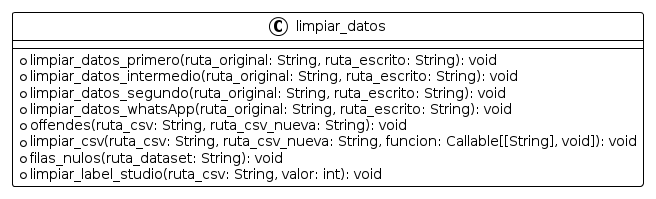
\includegraphics[width=0.65\textwidth]{capitulo5/figuras/fig1.png}
	\caption{Diagrama de clase del archivo limpiar\_datos
		\\\textit{Fuente: Elaboracion Propia}}
	\label{fig:uml1}
\end{figure}

\end{itemize}

%\textbf{Formato y Encadenamiento de Información}

La carpeta gestionarchivos contiene los archivos manejo\_archivos.py y convertir\_formato.py cada uno es importante para el uso de las funciones del archivo limpiar\_datos.py a continuacion se describen estos archivos:

\begin{itemize}

\item manejo\_archivos.py: Este archivo se encarga de la creación, copia, recorrido y vaciado de archivos en diferentes formatos. Para más detalles, consulte la figura \ref{fig:uml3}.

\begin{figure}[h!]
	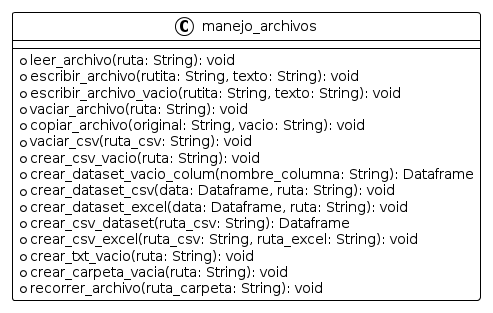
\includegraphics[width=0.65\textwidth]{capitulo5/figuras/fig3.png}
	\caption{Diagrama de clase del archivo manejo\_archivos
		\\\textit{Fuente: Elaboracion Propia}}
	\label{fig:uml3}
\end{figure}


\item convertir\_formato.py: Este archivo se ocupa de agrupar información de múltiples archivos para hacer uso de forma masiva de las funciones de limpieza definidas en el archivo limpiar\_datos.py, además de manejar el formato de los mismos cuando sea necesario. Para más detalles, consulte la figura \ref{fig:uml4}.

\begin{figure}[h!]
	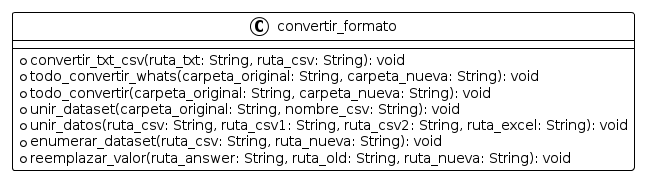
\includegraphics[width=0.8\textwidth]{capitulo5/figuras/fig4.png}
	\caption{Diagrama de clase del archivo convertir\_formato
		\\\textit{Fuente: Elaboracion Propia}}
	\label{fig:uml4}
\end{figure}

\end{itemize}

Es importante recordar que el preprocesamiento de datos varía según la fuente de los datos. Para más detalles sobre el proceso de limpieza de los datos provenientes de Facebook, consulte la figura \ref{fig:um12} (diagrama de actividades de Facebook) y el proceso de limpieza de datos provenientes de WhatsApp se puede apreciar en la figura \ref{fig:um13}(diagrama de actividades de Whatsapp).

\begin{figure}[h!]
	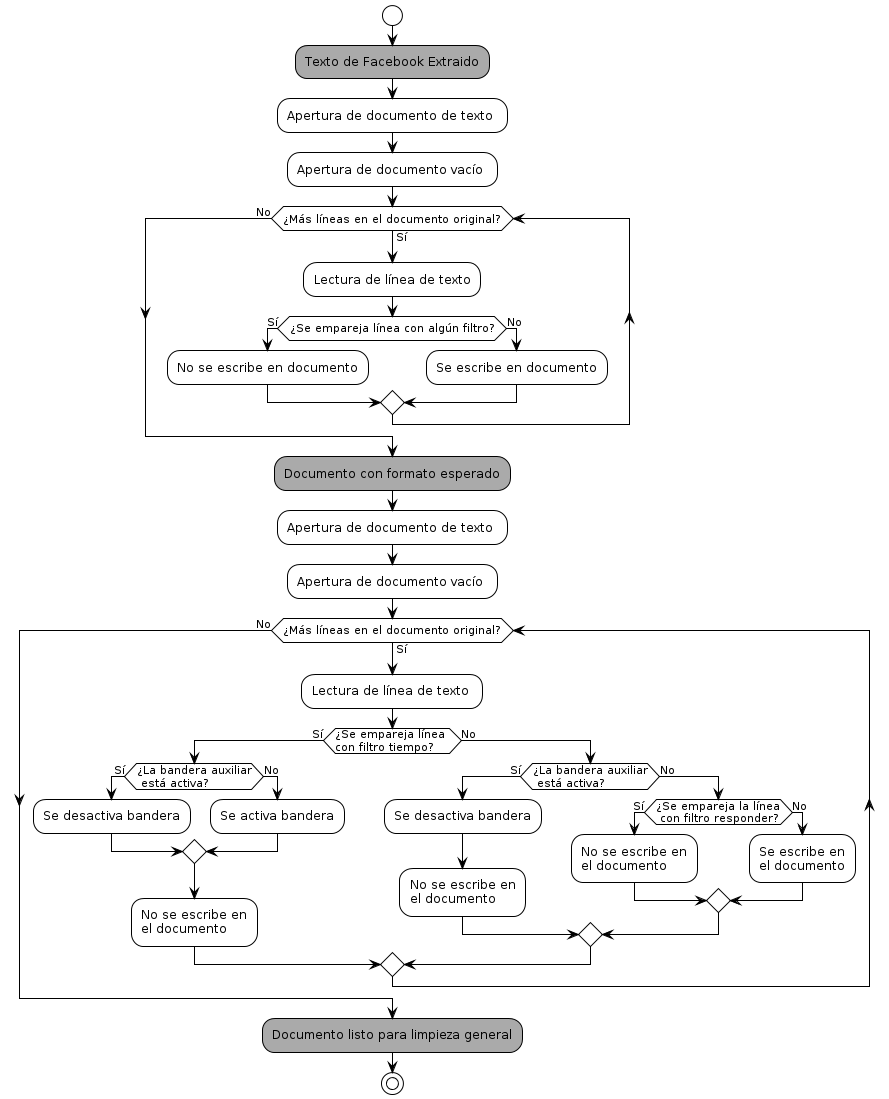
\includegraphics[width=1\textwidth]{capitulo5/figuras/prueba.png}
	\caption{Diagrama de actividades limpieza datos facebook
		\\\textit{Fuente: Elaboracion Propia}}
	\label{fig:um12}
\end{figure}

\begin{figure}[h!]
	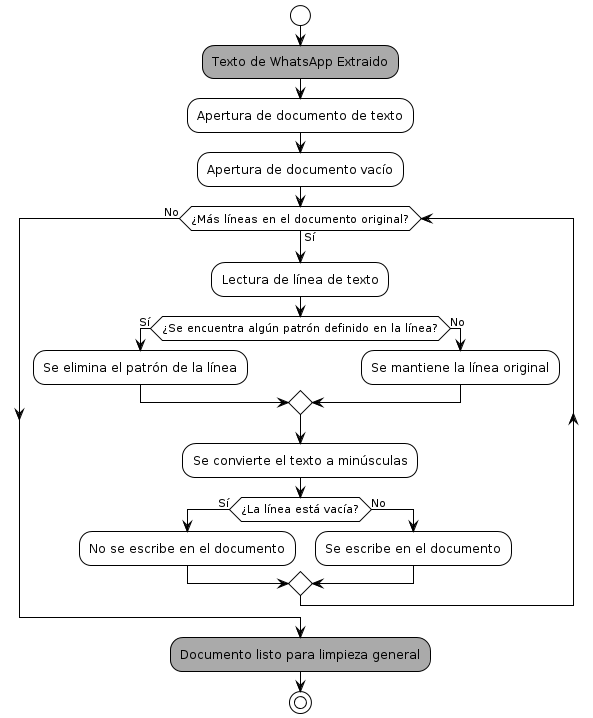
\includegraphics[width=0.7\textwidth]{capitulo5/figuras/part3.png}
	\caption{Diagrama de actividades limpieza datos whatsapp
		\\\textit{Fuente: Elaboracion Propia}}
	\label{fig:um13}
\end{figure}




\subsection{Implementación}
A continuación, se presenta el código fuente de los archivos detallados anteriormente en esta sección:

%\textbf{Limpieza de Datos}

%El archivo de la carpeta limpiezadataset se detalla a continuación:

El código fuente \ref{lst:c1} corresponde al archivo limpiar\_datos.py, donde se puede observar la implementación de la limpieza de datos extraídos de las redes sociales, se usaron expresiones regulares en la implementación de cada función. 

\lstinputlisting[language=Python,firstline=7,caption=Codigo fuente del archivo limpiar\_datos.py,label={lst:c1}]{capitulo5/codigo/limpiar_datos.py}

\vspace{-1.3em} % Ajusta el valor según sea necesario

\begin{figure}[h!]
	\centering % Incrementa el contador de lstlisting
	\textit{Fuente: Elaboración propia}
\end{figure}






La carpeta gestionarchivos almacena dos archivos y se enfoca en el tratamiento de archivos y formatos. En el código fuente \ref{lst:c3} se puede observar la implementación del archivo manejo\_archivos.py, que se encarga de crear, modificar, eliminar, y gestionar archivos en distintos formatos.

\lstinputlisting[language=Python,firstline=7,caption=Codigo fuente del archivo manejo\_archivos.py,label={lst:c3}]{capitulo5/codigo/manejo_archivos.py}
\vspace{-1.3em} % Ajusta el valor según sea necesario

\begin{figure}[h!]
	\centering % Incrementa el contador de lstlisting
	\textit{Fuente: Elaboración propia}
\end{figure}

En el código fuente \ref{lst:c4} se puede observar la implementación del último archivo de esta sección, convertir\_formato.py. Este archivo se encarga de recorrer múltiples archivos para compactar la información y realizar su conversión posterior. Además, se lleva a cabo el registro de cada archivo utilizado y de cada proceso realizado con este.

\lstinputlisting[language=Python,firstline=8,caption=Codigo fuente del archivo convertir\_formato.py,label={lst:c4}]{capitulo5/codigo/convertir_formato.py}
\vspace{-1.3em} % Ajusta el valor según sea necesario

\begin{figure}[h!]
	\centering % Incrementa el contador de lstlisting
	\textit{Fuente: Elaboración propia}
\end{figure}

\section{PREPROCESAMIENTO DE TEXTO}
En esta sección se detalla la implementación de cada paso realizado para el preprocesamiento de los datos, el cual se lleva a cabo después de la fase de limpieza de texto. En esta etapa, se trabaja con documentos de texto ya despojados de su formato original, facilitando su segmentación y tratamiento posterior. El objetivo principal del preprocesamiento es manejar la estructura interna del texto, segmentándolo en frases, oraciones o palabras, según sea más conveniente. El resultado de este proceso es un conjunto de datos limpio, útil y en uno de los formatos estándar aceptables para el uso del modelo de etiquetado. A continuación, se describe el archivo encargado del preprocesamiento de comentarios:

\begin{itemize}

\item corrector\_lenguaje.py: Este archivo aborda los aspectos generales de limpieza, que se pueden aplicar a varios tipos de información, independientemente de su fuente. Los detalles de este archivo se muestran en la figura \ref{fig:uml2}.

\begin{figure}[h!]
	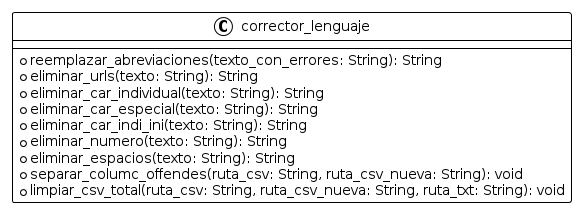
\includegraphics[width=0.65\textwidth]{capitulo5/figuras/fig2.png}
	\caption{Diagrama de clase del archivo corrector\_lenguaje
		\\\textit{Fuente: Elaboracion Propia}}
	\label{fig:uml2}
\end{figure}

\end{itemize}

La carpeta gestionarchivos contiene el archivo limpiar\_datos.py, que es utilizado en el archivo convertir\_formato.py. De manera similar, corrector\_lenguaje.py emplea el archivo manejo\_archivos.py, también ubicado en la misma carpeta. Esta organización permite que ambos archivos compartan la carpeta para aprovechar las funciones de tratamiento de formatos y la manipulación masiva de datos en múltiples archivos.
Una vez que los datos han pasado por los procesos de limpieza y preprocesamiento, se obtiene un producto final listo para ser utilizado en modelos de aprendizaje.



\subsection{Implementación}
A continuación, se presenta el código fuente del  archivo detallado anteriormente en esta sección:

El código fuente \ref{lst:c2} corresponde al archivo corrector\_lenguaje.py, que se encarga de la limpieza general de un conjunto de datos. Esto incluye la eliminación de URLs, caracteres especiales, números, entre otros elementos, utilizando la biblioteca re de Python.

\lstinputlisting[language=Python,firstline=7,caption=Codigo fuente del archivo corrector\_lenguaje.py,label={lst:c2}]{capitulo5/codigo/corrector_lenguaje.py}






\section{ETIQUETADO DE DATOS}
En este módulo se incluyen todos los pasos necesarios para el etiquetado de los datos adquiridos con el modelo BERT, su revisión y reetiquetado. El mismo contiene las siguientes secciones:

Etiquetado de Comentarios

La carpeta etiquetadodatos almacena los siguientes archivos:

\begin{itemize}

\item operacion\_dataset.py: Este archivo se encarga de diversas operaciones necesarias para el entrenamiento del modelo BERT, como la mezcla de datos, el conteo de clases y la división de conjuntos de datos. Para más detalles, consulte la figura 5.

------------------------------------------

figura 5

-----------------------------------------

\item bert\_multi.py: Este archivo se ocupa de la creación, configuración, entrenamiento y predicción, entre otras tareas específicas del modelo BERT. Para más detalles, consulte la figura 6.

---------------------------------------

figura 6

--------------------------------------

\end{itemize}

Reetiquetado y Revisión de Etiquetas

Para el reetiquetado de los conjuntos de datos, se utilizó la herramienta Label Studio, que acepta archivos en varios formatos como CSV y TSV. Esta herramienta proporciona una interfaz cómoda que agiliza el proceso de revisión, etiquetado y reetiquetado. Además, ofrece filtros y otras funciones que permiten realizar cambios en cualquier conjunto de datos, los cuales pueden exportarse en distintos formatos.



\subsection{Bert y el etiquetado de comentarios}
Durante la revisión del conjunto de datos ``Offendes'', se identificó que existian varias muestras que requerían reetiquetado, especialmente aquellas marcadas con lenguaje grosero. Por lo tanto, se revisó nuevamente todo el conjunto de datos, centrándose especialmente en las muestras con lenguaje grosero, y se procedió a reetiquetar manualmente teniendo en cuenta su utilidad y la percepción sobre si estos comentarios pertenecian a la categoria de groseros, ofensivos o no ofensivos en la sociedad boliviana.

De un total de 30,416 comentarios, 2,310 pertenecían a la clase de comentarios groseros pero no ofensivos. Se reetiquetaron 142 comentarios de esta clase y posteriormente se llevó a cabo la limpieza de este conjunto de datos para su uso adecuado.

El etiquetado de los conjuntos de datos de Facebook y WhatsApp se realizó después de la limpieza de los mismos. Para esta tarea, se utilizó la técnica de aprendizaje por transferencia, que consiste en aprovechar los conocimientos adquiridos en una tarea para mejorar el rendimiento en otra tarea relacionada pero diferente. En este caso, se empleó el dataset ``Offendes'' para afinar una versión reducida del modelo BERT, el cual fue inicialmente entrenado con grandes cantidades de texto no etiquetado, como páginas web, libros y artículos de noticias. A través de este proceso de entrenamiento masivo, el modelo aprende a comprender la estructura y el significado del lenguaje natural de manera general. Por lo tanto, cuando se adapta o afina para tareas específicas, como la clasificación de comentarios ofensivos, el modelo ya posee un conocimiento previo considerable del lenguaje, lo que permite mejorar su rendimiento en la tarea objetivo. Esto permitió que una muestra de aproximadamente 30,000 comentarios previamente etiquetados fuera utilizada para etiquetar los más de 78,000 comentarios recopilados de las redes sociales.

\begin{itemize}
 \item{Resultados del etiquetado con Bert}

Inicialmente, se utilizó el conjunto de datos ``Offendes'' para entrenar y afinar  el modelo BERT seleccionado, con el fin de etiquetar posteriormente el conjunto de datos recolectado de la región de los valles, centrándose específicamente en el departamento de Cochabamba. Los resultados del entrenamiento de BERT con ``Offendes'' se pueden apreciar en la Tabla \ref{tbl:bert}, donde en cantidad de muestras se detalla la cantidad de comentarios usados para el conjunto de entrenamiento, validación y prueba, en precisión la exactitud del modelo en su respectivo conjunto y en error las etiquetas que se marcaron incorrectamente en cada conjunto.

\begin{table}[!ht]
	\centering
	\begin{tabular}{|c|c|c|c|}
		\hline
		\textbf{Conjunto} & \textbf{Cantidad de muestras} & \textbf{Precisión} & \textbf{Error} \\ \hline
		Entrenamiento & 21169 & 0.9297 & 0.1969 \\ 
		Validación & 4536 & 0.8715 & 0.4100 \\ 
		Prueba & 4536 & 0.8748 & 0.3932 \\ \hline
		\textbf{Total} & 30241 & - & - \\ \hline
	\end{tabular}
	\caption{Resultados del entrenamiento de Bert con Offendes
		\\\textit{Fuente: Elaboración Propia}}
	\label{tbl:bert}
\end{table}


Bajo el resultado obtenido descrito en la Tabla \ref{tbl:bert}, se etiquetó el conjunto de datos de Cochabamba, cuyos resultados se detallan en la Tabla \ref{tbl:cochabamba}, donde la precisión es el resultado de la revisión manual realizada después del etiquetado. Finalmente despues de todo este proceso se etiquetaron los tres últimos conjuntos de datos restantes. En la tabla \ref{tbl:santacruz} se pueden observar los resultados del etiquetado del conjunto de datos de Santa Cruz, en la tabla \ref{tbl:lapaz} se presentan los resultados obtenidos para el conjunto de datos de La Paz, y finalmente, en la tabla \ref{tbl:whatsapp} se muestran los resultados obtenidos para el conjunto de datos de WhatsApp.


\begin{table}[!ht]
	\centering
	\begin{tabular}{|c|c|c|c|}
		\hline
		\textbf{Categorías} & \textbf{Cantidad} & \textbf{No de etiquetas cambiadas} & \textbf{Precisión (\%)} \\ \hline
		Ofensivos & 8199 & 3426 & 58.22 \\ 
		No ofensivos & 26856 & 1509 & 94.38 \\ 
		Groseros & 808 & 355 & 56.06 \\ \hline
		\textbf{Total} & 35863 & 5290 & \textbf{85.25} \\ \hline
	\end{tabular}
	\caption{Resultados del etiquetado de Bert para Cochabamba
		\\\textit{Fuente: Elaboración Propia}}
	\label{tbl:cochabamba}
\end{table}

\begin{table}[!ht]
	\centering
	\begin{tabular}{|c|c|c|}
		\hline
		\textbf{Categoría} & \textbf{Cantidad} & \textbf{Porcentaje (\%)} \\ \hline
		Ofensivo & 3171 & 22.33 \\ 
		No ofensivo & 10650 & 75.00 \\ 
		Grosero & 379 & 2.67 \\ \hline
		\textbf{Total} & 14200 & \textbf{100.00} \\ \hline
	\end{tabular}
	\caption{Resultados del etiquetado de Bert para Santa Cruz
		\\\textit{Fuente: Elaboración Propia}}
	\label{tbl:santacruz}
\end{table}


\begin{table}[!ht]
	\centering
	\begin{tabular}{|c|c|c|}
		\hline
		\textbf{Categoría} & \textbf{Cantidad} & \textbf{Porcentaje (\%)} \\ \hline
		Ofensivo & 4133 & 29.62 \\ 
		No ofensivo & 9379 & 67.18 \\ 
		Grosero & 449 & 3.21 \\ \hline
		\textbf{Total} & 13961 & \textbf{100.00} \\ \hline
	\end{tabular}
	\caption{Resultados del etiquetado de Bert para La Paz
		\\\textit{Fuente: Elaboración Propia}}
	\label{tbl:lapaz}
\end{table}

\begin{table}[!ht]
	\centering
	\begin{tabular}{|c|c|c|}
		\hline
		\textbf{Categoría} & \textbf{Cantidad} & \textbf{Porcentaje (\%)} \\ \hline
		Ofensivo & 2050 & 14.79 \\ 
		No ofensivo & 11129 & 80.31 \\ 
		Grosero & 680 & 4.90 \\ \hline
		\textbf{Total} & 13859 & \textbf{100.00} \\ \hline
	\end{tabular}
	\caption{Resultados del etiquetado de Bert para WhatsApp
		\\\textit{Fuente: Elaboración Propia}}
	\label{tbl:whatsapp}
\end{table}
\end{itemize}

\subsection{Implementación}
A continuación, se presenta el código fuente de cada archivo de la sección detallada:

%\textbf{Etiquetado de comentarios}

En la carpeta etiquetadodatos se almacenan dos archivos, el código fuente \ref{lst:c5} corresponde al archivo bert\_multi.py, donde se puede observar la implementación del modelo Bert y cualquier función necesaria para el guardado de datos y del modelo mismo.

\lstinputlisting[language=Python,firstline=11,caption=Codigo fuente del archivo bert\_multi.py,label={lst:c5}]{capitulo5/codigo/bert_multi.py}
\vspace{-1.3em} % Ajusta el valor según sea necesario

\begin{figure}[h!]
	\centering % Incrementa el contador de lstlisting
	\textit{Fuente: Elaboración propia}
\end{figure}

El código fuente \ref{lst:c6} corresponde al archivo operacion\_dataset.py, que contiene las funciones implementadas para las operaciones necesarias en los conjuntos de datos utilizados por el modelo BERT.


\lstinputlisting[language=Python,firstline=7,caption=Codigo fuente del archivo operacion\_dataset.py,label={lst:c6}]{capitulo5/codigo/operacion_dataset.py}
\vspace{-1.3em} % Ajusta el valor según sea necesario

\begin{figure}[h!]
	\centering % Incrementa el contador de lstlisting
	\textit{Fuente: Elaboración propia}
\end{figure}
\section{INGENIERÍA DE CARACTERÍSTICAS}
En esta sección se detallan los pasos para la división del conjunto de datos, cuyos elementos textuales serán posteriormente transformados en representaciones numéricas.

\subsection{División de comentarios}
Se trabajó con una porción del conjunto de datos total, específicamente con 35,000 muestras, las cuales se dividieron en tres partes: el conjunto de entrenamiento, el conjunto de prueba y el conjunto de validación. Las proporciones correspondientes a cada porción se pueden visualizar en la tabla \ref{tbl:conjuntos}, para asegurar la uniformidad en la distribución de clases, lo cual es crucial para el rendimiento del modelo, se creó este conjunto de datos priorizando una cantidad de muestras equilibrada para cada clase.


\begin{table}[!ht]
	\centering
	\begin{tabular}{|c|c|c|c|c|}
		\hline
		\textbf{Conjunto} & \textbf{Ofensivo} & \textbf{No ofensivo} & \textbf{Grosero} & \textbf{Porcentaje (\%)} \\ \hline
		Entrenamiento & 10250 & 10250 & 4000 & 24500 = 70\% \\ 
		Validación & 2125 & 2125 & 1000 & 5250 = 15\% \\ 
		Prueba & 2580 & 2572 & 98 & 5250 = 15\% \\ \hline
		\textbf{Total} & 14955 & 14947 & 5098 & \textbf{35.000 = 100\%} \\ \hline
	\end{tabular}
	\caption{División del conjunto de datos
		\\\textit{Fuente: Elaboración Propia}}
	\label{tbl:conjuntos}
\end{table}


Como se puede observar en la tabla \ref{tbl:conjuntos} la cantidad de clases en los conjuntos de datos no es uniforme para la categoría de lenguaje grosero, esto debido a que la cantidad de muestras totales para esta categoría no sobrepasa los 6000 ejemplares y por esa razón se priorizo otorgarle la mayor cantidad de muestras posibles a los conjuntos de entrenamiento y validación.
\subsection{Archivos de la representación textual}
A continuación, se detallan los diagramas de clases desarrollados para esta fase.

 La carpeta entrenarmodelos contiene cinco archivos, de los cuales dos son responsables de la división del conjunto de datos y su transformación en vectores numéricos densos, también conocidos como embeddings. Los archivos correspondientes son los siguientes: 

\begin{itemize}

\item creando\_dataset.py: Se encarga de la división de los conjuntos de datos en subconjuntos para el entrenamiento, la validación y la prueba, asegurando que cada una de las tres clases esté representada de la mejor manera para el entrenamiento de los modelos. También permite la visualización del estado del conjunto de datos, como el tamaño de secuencias y la bolsa de palabras, para mas detalles ver la figura \ref{fig:uml7}.

\begin{figure}
	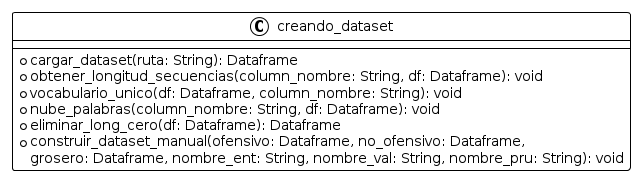
\includegraphics[width=0.65\textwidth]{capitulo5/figuras/fig7.png}
	\caption{Diagrama de clase del archivo creando\_dataset
		\\\textit{Fuente: Elaboración Propia}}
	\label{fig:uml7}
\end{figure}

\item preparar\_datos.py: Recibe el conjunto de datos en formato .CSV mismo que contiene comentarios textuales y sus etiquetas correspondientes. Convierte estos datos a listas para realizar procesos de tokenización, padding, carga de embeddings y procesamiento de embeddings, después de establecer los hiperparametros necesarios como el tamaño máximo de secuencia, el número máximo de palabras y la dimensión de los embeddings, además se crean métodos para el armado de la capa de embedding, compilación, entrenamiento, evaluación y graficación de los modelos, para mas detalles ver la figura \ref{fig:uml8}.

\begin{figure}[h!]
	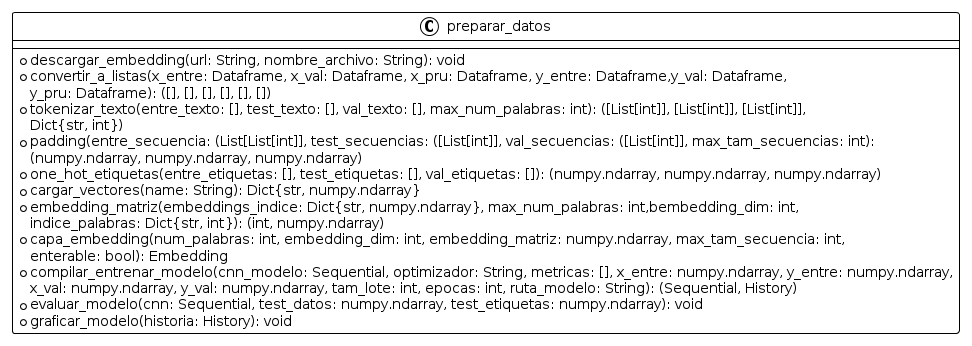
\includegraphics[width=0.95\textwidth]{capitulo5/figuras/fig8.png}
	\caption{Diagrama de clase del archivo preparar\_datos
		\\\textit{Fuente: Elaboración Propia}}
	\label{fig:uml8}
\end{figure}

\end{itemize}

Estos archivos abarcan los procesos de distribución equilibrada de clases, visualización de secuencias, conteo de palabras y creación de la bolsa de palabras del conjunto de datos final, además del manejo de los embeddings. Para la carga de embeddings, se utilizó la versión paga de Colab, debido a la necesidad de usar una mayor capacidad de memoria RAM.

\subsection{Implementación}
A continuación, se presenta el código fuente de los  archivos detallados anteriormente:

En el código fuente \ref{lst:c7} se puede observar la implementación del primer archivo, creando\_dataset.py, que visualiza el estado del conjunto de datos y lo divide manualmente, priorizando una distribución equilibrada entre las clases.

\lstinputlisting[language=Python,firstline=8,caption=Codigo fuente del archivo creando\_dataset.py,label={lst:c7}]{capitulo5/codigo/creando_dataset.py}

En el código fuente \ref{lst:c8} se observa la implementación del archivo preparar\_datos.py, que prepara la entrada final lista para la primera capa de los modelos propuestos. Esto implica la representación del texto en formas numéricas, en este caso, mediante embeddings. Además contiene funciones de armado, compilación, entrenamiento, entre otras funciones para los modelos de redes convolucionales

\lstinputlisting[language=Python,firstline=9,caption=Codigo fuente del archivo preparar\_datos,label={lst:c8}]{capitulo5/codigo/preparar_datos.py}

\section{MODELADO}
Se detallan los diferentes diagramas de clases de los restantes tres archivos de la carpeta entrenarmodelos, estos archivos contienen la implementación de los diversos modelos propuestos:

\begin{itemize}

\item cnn\_tres.py: Crea los modelos de redes convolucionales propuestos con una arquitectura base de tres capas, para más detalles ver la figura \ref{fig:uml9}.

\begin{figure}[h!]
	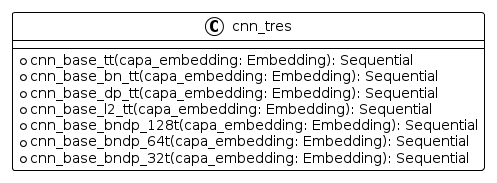
\includegraphics[width=0.65\textwidth]{capitulo5/figuras/fig9.png}
	\caption[Diagrama de clase del archivo cnn\_tres]{Diagrama de clase del archivo cnn\_tres
		\\\textit{Fuente: Elaboración Propia}}
	\label{fig:uml9}
\end{figure}

\item cnn\_four.py: Crea los modelos de redes convolucionales propuestos con una arquitectura base de cuatro capas, para más detalles ver la figura \ref{fig:uml10}.

\begin{figure}[h!]
	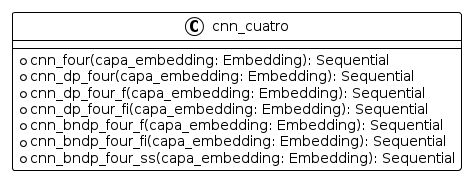
\includegraphics[width=0.6\textwidth]{capitulo5/figuras/fig10.png}
	\caption[Diagrama de clase del archivo cnn\_cuatro]{Diagrama de clase del archivo cnn\_cuatro
		\\\textit{Fuente: Elaboración Propia}}
	\label{fig:uml10}
\end{figure}

\item cnn\_dos.py: Crea los modelos de redes convolucionales propuestos con una arquitectura base de dos capas, para más detalles ver la figura \ref{fig:uml11}.

\begin{figure}[h!]
	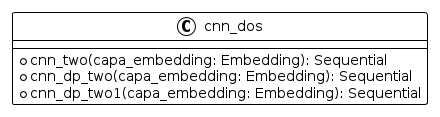
\includegraphics[width=0.5\textwidth]{capitulo5/figuras/fig11.png}
	\caption[Diagrama de clase del archivo cnn\_dos]{Diagrama de clase del archivo cnn\_dos
		\\\textit{Fuente: Elaboración Propia}}
	\label{fig:uml11}
\end{figure}

\end{itemize}

Para cada modelo propuesto, se guarda una copia en cualquier época durante el entrenamiento en la que la pérdida del conjunto de validación disminuya. Además, para mayor comodidad, se almacena todo el historial de entrenamiento de cada modelo, permitiendo visualizar su avance y realizar comparaciones con otros modelos.


\subsection{Implementación}
A continuación se detalla la implementación de cada archivo detallado en esta seccion:

En el código fuente \ref{lst:c9} se observa la implementación de todos los modelos de redes neuronales convolucionales basados en el modelo base propuesto, contenido en el archivo cnn\_tres.py.

\lstinputlisting[language=Python,firstline=7,caption=Codigo fuente del archivo cnn\_tres.py,label={lst:c9}]{capitulo5/codigo/cnn_tres.py}

En el código fuente \ref{lst:c10} se observa la implementación de los modelos propuestos con una capa convolucional mayor a la arquitectura base. Todo esto se encuentra en el archivo cnn\_cuatro.py

\lstinputlisting[language=Python,firstline=7,caption=Codigo fuente del archivo cnn\_cuatro.py,label={lst:c10}]{capitulo5/codigo/cnn_cuatro.py}

Finalmente, en el código fuente \ref{lst:c11} se observa la implementación de todos los modelos de redes neuronales convolucionales con dos capas, contenido en el archivo cnn\_dos.py.

\lstinputlisting[language=Python,firstline=7,caption=Codigo fuente del archivo cnn\_dos.py,label={lst:c11}]{capitulo5/codigo/cnn_dos.py}



\subsection{Desarrollo de los modelos convolucionales}
Para establecer la arquitectura base, los hiperparámetros y cualquier configuración necesaria en los modelos base, se aprovechó principalmente la teoría detallada en este proyecto, así como la documentación expuesta de las herramientas en uso, donde se pueden observar los valores que pueden establecerse. Además, se tuvieron en cuenta trabajos relacionados o similares a la tarea en cuestión. Se optó por utilizar una red neuronal convolucional 1D debido a la naturaleza de los datos textuales. Los hiperparámetros específicos se detallarán más adelante.

\begin{itemize}
	\item Hiperparametros de los modelos
\end{itemize}
Los hiperparámetros utilizados se pueden dividir en dos categorías. En la primera se encuentran los hiperparámetros constantes, que no se modificaron durante ni después de las pruebas, esta sección se enfocara en estos hiperparámetros. Respecto a la segunda categoria donde se trata a los hiperparámetros que se modificaron durante las pruebas se detallarán al momento de describir los modelos y sus resultados.

En la tabla \ref{tbl:3} se pueden observar los hiperparámetros utilizados para la capa de embedding en cada uno de los modelos convolucionales propuestos.

\begin{table}[!ht]
	\centering
	\begin{tabular}{|c|c|}
		\hline
		\textbf{Hiperparametro} & \textbf{Valor} \\ \hline
		max\_tam\_secuencia & 150 \\ \hline
		max\_num\_palabras  & 40000 \\ \hline
		embedding\_dim  & 300 \\ \hline
		max\_num\_palabras & 40000 \\ \hline
		embedding\_matriz & 30270 x 300 \\ \hline
		entrenable & False \\ \hline
	\end{tabular}
	\caption{Detalle Hiperparametros y valores usados para la capa de embedding
		\\\textit{Fuente: Elaboracion Propia}}
	\label{tbl:3}
\end{table}

Para las capas restantes, como las capas de convolución, se detallan los hiperparámetros constantes en la tabla \ref{tbl:4}.

\begin{table}[!ht]
	\centering
	\begin{tabular}{|c|c|}
		\hline
		\textbf{Hiperparametro } & \textbf{Valor} \\ \hline
		Optimizador & 'rmsprop' \\ \hline
		Batch\_size & 128 \\ \hline
		Epoca & 150 \\ \hline
		funcion\_activacion en capas convolucionales & 'relu' \\ \hline
		funcion\_activacion en capa densa intermedia & 'relu' \\ \hline
		funcion\_activacion en capa densa de salida & 'softmax' \\ \hline
	\end{tabular}
	\caption{Detalle Hiperparametros y valores usados para las capas restantes
		\\\textit{Fuente: Elaboracion Propia}}
	\label{tbl:4}
\end{table}

\begin{itemize}
	\item Primera iteración
\end{itemize}

En la primera iteración de las pruebas, se utilizó una red convolucional 1D con tres capas de convolución, dos capas de maxpooling, una capa de globalmaxpooling y dos capas densas. Esta arquitectura se puede observar con más detalle en la la tabla \ref{tbl:5}, la misma constituye la arquitectura base del modelo cnn\_base\_tt.


\begin{table}[!ht]
	\centering
	\begin{tabular}{|c|c|c|}
		\hline
		\textbf{Tipo de capa } & \textbf{Hiperparámetro } & \textbf{Valor} \\ \hline
		1ra capa convolucional 1D & num\_filtros, tam\_filtros, stride & 32, 3, 1 \\ \hline
		1ra capa maxpooling & tam\_pool, pool\_stride & 2, 2 \\ \hline
		2da capa convolucional 1D & num\_filtros, tam\_filtros, stride & 64, 5, 1 \\ \hline
		2da capa maxpooling & tam\_pool, pool\_stride & 2, 2 \\ \hline
		3ra capa convolucional 1D & num\_filtros, tam\_filtros, stride & 128, 5, 1 \\ \hline
		1ra capa densa intermedia & num\_neuronas & 128 \\ \hline
		2da capa densa de salida & num\_neuronas & 3 \\ \hline
	\end{tabular}
	\caption{Detalle arquitectura del modelo base
		\\\textit{Fuente: Elaboracion Propia}}
	\label{tbl:5}
\end{table}

De igual forma se detallan los modelos base utilizados junto con las técnicas de regularización aplicadas a cada uno. Se eligieron tres tipos de técnicas de regularización: normalización por lotes (batch normalization), regularización L2 y dropout. En esta iteración, se aplicó un tipo de regularización a cada capa convolucional. Los detalles  sobre cada uno de los modelos regularizados se presentan a continuación:

\begin{itemize}
	
	\item Modelo cnn\_base\_bn\_tt: Se aplicó normalización por lotes (batch normalization) a cada capa convolucional y a la capa densa intermedia, para más detalles ver la tabla \ref{tbl:cnn_base_bn_tt}.
	
	\begin{table}[!ht]
		\centering
		\begin{tabular}{|c|c|c|}
			\hline
			\textbf{Tipo de capa} & \textbf{Hiperparámetro} & \textbf{Valor} \\ \hline
			1ra capa convolucional 1D & num\_filtros, tam\_filtros, stride & 32, 3, 1 \\ \hline
			1ra capa BatchNormalization & - & - \\ \hline
			1ra capa maxpooling & tam\_pool, pool\_stride & 2, 2 \\ \hline
			2da capa convolucional 1D & num\_filtros, tam\_filtros, stride & 64, 5, 1 \\ \hline
			2da capa BatchNormalization & - & - \\ \hline
			2da capa maxpooling & tam\_pool, pool\_stride & 2, 2 \\ \hline
			3ra capa convolucional 1D & num\_filtros, tam\_filtros, stride & 128, 5, 1 \\ \hline
			3ra capa BatchNormalization & - & - \\ \hline
			1ra capa densa intermedia & num\_neuronas & 128 \\ \hline
			4ta capa BatchNormalization & - & - \\ \hline
			2da capa densa de salida & num\_neuronas & 3 \\ \hline
		\end{tabular}
		\caption{Arquitectura del modelo cnn\_base\_bn\_tt
			\\\textit{Fuente: Elaboracion Propia}}
		\label{tbl:cnn_base_bn_tt}
	\end{table}
	
	
	\item  Modelo cnn\_base\_dp\_tt: Se aplicó un dropout al 30\% a todas las capas convolucionales y un dropout al 50\% a la capa densa intermedia, para más detalles ver la tabla \ref{tbl:cnn_base_dp_tt}.
	
	\begin{table}[!ht]
		\centering
		\begin{tabular}{|c|c|c|}
			\hline
			\textbf{Tipo de capa} & \textbf{Hiperparámetro} & \textbf{Valor} \\ \hline
			1ra capa convolucional 1D & num\_filtros, tam\_filtros, stride & 32, 3, 1 \\ \hline
			1ra capa Dropout & tasa & 0.3 \\ \hline
			1ra capa maxpooling & tam\_pool, pool\_stride & 2, 2 \\ \hline
			2da capa convolucional 1D & num\_filtros, tam\_filtros, stride & 64, 5, 1 \\ \hline
			2da capa Dropout & tasa & 0.3 \\ \hline
			2da capa maxpooling & tam\_pool, pool\_stride & 2, 2 \\ \hline
			3ra capa convolucional 1D & num\_filtros, tam\_filtros, stride & 128, 5, 1 \\ \hline
			3ra capa Dropout & tasa & 0.3 \\ \hline
			1ra capa densa intermedia & num\_neuronas & 128 \\ \hline
			4ta capa Dropout & tasa & 0.5 \\ \hline
			2da capa densa de salida & num\_neuronas & 3 \\ \hline
		\end{tabular}
		\caption{Arquitectura del modelo cnn\_base\_dp\_tt
			\\\textit{Fuente: Elaboracion Propia}}
		\label{tbl:cnn_base_dp_tt}
	\end{table}
	
	
	\item  Modelo cnn\_base\_l2\_tt: Se aplicó regularización L2 con un valor de 0,05 a cada capa convolucional y a la capa densa intermedia, para más detalles ver la tabla \ref{tbl:cnn_base_l2_tt}.
	
	\begin{table}[!ht]
		\centering
		\begin{tabular}{|c|c|c|}
			\hline
			\textbf{Tipo de capa} & \textbf{Hiperparámetro} & \textbf{Valor} \\ \hline
			1ra capa convolucional 1D & num\_filtros, tam\_filtros, stride, L2 & 32, 3, 1, 0.05 \\ \hline
			1ra capa maxpooling & tam\_pool, pool\_stride & 2, 2 \\ \hline
			2da capa convolucional 1D & num\_filtros, tam\_filtros, stride, L2 & 64, 5, 1, 0.05 \\ \hline
			2da capa maxpooling & tam\_pool, pool\_stride & 2, 2 \\ \hline
			3ra capa convolucional 1D & num\_filtros, tam\_filtros, stride, L2 & 128, 5, 1, 0.05 \\ \hline
			1ra capa densa intermedia & num\_neuronas, L2 & 128, 0.05 \\ \hline
			2da capa densa de salida & num\_neuronas & 3 \\ \hline
		\end{tabular}
		\caption{Arquitectura del modelo cnn\_base\_l2\_tt
			\\\textit{Fuente: Elaboracion Propia}}
		\label{tbl:cnn_base_l2_tt}
	\end{table}
	
	
\end{itemize}

También se utilizaron modelos base con dos técnicas de regularización simultáneamente. Se mantuvieron las mismas características en cuanto a la arquitectura, pero se modificó la capa densa intermedia a 64 y 32 neuronas. A continuación, se detallan estos modelos:

\begin{itemize}
	
	\item Modelo cnn\_base\_bndp\_128tt: Se aplicó normalización por lotes (batch normalization) y dropout a cada capa convolucional y a la capa densa intermedia, para más detalles ver la tabla \ref{tbl:cnn_base_bndp_128tt}.
	
	\begin{table}[!ht]
		\centering
		\begin{tabular}{|c|c|c|}
			\hline
			\textbf{Tipo de capa} & \textbf{Hiperparámetro} & \textbf{Valor} \\ \hline
			1ra capa convolucional 1D & num\_filtros, tam\_filtros, stride & 32, 3, 1 \\ \hline
			1ra capa BatchNormalization & - & - \\ \hline
			1ra capa Dropout & tasa & 0.3 \\ \hline
			1ra capa maxpooling & tam\_pool, pool\_stride & 2, 2 \\ \hline
			2da capa convolucional 1D & num\_filtros, tam\_filtros, stride & 64, 5, 1 \\ \hline
			2da capa BatchNormalization & - & - \\ \hline
			2da capa Dropout & tasa & 0.3 \\ \hline
			2da capa maxpooling & tam\_pool, pool\_stride & 2, 2 \\ \hline
			3ra capa convolucional 1D & num\_filtros, tam\_filtros, stride & 128, 5, 1 \\ \hline
			3ra capa BatchNormalization & - & - \\ \hline
			3ra capa Dropout & tasa & 0.3 \\ \hline
			1ra capa densa intermedia & num\_neuronas & 128 \\ \hline
			4ta capa Dropout & tasa & 0.5 \\ \hline
			2da capa densa de salida & num\_neuronas & 3 \\ \hline
		\end{tabular}
		\caption{Arquitectura del modelo cnn\_base\_bndp\_128tt
			\\\textit{Fuente: Elaboracion Propia}}
		\label{tbl:cnn_base_bndp_128tt}
	\end{table}
	
	
	\item Modelo cnn\_base\_bndp\_64tt: Se aplicó normalización por lotes (batch normalization) y dropout a cada capa convolucional y dropout a la primera capa densa intermedia donde se redujo la cantidad de neuronas a 64, para más detalles ver la tabla \ref{tbl:cnn_base_bndp_64tt}.
	
	\begin{table}[!ht]
		\centering
		\begin{tabular}{|c|c|c|}
			\hline
			\textbf{Tipo de capa} & \textbf{Hiperparámetro} & \textbf{Valor} \\ \hline
			1ra capa convolucional 1D & num\_filtros, tam\_filtros, stride & 32, 3, 1 \\ \hline
			1ra capa BatchNormalization & - & - \\ \hline
			1ra capa Dropout & tasa & 0.3 \\ \hline
			1ra capa maxpooling & tam\_pool, pool\_stride & 2, 2 \\ \hline
			2da capa convolucional 1D & num\_filtros, tam\_filtros, stride & 64, 5, 1 \\ \hline
			2da capa BatchNormalization & - & - \\ \hline
			2da capa Dropout & tasa & 0.3 \\ \hline
			2da capa maxpooling & tam\_pool, pool\_stride & 2, 2 \\ \hline
			3ra capa convolucional 1D & num\_filtros, tam\_filtros, stride & 128, 5, 1 \\ \hline
			3ra capa BatchNormalization & - & - \\ \hline
			3ra capa Dropout & tasa & 0.3 \\ \hline
			1ra capa densa intermedia & num\_neuronas & 64 \\ \hline
			4ta capa Dropout & tasa & 0.5 \\ \hline
			2da capa densa de salida & num\_neuronas & 3 \\ \hline
		\end{tabular}
		\caption{Arquitectura del modelo cnn\_base\_bndp\_64tt
			\\\textit{Fuente: Elaboracion Propia}}
		\label{tbl:cnn_base_bndp_64tt}
	\end{table}
	
	
	\item Modelo cnn\_base\_bndp\_32tt: Se aplicó normalización por lotes (batch normalization) y dropout a cada capa convolucional y dropout a la primera capa densa intermedia, donde se redujo la cantidad de neuronas a 32, para más detalles ver la tabla \ref{tbl:cnn_base_bndp_32tt}.
	
	\begin{table}[!ht]
		\centering
		\begin{tabular}{|c|c|c|}
			\hline
			\textbf{Tipo de capa} & \textbf{Hiperparámetro} & \textbf{Valor} \\ \hline
			1ra capa convolucional 1D & num\_filtros, tam\_filtros, stride & 32, 3, 1 \\ \hline
			1ra capa BatchNormalization & - & - \\ \hline
			1ra capa Dropout & tasa & 0.3 \\ \hline
			1ra capa maxpooling & tam\_pool, pool\_stride & 2, 2 \\ \hline
			2da capa convolucional 1D & num\_filtros, tam\_filtros, stride & 64, 5, 1 \\ \hline
			2da capa BatchNormalization & - & - \\ \hline
			2da capa Dropout & tasa & 0.3 \\ \hline
			2da capa maxpooling & tam\_pool, pool\_stride & 2, 2 \\ \hline
			3ra capa convolucional 1D & num\_filtros, tam\_filtros, stride & 128, 5, 1 \\ \hline
			3ra capa BatchNormalization & - & - \\ \hline
			3ra capa Dropout & tasa & 0.3 \\ \hline
			1ra capa densa intermedia & num\_neuronas & 32 \\ \hline
			4ta capa Dropout & tasa & 0.5 \\ \hline
			2da capa densa de salida & num\_neuronas & 3 \\ \hline
		\end{tabular}
		\caption{Arquitectura del modelo cnn\_base\_bndp\_32tt
			\\\textit{Fuente: Elaboracion Propia}}
		\label{tbl:cnn_base_bndp_32tt}
	\end{table}
	
	
\end{itemize}

\begin{itemize}
	\item Segunda iteración
\end{itemize}

En esta iteración se realizaron cambios en la arquitectura de la red convolucional base, principalmente en la cantidad de capas de convolución y el pool\_stride. Los detalles de la arquitectura del modelo cnn\_four se encuentran en la tabla \ref{tbl:9}.

\begin{table}[!ht]
	\centering
	\begin{tabular}{|c|c|c|}
		\hline
		\textbf{Tipo de capa} & \textbf{Hiperparámetro} & \textbf{Valor} \\ \hline
		1ra capa convolucional 1D & num\_filtros, tam\_filtros, stride & 32, 3, 1 \\ \hline
		1ra capa maxpooling & tam\_pool, pool\_stride & 2, 1 \\ \hline
		2da capa convolucional 1D & num\_filtros, tam\_filtros, stride & 64, 5, 1 \\ \hline
		2da capa maxpooling & tam\_pool, pool\_stride & 2, 1 \\ \hline
		3ra capa convolucional 1D & num\_filtros, tam\_filtros, stride & 128, 5, 1 \\ \hline
		3ra capa maxpooling & tam\_pool, pool\_stride & 2, 1 \\ \hline
		4ra capa convolucional 1D & num\_filtros, tam\_filtros, stride & 256, 7, 1 \\ \hline
		1ra capa densa intermedia & num\_neuronas & 128 \\ \hline
		2da capa densa de salida & num\_neuronas & 3 \\ \hline
	\end{tabular}
	\caption{Detalle de la arquitectura de cuatro capas
	\\\textit{Fuente: Elaboracion Propia}}
	\label{tbl:9}
\end{table}

Todos los modelos propuestos a continuación comparten esta arquitectura base con métodos de regularización adicionales:

\begin{itemize}
	
	\item Modelo cnn\_dp\_four: Incluye dropout al 30\% después de cada capa convolucional y dropout al 50\% después de la capa densa intermedia, para más detalles ver tabla \ref{tbl:cnn_dp_four}.
	
	\begin{table}[!ht]
		\centering
		\begin{tabular}{|c|c|c|}
			\hline
			\textbf{Tipo de capa} & \textbf{Hiperparámetro} & \textbf{Valor} \\ \hline
			1ra capa convolucional 1D & num\_filtros, tam\_filtros, stride & 32, 3, 1 \\ \hline
			1ra capa Dropout & tasa & 0.3 \\ \hline
			1ra capa maxpooling & tam\_pool, pool\_stride & 2, 1 \\ \hline
			2da capa convolucional 1D & num\_filtros, tam\_filtros, stride & 64, 5, 1 \\ \hline
			2da capa Dropout & tasa & 0.3 \\ \hline
			2da capa maxpooling & tam\_pool, pool\_stride & 2, 1 \\ \hline
			3ra capa convolucional 1D & num\_filtros, tam\_filtros, stride & 128, 5, 1 \\ \hline
			3ra capa Dropout & tasa & 0.3 \\ \hline
			3ra capa maxpooling & tam\_pool, pool\_stride & 2, 1 \\ \hline
			4ta capa convolucional 1D & num\_filtros, tam\_filtros, stride & 256, 7, 1 \\ \hline
			4ta capa Dropout & tasa & 0.3 \\ \hline
			1ra capa densa intermedia & num\_neuronas & 128 \\ \hline
			5ta capa Dropout & tasa & 0.5 \\ \hline
			2da capa densa de salida & num\_neuronas & 3 \\ \hline
		\end{tabular}
		\caption{Arquitectura del modelo cnn\_dp\_four
			\\\textit{Fuente: Elaboracion Propia}}
		\label{tbl:cnn_dp_four}
	\end{table}
	
	
	\item Modelo cnn\_dp\_four\_f: Incluye dropout al 40\% después de cada capa convolucional y dropout al 50\% después de la capa densa intermedia, para más detalles ver la tabla \ref{tbl:cnn_dp_four_f}.
	
	\begin{table}[!ht]
		\centering
		\begin{tabular}{|c|c|c|}
			\hline
			\textbf{Tipo de capa} & \textbf{Hiperparámetro} & \textbf{Valor} \\ \hline
			1ra capa convolucional 1D & num\_filtros, tam\_filtros, stride & 32, 3, 1 \\ \hline
			1ra capa Dropout & tasa & 0.4 \\ \hline
			1ra capa maxpooling & tam\_pool, pool\_stride & 2, 1 \\ \hline
			2da capa convolucional 1D & num\_filtros, tam\_filtros, stride & 64, 5, 1 \\ \hline
			2da capa Dropout & tasa & 0.4 \\ \hline
			2da capa maxpooling & tam\_pool, pool\_stride & 2, 1 \\ \hline
			3ra capa convolucional 1D & num\_filtros, tam\_filtros, stride & 128, 5, 1 \\ \hline
			3ra capa Dropout & tasa & 0.4 \\ \hline
			3ra capa maxpooling & tam\_pool, pool\_stride & 2, 1 \\ \hline
			4ta capa convolucional 1D & num\_filtros, tam\_filtros, stride & 256, 7, 1 \\ \hline
			4ta capa Dropout & tasa & 0.4 \\ \hline
			1ra capa densa intermedia & num\_neuronas & 128 \\ \hline
			5ta capa Dropout & tasa & 0.5 \\ \hline
			2da capa densa de salida & num\_neuronas & 3 \\ \hline
		\end{tabular}
		\caption{Arquitectura del modelo cnn\_dp\_four\_f
			\\\textit{Fuente: Elaboracion Propia}}
		\label{tbl:cnn_dp_four_f}
	\end{table}
	
	
	\item Modelo cnn\_dp\_four\_fi: Incluye dropout al 50\% después de cada capa convolucional y después de la capa densa intermedia, para más detalles ver la tabla \ref{tbl:cnn_dp_four_fi}.
	
	\begin{table}[!ht]
		\centering
		\begin{tabular}{|c|c|c|}
			\hline
			\textbf{Tipo de capa} & \textbf{Hiperparámetro} & \textbf{Valor} \\ \hline
			1ra capa convolucional 1D & num\_filtros, tam\_filtros, stride & 32, 3, 1 \\ \hline
			1ra capa Dropout & tasa & 0.5 \\ \hline
			1ra capa maxpooling & tam\_pool, pool\_stride & 2, 1 \\ \hline
			2da capa convolucional 1D & num\_filtros, tam\_filtros, stride & 64, 5, 1 \\ \hline
			2da capa Dropout & tasa & 0.5 \\ \hline
			2da capa maxpooling & tam\_pool, pool\_stride & 2, 1 \\ \hline
			3ra capa convolucional 1D & num\_filtros, tam\_filtros, stride & 128, 5, 1 \\ \hline
			3ra capa Dropout & tasa & 0.5 \\ \hline
			3ra capa maxpooling & tam\_pool, pool\_stride & 2, 1 \\ \hline
			4ta capa convolucional 1D & num\_filtros, tam\_filtros, stride & 256, 7, 1 \\ \hline
			4ta capa Dropout & tasa & 0.5 \\ \hline
			1ra capa densa intermedia & num\_neuronas & 128 \\ \hline
			5ta capa Dropout & tasa & 0.5 \\ \hline
			2da capa densa de salida & num\_neuronas & 3 \\ \hline
		\end{tabular}
		\caption{Arquitectura del modelo cnn\_dp\_four\_fi
			\\\textit{Fuente: Elaboracion Propia}}
		\label{tbl:cnn_dp_four_fi}
	\end{table}
	
	
	\item Modelo cnn\_bndp\_four\_f: Incluye dropout al 40\% después de cada capa convolucional y dropout al 50\% después de la capa densa intermedia, más batch normalization en dos capas convolucionales, para más detalles ver la tabla \ref{tbl:cnn_bndp_four_f}.
	
	\begin{table}[!ht]
		\centering
		\begin{tabular}{|c|c|c|}
			\hline
			\textbf{Tipo de capa} & \textbf{Hiperparámetro} & \textbf{Valor} \\ \hline
			1ra capa convolucional 1D & num\_filtros, tam\_filtros, stride & 32, 3, 1 \\ \hline
			1ra capa BatchNormalization & - & - \\ \hline
			1ra capa Dropout & tasa & 0.5 \\ \hline
			1ra capa maxpooling & tam\_pool, pool\_stride & 2, 1 \\ \hline
			2da capa convolucional 1D & num\_filtros, tam\_filtros, stride & 64, 5, 1 \\ \hline
			2da capa Dropout & tasa & 0.5 \\ \hline
			2da capa maxpooling & tam\_pool, pool\_stride & 2, 1 \\ \hline
			3ra capa convolucional 1D & num\_filtros, tam\_filtros, stride & 128, 5, 1 \\ \hline
			3ra capa BatchNormalization & - & - \\ \hline
			3ra capa Dropout & tasa & 0.5 \\ \hline
			3ra capa maxpooling & tam\_pool, pool\_stride & 2, 1 \\ \hline
			4ta capa convolucional 1D & num\_filtros, tam\_filtros, stride & 256, 7, 1 \\ \hline
			4ta capa Dropout & tasa & 0.5 \\ \hline
			1ra capa densa intermedia & num\_neuronas & 128 \\ \hline
			5ta capa Dropout & tasa & 0.5 \\ \hline
			2da capa densa de salida & num\_neuronas & 3 \\ \hline
		\end{tabular}
		\caption{Arquitectura del modelo cnn\_bndp\_four\_f
			\\\textit{Fuente: Elaboracion Propia}}
		\label{tbl:cnn_bndp_four_f}
	\end{table}
	
	
	\item Modelo cnn\_bndp\_four\_fi: Incluye dropout al 50\% después de cada capa convolucional y dropout al 50\% después de la capa densa intermedia, más batch normalization en dos capas convolucionales, para más detalles ver la tabla \ref{tbl:cnn_bndp_four_fi}.
	
	\begin{table}[!ht]
		\centering
		\begin{tabular}{|c|c|c|}
			\hline
			\textbf{Tipo de capa} & \textbf{Hiperparámetro} & \textbf{Valor} \\ \hline
			1ra capa convolucional 1D & num\_filtros, tam\_filtros, stride & 32, 3, 1 \\ \hline
			1ra capa BatchNormalization & - & - \\ \hline
			1ra capa Dropout & tasa & 0.5 \\ \hline
			1ra capa maxpooling & tam\_pool, pool\_stride & 2, 1 \\ \hline
			2da capa convolucional 1D & num\_filtros, tam\_filtros, stride & 64, 5, 1 \\ \hline
			2da capa Dropout & tasa & 0.5 \\ \hline
			2da capa maxpooling & tam\_pool, pool\_stride & 2, 1 \\ \hline
			3ra capa convolucional 1D & num\_filtros, tam\_filtros, stride & 128, 5, 1 \\ \hline
			3ra capa BatchNormalization & - & - \\ \hline
			3ra capa Dropout & tasa & 0.5 \\ \hline
			3ra capa maxpooling & tam\_pool, pool\_stride & 2, 1 \\ \hline
			4ta capa convolucional 1D & num\_filtros, tam\_filtros, stride & 256, 7, 1 \\ \hline
			4ta capa Dropout & tasa & 0.5 \\ \hline
			1ra capa densa intermedia & num\_neuronas & 128 \\ \hline
			5ta capa Dropout & tasa & 0.5 \\ \hline
			2da capa densa de salida & num\_neuronas & 3 \\ \hline
		\end{tabular}
		\caption{Arquitectura del modelo cnn\_bndp\_four\_fi
			\\\textit{Fuente: Elaboracion Propia}}
		\label{tbl:cnn_bndp_four_fi}
	\end{table}
	
	
	\item Modelo cnn\_bndp\_four\_ss: Incluye dropout al 60\% después de cada capa convolucional y después de la capa densa intermedia, más batch normalization en cada capa convolucional, para más detalles ver la tabla \ref{tbl:cnn_bndp_four_ss}.
	
	\begin{table}[!ht]
		\centering
		\begin{tabular}{|c|c|c|}
			\hline
			\textbf{Tipo de capa} & \textbf{Hiperparámetro} & \textbf{Valor} \\ \hline
			1ra capa convolucional 1D & num\_filtros, tam\_filtros, stride & 32, 3, 1 \\ \hline
			1ra capa BatchNormalization & - & - \\ \hline
			1ra capa Dropout & tasa & 0.6 \\ \hline
			1ra capa maxpooling & tam\_pool, pool\_stride & 2, 1 \\ \hline
			2da capa convolucional 1D & num\_filtros, tam\_filtros, stride & 64, 5, 1 \\ \hline
			2da capa BatchNormalization & - & - \\ \hline
			2da capa Dropout & tasa & 0.6 \\ \hline
			2da capa maxpooling & tam\_pool, pool\_stride & 2, 1 \\ \hline
			3ra capa convolucional 1D & num\_filtros, tam\_filtros, stride & 128, 5, 1 \\ \hline
			3ra capa BatchNormalization & - & - \\ \hline
			3ra capa Dropout & tasa & 0.6 \\ \hline
			3ra capa maxpooling & tam\_pool, pool\_stride & 2, 1 \\ \hline
			4ta capa convolucional 1D & num\_filtros, tam\_filtros, stride & 256, 7, 1 \\ \hline
			4ta capa BatchNormalization & - & - \\ \hline
			4ta capa Dropout & tasa & 0.6 \\ \hline
			1ra capa densa intermedia & num\_neuronas & 128 \\ \hline
			5ta capa Dropout & tasa & 0.6 \\ \hline
			2da capa densa de salida & num\_neuronas & 3 \\ \hline
		\end{tabular}
		\caption{Arquitectura del modelo cnn\_bndp\_four\_ss
			\\\textit{Fuente: Elaboracion Propia}}
		\label{tbl:cnn_bndp_four_ss}
	\end{table}
	
	
\end{itemize}

\begin{itemize}
	\item Tercera iteración
\end{itemize}
Como última iteración, se experimentó con una red menos profunda de dos capas. La red convolucional cnn\_two se estableció como la arquitectura base, sus hiperparámetros y estructura se describen en la tabla \ref{tbl:11}.

\begin{table}[!ht]
	\centering
	\begin{tabular}{|c|c|c|}
		\hline
		\textbf{Tipo de capa} & \textbf{Hiperparámetro } & \textbf{Valor} \\ \hline
		1ra capa convolucional 1D & um\_filtros, tam\_filtros, stride & 64, 3, 1 \\ \hline
		1ra capa maxpooling & tam\_pool, pool\_stride & 2, 1 \\ \hline
		2da capa convolucional 1D & num\_filtros, tam\_filtros, stride & 128, 5, 1 \\ \hline
		1ra capa densa intermedia & num\_neuronas & 128 \\ \hline
		2da capa densa de salida & num\_neuronas & 3 \\ \hline
	\end{tabular}
	\caption{Detalle arquitectura de la red convolucional cnn\_two
		\\\textit{Fuente: Elaboracion Propia}}
	\label{tbl:11}
\end{table}

A partir de la arquitectura base del modelo cnn\_two, se añadieron técnicas de regularización dropout en los modelos propuestos a continuación:

\begin{itemize}
	
	\item Modelo cnn\_dp\_two: Se le aplicó un dropout del 30\% después de cada capa convolucional y un dropout del 50\% después de la capa densa intermedia, para más detalles ver la tabla \ref{tbl:cnn_dp_two}.
	
	\begin{table}[!ht]
		\centering
		\begin{tabular}{|c|c|c|}
			\hline
			\textbf{Tipo de capa} & \textbf{Hiperparámetro} & \textbf{Valor} \\ \hline
			1ra capa convolucional 1D & num\_filtros, tam\_filtros, stride & 64, 3, 1 \\ \hline
			1ra capa Dropout & tasa & 0.3 \\ \hline
			1ra capa maxpooling & tam\_pool, pool\_stride & 2, 1 \\ \hline
			2da capa convolucional 1D & num\_filtros, tam\_filtros, stride & 128, 5, 1 \\ \hline
			2da capa Dropout & tasa & 0.3 \\ \hline
			Capa densa intermedia & num\_neuronas & 128 \\ \hline
			3ra capa Dropout & tasa & 0.5 \\ \hline
			Capa densa de salida & num\_neuronas & 3 \\ \hline
		\end{tabular}
		\caption{Arquitectura del modelo cnn\_dp\_two
			\\\textit{Fuente: Elaboracion Propia}}
		\label{tbl:cnn_dp_two}
	\end{table}
	
	
	\item Modelo cnn\_dp\_two1: Se le aplicó un dropout del 10\% después de cada capa convolucional y un dropout del 20\% después de la capa densa intermedia, para más detalles ver la tabla \ref{tbl:cnn_dp_two1}.
	
	\begin{table}[!ht]
		\centering
		\begin{tabular}{|c|c|c|}
			\hline
			\textbf{Tipo de capa} & \textbf{Hiperparámetro} & \textbf{Valor} \\ \hline
			1ra capa convolucional 1D & num\_filtros, tam\_filtros, stride & 64, 3, 1 \\ \hline
			1ra capa Dropout & tasa & 0.1 \\ \hline
			1ra capa maxpooling & tam\_pool, pool\_stride & 2, 1 \\ \hline
			2da capa convolucional 1D & num\_filtros, tam\_filtros, stride & 128, 5, 1 \\ \hline
			2da capa Dropout & tasa & 0.1 \\ \hline
			Capa densa intermedia & num\_neuronas & 128 \\ \hline
			3ra capa Dropout & tasa & 0.2 \\ \hline
			Capa densa de salida & num\_neuronas & 3 \\ \hline
		\end{tabular}
		\caption{Arquitectura del modelo cnn\_dp\_two1
			\\\textit{Fuente: Elaboracion Propia}}
		\label{tbl:cnn_dp_two1}
	\end{table}
	
	
\end{itemize}

\clearpage

\section{EVALUACIÓN}
En esta sección se detalla la evaluación de todos los modelos propuestos según las métricas consideradas convenientes.
\subsection{Primera iteración}
Modelo Base

En la primera iteración de las pruebas, se utilizó una red convolucional 1D con tres capas de convolución, dos capas de maxpooling, una capa de globalmaxpooling y dos capas densas. Esta arquitectura se puede observar con más detalle en la figura 5.2. Los hiperparámetros base, como el numero de filtros, tamaño del stride, pool\_size, etc., se especifican en la tabla \ref{tbl:5}.

-----------------------------------------------------

figura 5.2

---------------------------------------------------

\begin{table}[!ht]
	\centering
	\begin{tabular}{|c|c|c|}
		\hline
		\textbf{Tipo de capa } & \textbf{Hiperparámetro } & \textbf{Valor} \\ \hline
		1ra capa convolucional 1D & num\_filtros, tam\_filtros, stride & 32, 3, 1 \\ \hline
		1ra capa maxpooling & tam\_pool, pool\_stride & 2, 2 \\ \hline
		2da capa convolucional 1D & num\_filtros, tam\_filtros, stride & 64, 5, 1 \\ \hline
		2da capa maxpooling & tam\_pool, pool\_stride & 2, 2 \\ \hline
		3ra capa convolucional 1D & num\_filtros, tam\_filtros, stride & 128, 5, 1 \\ \hline
		1ra capa densa intermedia & num\_neuronas & 128 \\ \hline
		2da capa densa de salida & num\_neuronas & 3 \\ \hline
	\end{tabular}
	\caption{Detalle arquitectura primera iteracion}
	\label{tbl:5}
\end{table}
  
En los resultados detallados en la figura algo1, se observa que el modelo sufre de sobreajuste. La precisión en el conjunto de entrenamiento aumenta constantemente a medida que avanzan las épocas, mientras que la precisión en el conjunto de validación disminuye. En la figura algo2, se muestra que el error en el conjunto de validación crece con el tiempo, mientras que el error en el conjunto de entrenamiento disminuye. Los resultados específicos se presentan en la tabla \ref{tbl:6}. Estos indicios sugieren la necesidad de utilizar técnicas de regularización para mitigar el sobreajuste.

---------------------------------------

figura algo 1

--------------------------------------

------------------------------------

figura algo 2

---------------------------------

\begin{table}[!ht]
	\centering
	\begin{tabular}{|c|c|c|c|c|c|}
		\hline
		\textbf{Nombre del modelo} & \textbf{Precisión} & \textbf{Perdida} & \textbf{Val\_Precisión} & \textbf{Val\_Perdida} & \textbf{Epoca} \\ \hline
		~ & 0.7522 & 0.59 & 0.7650 & 0.5743 & 3 \\ \cline{2-6} 
		cnn\_base\_tt & 0.978 & 0.04 & 0.7128 & 3.3866 & 109 \\ \cline{2-6} 
		~ & 0.9811 & 0.04 & 0.6893 & 3.8825 & 150 \\ \hline
	\end{tabular}
	\caption{Detalle resultados específicos primera iteracion}
	\label{tbl:6}
\end{table}

Modelo base y técnicas de regularización

A continuación, se detallan los modelos base utilizados junto con las técnicas de regularización aplicadas a cada uno. Se eligieron tres tipos de técnicas de regularización: normalización por lotes (batch normalization), regularización L2 y dropout. En esta iteración, se aplicó un tipo de regularización a cada capa convolucional. Los resultados obtenidos se presentan en la tabla \ref{tbl:7} y los detalles  sobre cada modelos a continuación:

\begin{itemize}
\item Modelo cnn\_base\_bn\_tt: Se aplicó normalización por lotes (batch normalization) a cada capa convolucional y a la capa densa intermedia.
\item Modelo cnn\_base\_dp\_tt: Se aplicó un dropout al 30\% a todas las capas convolucionales y un dropout al 50\% a la capa densa intermedia.
\item Modelo cnn\_base\_l2\_tt: Se aplicó regularización L2 con un valor de 0,05 a cada capa convolucional y a la capa densa intermedia.
\end{itemize}

\begin{table}[!ht]
	\centering
	\begin{tabular}{|c|c|c|c|c|c|}
		\hline
		\textbf{Nombre del modelo} & \textbf{Precisión} & \textbf{Perdida} & \textbf{Val\_Precisión} & \textbf{Val\_Perdida} & \textbf{Epoca} \\ \hline
		~ & 0.7890 & 0.52 & 0.7341 & 0.6090 & 4 \\ \cline{2-6} 
		cnn\_base\_bn\_tt & 0.9757 & 0.05 & 0.7272 & 2.8434 & 91 \\ \cline{2-6} 
		~ & 0.9800 & 0.04 & 0.5783 & 3.0617 & 150 \\ \hline
		~ & 0.7752 & 0.56 & 0.7646 & 0.5670 & 7 \\ \cline{2-6} 
		cnn\_base\_dp\_tt & 0.9000 & 0.25 & 0.7400 & 0.9013 & 133 \\ \cline{2-6} 
		~ & 0.9038 & 0.24 & 0.7274 & 0.8862 & 150 \\ \hline
		~ & 0.4185 & 1.02 & 0.4048 & 1.0484 & 123 \\ \cline{2-6} 
		cnn\_base\_l2\_tt & 0.4191 & 1.02 & 0.4048 & 1.0500 & 128 \\ \cline{2-6} 
		~ & 0.4118 & 1.02 & 0.4048 & 1.0503 & 150 \\ \hline
	\end{tabular}
	\caption{Detalle de los modelos base utilizados junto con las técnicas de regularización aplicadas}
	\label{tbl:7}
\end{table}

En los resultados detallados en la tabla \ref{tbl:7}, se observa que los métodos de regularización dropout y batch normalization (BN) retrasaron el sobreajuste. Sin embargo, al considerar el mejor modelo guardado con el menor error, el resultado es casi similar al obtenido por el modelo no regularizado. Por lo tanto, se probó el uso de dos técnicas de regularización simultáneamente en el modelo, manteniendo las mismas características pero modificando la capa densa intermedia a 64 y 32 neuronas en los modelos cnn\_base\_bndp\_64t y cnn\_base\_bndp\_32t, respectivamente. Los detalles y resultados se presentan en la tabla \ref{tbl:8}.

\begin{table}[!ht]
	\centering
	\begin{tabular}{|c|c|c|c|c|c|}
		\hline
		\textbf{Nombre del modelo} & \textbf{Precisión} & \textbf{Perdida} & \textbf{Val\_Precisión} & \textbf{Val\_Perdida} & \textbf{Epoca} \\ \hline
		~ & 0.8135 & 0.47 & 0.7596 & 0.5652 & 22 \\ \cline{2-6}
		cnn\_base\_bndp\_128t & 0.8967 & 0.26 & 0.7463 & 0.7757 & 126 \\ \cline{2-6}
		~ & 0.9029 & 0.25 & 0.7204 & 0.8861 & 150 \\ \hline
		~ & 0.7738 & 0.56 & 0.7777 & 0.5373 & 12 \\ \cline{2-6}
		cnn\_base\_bndp\_64t & 0.8701 & 0.34 & 0.7621 & 0.6211 & 65 \\ \cline{2-6}
		~ & 0.9058 & 0.25 & 0.7531 & 0.7155 & 150 \\ \hline
		~ & 0.8084 & 0.48 & 0.7804 & 0.5584 & 26 \\ \cline{2-6}
		cnn\_base\_bndp\_32t & 0.8580 & 0.37 & 0.7627 & 0.6342 & 56 \\ \cline{2-6}
		~ & 0.8962 & 0.28 & 0.7436 & 0.7562 & 150 \\ \hline
	\end{tabular}
	\caption{Detalle de los modelos base utilizados modificando la capa densa intermedia a 64 y 32 neuronas}
	\label{tbl:8}
\end{table}

Los resultados obtenidos en la tabla algo \ref{tbl;8} demuestran que, sin importar la época, el error en el conjunto de validación no sobrepasará 1.0 y siempre se mantendrá por debajo de ese rango. La precisión en el conjunto de validación se mantendrá siempre por encima de 0.75, siendo la mejor métrica de 0.78, obtenida por el modelo cnn\_base\_bndp\_32t, superando en 2 puntos la precisión del modelo base. Sin embargo, el modelo cnn\_base\_bndp\_64t fue el que obtuvo la menor pérdida.

\subsection{Segunda iteración}
En esta iteración se detallan los resultados obtenidos por los modelos con cuatro capas convolucionales, los detalles de la arquitectura base utilizada para cada modelo se especificaron anteriormente en la sección de modelado. 

Los resultados obtenidos en el modelo base, los modelos con una técnica de regularización y los modelos con dos técnicas de regularización se detallan en la tabla \ref{tbl:10}. Estos resultados no mostraron una mejora significativa en la precisión ni en la pérdida, por lo que se consideró innecesario desarrollar modelos más profundos. En su lugar, se decidió trabajar con un modelo menos profundo.


\begin{table}[!ht]
	\centering
	\begin{tabular}{|c|c|c|c|c|c|}
		\hline
		\textbf{Nombre del modelo} & \textbf{Precisión} & \textbf{Perdida} & \textbf{Val\_Precisión} & \textbf{Val\_Perdida} & \textbf{Epoca} \\ \hline
		~ & 0.7580 & 0.57 & 0.7714 & 0.5561 & 4 \\ \cline{2-6}
		cnn\_four & 0.8678 & 0.33 & 0.7206 & 0.8668 & 13 \\ \cline{2-6}
		~ & 0.9729 & 0.05 & 0.6937 & 4.4606 & 150 \\ \hline
		~ & 0.7870 & 0.53 & 0.7611 & 0.5810 & 11 \\ \cline{2-6}
		cnn\_dp\_four & 0.8528 & 0.37 & 0.7501 & 0.6475 & 41 \\ \cline{2-6}
		~ & 0.9019 & 0.25 & 0.7297 & 0.8340 & 150 \\ \hline
		~ & 0.8158 & 0.46 & 0.7650 & 0.5887 & 31 \\ \cline{2-6}
		cnn\_dp\_four\_f & 0.8665 & 0.35 & 0.7430 & 0.6575 & 108 \\ \cline{2-6}
		~ & 0.8726 & 0.33 & 0.7263 & 0.7339 & 150 \\ \hline
		~ & 0.8013 & 0.80 & 0.7699 & 0.5947 & 45 \\ \cline{2-6}
		cnn\_dp\_four\_fi & 0.8203 & 0.45 & 0.7625 & 0.6179 & 79 \\ \cline{2-6}
		~ & 0.8300 & 0.41 & 0.73 & 0.66 & 150 \\ \hline
		~ & 0.7611 & 0.59 & 0.7442 & 0.6174 & 19 \\ \cline{2-6}
		cnn\_bndp\_four\_f & 0.8096 & 0.48 & 0.7314 & 0.6467 & 42 \\ \cline{2-6}
		~ & 0.8662 & 0.34 & 0.5514 & 2.0138 & 150 \\ \hline
		~ & 0.7890 & 0.53 & 0.7650 & 0.5887 & 55 \\ \cline{2-6}
		cnn\_bndp\_four\_fi & 0.8021 & 0.49 & 0.7630 & 0.6190 & 74 \\ \cline{2-6}
		~ & 0.8345 & 0.41 & 0.7403 & 0.6992 & 150 \\ \hline
		~ & 0.7768 & 0.62 & 0.7255 & 0.5657 & 128 \\ \cline{2-6}
		cnn\_bndp\_four\_ss & 0.7849 & 0.54 & 0.7349 & 0.6329 & 141 \\ \cline{2-6}
		~ & 0.7832 & 0.54 & 0.7282 & 0.6471 & 150 \\ \hline
	\end{tabular}
	\caption{Detalle resultados obtenidos
		\\\textit{Fuente: Elaboracion Propia}}
	\label{tbl:10}
\end{table}

\subsection{Tercera iteración}
En esta sección se detallan los resultados del modelo base y  los modelos  base con una técnica de regularización con dos capas convolucionales, estos se muestran en  la tabla \ref{tbl:12}.

\begin{table}[!ht]
	\centering
	\begin{tabular}{|c|c|c|c|c|c|}
		\hline
		\textbf{Nombre del modelo} & \textbf{Precisión} & \textbf{Perdida} & \textbf{Val\_Precisión} & \textbf{Val\_Perdida} & \textbf{Epoca} \\ \hline
		cnn\_two & 0.7686 & 0.56 & 0.7787 & 0.5356 & 3 \\ \cline{2-6}
		~ & 0.9765 & 0.06 & 0.7004 & 2.2804 & 50 \\ \hline
		cnn\_dp\_two & 0.7747 & 0.55 & 0.7819 & 0.5524 & 8 \\ \cline{2-6}
		~ & 0.8718 & 0.32 & 0.7441 & 0.7408 & 50 \\ \hline
		cnn\_dp\_two1 & 0.7620 & 0.55 & 0.7746 & 0.5454 & 6 \\ \cline{2-6}
		~ & 0.9265 & 0.19 & 0.7303 & 1.0931 & 50 \\ \hline
	\end{tabular}
	\caption{Detalle resultados obtenidos}
	\label{tbl:12}
\end{table}




\subsection{Evaluación de los mejores modelos}
En esta sección se detallan los resultados obtenidos en el conjunto de prueba, el cual representa el 15\% de los datos del conjunto de datos total. Para esta tarea se seleccionaron los tres mejores modelos entrenados según la métrica de precisión global en el conjunto de validación. Además, como parte de una evaluación adicional, se emplearon los datos restantes del conjunto de datos recolectado junto con el conjunto de datos “offendes" para formar un nuevo conjunto de datos, este nuevo conjunto se evaluó con cada uno de los modelos seleccionados. Finalmente se presentaran más métricas de evaluación sobre el conjunto de prueba y el mejor modelo de red neuronal convolucional.

\begin{itemize}
\item Nuevo conjunto de prueba
\end{itemize}
Se creó un nuevo conjunto de datos utilizando las muestras restantes del conjunto total recolectado que no fueron utilizadas en el proceso de entrenamiento, validación y prueba de los modelos. Es importante destacar que la única categoría con datos extraídos exclusivamente de redes sociales bolivianas es la de ``lenguaje no ofensivo''. La categoría de ``lenguaje ofensivo'' es una combinación de datos extraídos tanto de redes sociales bolivianas como del conjunto de datos ``offendes''. Por otro lado, la categoría ``grosero'' está compuesta totalmente por datos generados por el modelo de lenguaje ChatGPT, es decir, son datos completamente nuevos.

Los detalles de este nuevo conjunto de datos se encuentran en la tabla \ref{tbl:categorias}, donde el número de muestras utilizadas del conjunto de datos extraído de las redes sociales bolivianas se denomina ``conjunto recolectado'', mientras que el número de muestras del conjunto ``offendes'' se denomina ``conjunto Offendes''.

\begin{table}[!ht]
	\centering
	\begin{tabular}{|c|c|c|c|c|}
		\hline
		\textbf{Categorías} & \textbf{Conjunto recolectado} & \textbf{Conjunto Offendes} & \textbf{Conjunto generado} & \textbf{Total} \\ \hline
		Ofensivos & 799 & 4201 & 0 & 5000 \\ \hline
		No ofensivos & 5000 & 0 & 0 & 5000 \\ \hline
		Groseros & 0 & 0 & 182 & 182 \\ \hline
		\textbf{Total} & 5799 & 4201 & 182 & 10182 \\ \hline
	\end{tabular}
	\caption{Distribución de categorías en el nuevo conjunto de datos
		\\\textit{Fuente: Elaboracion Propia}}
	\label{tbl:categorias}
\end{table}

\begin{itemize}
\item Desempeño con los conjuntos de prueba
\end{itemize}

A continuación se presentan los resultados obtenidos por los tres modelos seleccionados tanto en el conjunto de prueba original como en el conjunto de prueba nuevo. Los mismos se detallan en la tabla \ref{tbl:resultados}, y permiten evaluar la capacidad de generalización de cada modelo.


\begin{table}[!ht]
	\centering
	\begin{tabular}{|c|c|c|c|c|}
		\hline
		~ & \multicolumn{2}{|c|}{\textbf{Conjunto de prueba}} & \multicolumn{2}{|c|}{\textbf{Conjunto nuevo}} \\ \hline
		\textbf{Nombre del modelo} & \textbf{Precisión} & \textbf{Pérdida} & \textbf{Precisión} & \textbf{Pérdida} \\ \hline
		cnn\_base\_bndp\_32t & 0.7931 & 0.5348 & 0.5136 & 1.4332 \\ \hline
		cnn\_two & 0.7726 & 0.5524 & 0.5023 & 1.2967 \\ \hline
		cnn\_dp\_two & 0.7937 & 0.5205 & 0.5018 & 1.2430 \\ \hline
	\end{tabular}
	\caption{Resultados de los modelos en diferentes conjuntos
		\\\textit{Fuente: Elaboracion Propia}}
	\label{tbl:resultados}
\end{table}


En los resultados detallados en la tabla \ref{tbl:resultados}, se observa lo siguiente:

\begin{itemize}

\item El modelo cnn\_dp\_two demostró tener la mayor capacidad de generalización en el conjunto de datos de prueba bajo el contexto boliviano, ya que alcanzó la menor pérdida y la mayor precisión en comparación con los otros dos modelos.

\item En el conjunto de datos nuevo, que incluye principalmente las muestras recolectadas en contextos no bolivianos del conjunto de datos “offendes”, el modelo cnn\_base\_bndp\_32t exhibió la mejor capacidad de generalización, aunque sus resultados no difieren significativamente de los otros modelos. Para este conjunto de datos se observa una disminución en la precisión y un aumento en la pérdida, este fenómeno es completamente normal debido a las diferencias culturales y contextuales entre los conjuntos de datos.


\item Es importante destacar que la pérdida en el conjunto de datos de prueba bajo el contexto boliviano siempre se mantiene por debajo del 60\%. Además, la precisión de todos los modelos en este conjunto de datos siempre supera el 70\%.

\end{itemize}

\begin{itemize}
\item Evaluación del mejor modelo
\end{itemize}

A continuación se presentan los resultados de las métricas de precisión, sensibilidad y puntaje F1 del modelo cnn\_dp\_two para cada una de sus clases en el conjunto de datos de prueba bajo el contexto boliviano. Los detalles se encuentran en la tabla \ref{tbl:metrics}.

\begin{table}[!ht]
	\centering
	\begin{tabular}{|c|c|c|c|}
		\hline
		\textbf{Clase} & \textbf{Precisión} & \textbf{Sensibilidad} & \textbf{F1-Score} \\ \hline
		0 & 0.8269 & 0.8060 & 0.8163 \\ \hline
		1 & 0.7562 & 0.8181 & 0.7858 \\ \hline
		2 & 0.9082 & 0.3938 & 0.5480 \\ \hline
	\end{tabular}
	\caption{Métricas de rendimiento por clase
		\\\textit{Fuente: Elaboracion Propia}}
	\label{tbl:metrics}
\end{table}


Los resultados de la matriz de confusión para el modelo cnn\_dp\_two1 se pueden consultar en la imagen \ref{fig:matriz}.


\begin{figure}[!h]
	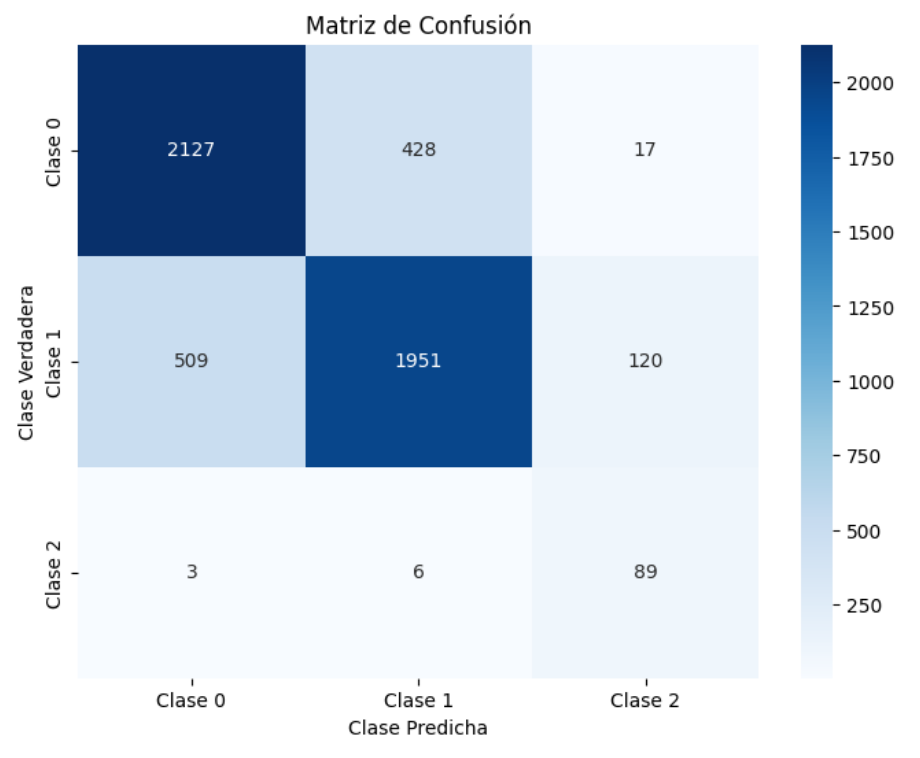
\includegraphics[width=0.8\textwidth]{capitulo5/figuras/matriz_confusion.PNG}
	\caption{Matriz de Confusión
		\\\textit{Fuente: Elaboracion Propia}}
	\label{fig:matriz}
\end{figure}

Los resultados de la matriz se pueden interpretar como:

\begin{itemize}

\item Clase 0:
Verdaderos Positivos (TP) = 2127
Falsos Negativos  (FN) = 428 + 17 = 445 (Ejemplos de clase 0 clasificados como 1 o 2)
Falsos Negativos Positivos (FP) = 509 + 3 = 512 (Ejemplos de clase 1 o 2 clasificados como 0)


\item Clase 1:
Verdaderos Positivos (TP) = 1951
Falsos Negativos (FN) = 509 + 120 = 629 (Ejemplos de clase 1 clasificados como 0 o 2)
Falsos Positivos (FP) = 428 + 6 = 434 (Ejemplos de clase 0 o 2 clasificados como 1)

\item Clase 2:
Verdaderos Positivos (TP) = 89
Falsos Negativos (FN) = 3 + 6 = 9 (Ejemplos de clase 2 clasificados como 0 o 1)
Falsos Positivos (FP) = 17 + 120 = 137 (Ejemplos de clase 0 o 1 clasificados como 2)

\end{itemize}

%\textbf{Análisis de las métricas de evaluación}

El análisis del desempeño del modelo cnn\_dp\_two revela los siguientes puntos importantes:

\begin{itemize}

\item Desempeño Desbalanceado:
El modelo muestra un buen desempeño en las Clases 0 y 1, con recall y precisión relativamente altos. 

\item Alta Precisión en Clase 2:
La Clase 2 muestra una alta precisión (aproximadamente 0.908), lo que indica que cuando el modelo predice la Clase 2, generalmente es correcto. Sin embargo, el bajo recall sugiere que no está detectando suficientes instancias de la Clase 2.

\item Falsos Positivos y Negativos:
Para la Clase 0 y la Clase 1, hay un número considerable de falsos positivos y falsos negativos. Esto sugiere que el modelo está confundiendo estas clases entre sí.


\end{itemize}


\section{DESPLIEGUE}
En esta sección se detalla la construcción de una aplicación de escritorio diseñada para la clasificación de comentarios textuales. Esta aplicación incluye la carga del mejor modelo previamente seleccionado, la matriz de embeddings y el tokenizador correspondiente. La misma permite al usuario ingresar un comentario que será procesado por el modelo clasificador, mostrando el resultado de la clasificación en la pantalla. Esta sección se compone de la siguiente carpeta:

La carpeta clasificadorcnn contiene los siguientes archivos:

\begin{itemize}

\item manipular\_modelo.py: Este archivo incluye funciones para cargar el tokenizador, la matriz de embeddings, ensamblar el modelo clasificador y preprocesar la entrada para realizar la predicción, para más detalles ver la figura \ref{fig:uml12}.

\begin{figure}[h!]
	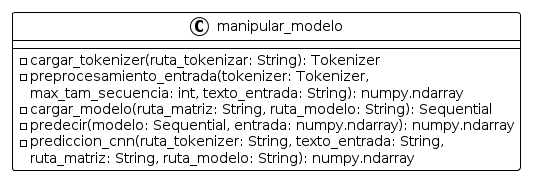
\includegraphics[width=0.8\textwidth]{capitulo5/figuras/fig12.png}
	\caption{Diagrama de clase del archivo manipular\_modelo.py
		\\\textit{Fuente: Elaboracion Propia}}
	\label{fig:uml12}
\end{figure}

\item interfaz.py: Este archivo se encarga de crear la interfaz de usuario, donde se ingresa el comentario a clasificar y se muestran los resultados de la clasificación, para más detalles ver la figura \ref{fig:uml13}.

\begin{figure}[h!]
	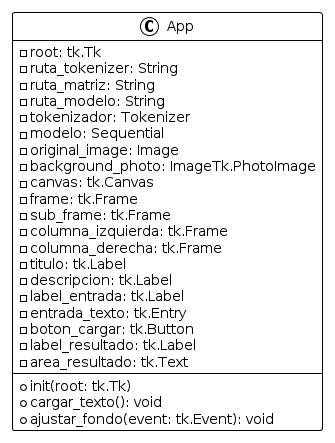
\includegraphics[width=0.5\textwidth]{capitulo5/figuras/fig13.png}
	\caption{Diagrama de clase del archivo interfaz.py
		\\\textit{Fuente: Elaboracion Propia}}
	\label{fig:uml13}
\end{figure}

\end{itemize}

Para simplificar la carga del modelo y hacer que los archivos sean más portables, se descompuso el modelo en varias partes:

\begin{itemize}

\item Matriz de embeddings: Se guardó en formato .npy, que es el formato nativo de la librería NumPy de Python, ampliamente utilizada en ciencia de datos y aprendizaje automático para cálculos numéricos. Este formato permite almacenar la matriz de manera eficiente y facilita su carga y uso posterior.

\item Pesos del modelo: Se almacenaron en formato .h5 (HDF5, Hierarchical Data Format version 5), un formato comúnmente usado para manejar datos de alta dimensión y ofrecer almacenamiento jerárquico. Esto permite reutilizar el modelo entrenado sin necesidad de volver a entrenarlo, ya que los pesos se pueden cargar directamente desde el archivo.

\item Tokenizador: Se guardó en formato .pickle, que es un formato binario utilizado en Python para la serialización y deserialización de objetos. Este formato es ideal para almacenar objetos complejos como los tokenizadores, que se usan en aplicaciones de procesamiento de lenguaje natural. La capacidad de .pickle para serializar prácticamente cualquier objeto Python, incluyendo listas, diccionarios y clases personalizadas, hace que sea una opción conveniente para este propósito.

\end{itemize}


\subsection{Implementación}
A continuación, se presenta el código fuente de cada archivo mencionado en la sección:

El código fuente \ref{lst:modelo} corresponde al archivo manipular\_modelo.py, donde se puede apreciar la implementación del cargado del modelo, su respectiva capa embedding con keras y el tokenizador con el módulo pickle de python para el preprocesado del texto de entrada.

\lstinputlisting[language=Python,firstline=7,caption=Codigo fuente del archivo manipular\_modelo.py
\\\textit{Fuente: Elaboracion Propia},label={lst:modelo}]{capitulo5/codigo/manipular_modelo.py}


El código fuente del archivo interfaz.py se desarrolló utilizando la librería Tkinter para crear una interfaz gráfica de usuario. Dado que es un componente secundario, no se proporcionarán detalles adicionales de este archivo.
\section{RECURSOS COMPUTACIONALES}
La implementación de los módulos diseñados y detallados anteriormente se llevó a cabo en dos computadoras personales y un servicio en la nube con las siguientes características:

Computadora Personal 1

\begin{itemize}

\item Procesador: Intel Core i7 no especificado
\item Memoria RAM: no especificada
\item Sistema Operativo: Windows 10
\item Tarjeta Gráfica: No especificada

\end{itemize}

Computadora Personal 2

\begin{itemize}

\item Procesador: MacBook Pro (modelo específico no indicado)
\item Memoria RAM: No especificada
\item Sistema Operativo: macOS Monterey
\item Tarjeta Gráfica: No especificada

\end{itemize}

Servicio en la Nube

\begin{itemize}

\item Recurso de Hardware: Acceso a GPUs y TPUs de alta calidad (T4, A100, L4 y TPU v2)
\item Memoria RAM: Amplia capacidad
\item Tiempo de Ejecución: Prolongado, mayor a 12 horas de ejecución
\item Sistema Operativo: Linux personalizado

\end{itemize}

En las siguientes subsecciones se detallan las herramientas de software utilizadas y la implementación llevada a cabo para la clasificación de comentarios, etiquetado de comentarios, creación, entrenamiento y uso de los modelos generados en el proceso de prueba.

\subsection{Herramientas de Software}
El lenguaje de programación utilizado es Python, elegido por su sintaxis clara y fácil de leer, lo que permite centrarse más en la lógica del código y menos en los detalles sintácticos. Además, Python cuenta con una amplia variedad de bibliotecas y frameworks específicos para el aprendizaje automático y análisis de datos, tales como TensorFlow, Keras, PyTorch, Scikit-learn, Matplotlib, Seaborn y Pandas. Todas estas herramientas ofrecen funciones avanzadas que facilitan el desarrollo de proyectos en esta área, asi como BERT. El mismo es el modelo utilizado para el etiquetado de texto, y significa Bidirectional Encoder Representations from Transformers. Es un modelo de lenguaje preentrenado desarrollado por Google, tiene una arquitectura compuesta por múltiples capas de transformers, que son unidades básicas que procesan secuencias de entrada de manera bidireccional. Esto significa que el modelo puede capturar el contexto de una palabra en una oración teniendo en cuenta tanto las palabras que la preceden como las que la siguen, lo que lo hace extremadamente efectivo para una amplia gama de tareas de procesamiento del lenguaje natural. Esto se logra mediante el entrenamiento del modelo en dos tareas: 

\begin{itemize}
\item El modelado de lenguaje enmascarado (Masked Language Modeling, MLM) que ocurre durante el entrenamiento, donde BERT recibe una secuencia de palabras de entrada y algunas de estas palabras son enmascaradas aleatoriamente. La tarea del modelo es predecir qué palabra falta en cada lugar enmascarado, lo que obliga al modelo a comprender el contexto de las palabras en una oración para poder predecir la palabra enmascarada con precisión. Ver figura \ref{fig:nlp8}

\item Predicción de la siguiente oración: Además del MLM, BERT también se entrena en una tarea de predicción de la siguiente oración. Se le proporcionan dos oraciones y el modelo debe predecir si la segunda oración sigue a la primera en un contexto coherente o no.
\end{itemize}

\begin{figure}[h!]
	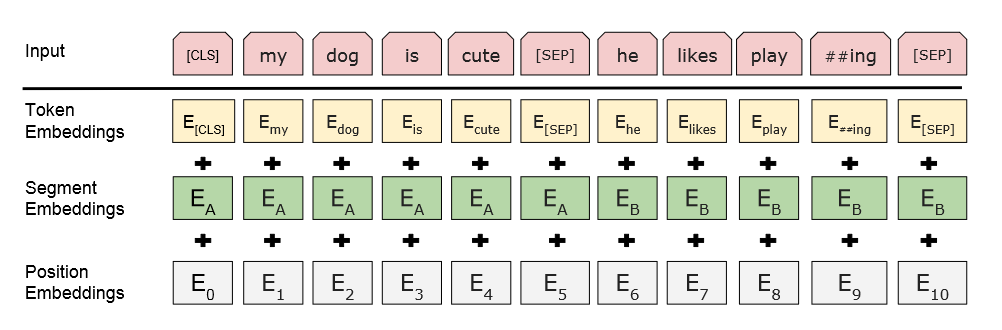
\includegraphics[width=0.65\textwidth]{capitulo3/figuras/nlp8.png}
	\caption[Representacion de entradas en BERT.]{Representacion de entradas en BERT.
		\\\textit{Fuente: Extraído de} \protect\cite[p. 5]{devlin2018bert} }
	\label{fig:nlp8}
\end{figure}

Para este proyecto, se utilizó la versión específica de BERT denominada ``bert\_uncased\_L-4\_H-512\_A-8'', una de las 24 variantes del conjunto ``BERT miniatura''. Estos modelos son versiones más compactas del BERT original, con una arquitectura reducida en comparación con BERT base o BERT grande, como se muestra en la tabla \ref{tbl:1}. Esto significa que tienen menos parámetros y requieren menos recursos computacionales para su entrenamiento y ejecución. Dado que los recursos necesarios para trabajar con un BERT base no están disponibles para este proyecto, utilizar este modelo compacto resultó extremadamente útil.

El modelo ``bert\_uncased\_L-4\_H-512\_A-8'' se entrena con texto en minúsculas, de ahí su denominación ``uncased''. Cuenta con cuatro capas (indicadas por ``L-4''), una dimensión de representación oculta de 512 en cada capa (indicada por ``H-512'') y utiliza ocho cabezas de atención en la capa de atención multi-cabeza (representadas por ``A-8'').

\begin{table}[!ht]
	\centering
	\caption[Representacion de versiones de BERT]{Representacion de versiones de BERT
		\\\textit{Fuente: Elaboracion Propia}}
	\begin{tabular}{|c|>{\centering\arraybackslash}m{2.5cm}|>{\centering\arraybackslash}m{2.5cm}|>{\centering\arraybackslash}m{3cm}|>{\centering\arraybackslash}m{2.5cm}|}
		\hline
		\textbf{} & \textbf{H=128} & \textbf{H=256} & \textbf{H=512} & \textbf{H=768} \\ \hline
		\textbf{L=2} & \makecell{2/128 \\ (BERT-Tiny)} & 2/256 & 2/512 & 2/768 \\ \hline
		\textbf{L=4} & 4/128 & \makecell{4/256 \\ (BERT-Mini)} & \makecell{4/512 \\ (BERT-Small)} & 4/768 \\ \hline
		\textbf{L=6} & 6/128 & 6/256 & 6/512 & 6/768 \\ \hline
		\textbf{L=8} & 8/128 & 8/256 & \makecell{8/512\\(BERT-Medium)} & 8/768 \\ \hline
		\textbf{L=10} & 10/128 & 10/256 & 10/512 & 10/768 \\ \hline
		\textbf{L=12} & 12/128 & 12/256 & 12/512 & \makecell{12/768 \\ (BERT-Base)} \\ \hline
	\end{tabular}
	\label{tbl:1}
\end{table}


Para cada tarea que se desee realizar con BERT, es crucial seleccionar los mejores hiperparámetros de ajuste a partir de las siguiente tabla \ref{tbl:2}:

\begin{table}[!ht]
	\centering
	\begin{tabular}{|c|c|}
		\hline
		\textbf{Hiperparametros} & \textbf{Valores} \\ \hline
		Tamaños de lote & 8, 16, 32, 64, 128 \\ \hline
		Tasas de aprendizaje & 3e-4, 1e-4, 5e-5, 3e-5 \\ \hline
		Número de épocas &  1, 2, 3, 4, 5 \\ \hline
		Tipo de capa de preprocesamiento & Según el modelo a usar \\ \hline
	\end{tabular}
	\caption[Detalle de hiperparametros y sus valores en BERT]{Detalle de hiperparametros y sus valores en BERT
		\\\textit{Fuente: Elaboracion Propia}}
	\label{tbl:2}
\end{table}

En este proyecto, para la tarea de etiquetado de los conjuntos de datos, se optó por un modelo de preprocesamiento ya entrenado específicamente seleccionado. La configuración específica incluyó:

\begin{itemize}

\item Capa de preprocesamiento: Una capa codificadora entrenable que se actualiza durante el entrenamiento(en-uncased-preprocess-version-3).
\item Capa de abandono: Con una tasa de abandono del 10\%.
\item Capa densa: Con una función de activación softmax para la clasificación múltiple.
\item Tamaño de lote: 32, lo que significa que los datos se dividen en lotes más pequeños con ese tamaño.
\item Tasa de aprendizaje: 3e-5.
\item Optimizador: AdamW.
\item Número de épocas: 5.

\end{itemize}

Para evaluar el modelo, se obtuvieron la pérdida y la precisión del modelo en el conjunto de prueba.

El entrenamiento del modelo BERT, el proceso de etiquetado de datos y la creación y entrenamiento de modelos de redes convolucionales se llevaron a cabo utilizando Google Colab (abreviatura de Colaboratory), una plataforma en línea proporcionada por Google. Colab permite escribir y ejecutar código Python en un entorno de cuaderno basado en la nube de forma gratuita como se muestra en la figura \ref{fig:bertito}. Está diseñado para facilitar la colaboración en proyectos de ciencia de datos y aprendizaje automático, así como para el desarrollo y experimentación con código Python sin necesidad de configurar un entorno local.

Google Colab ofrece acceso gratuito a recursos de cómputo en la nube, incluidas unidades de procesamiento gráfico (GPU) y unidades de procesamiento tensorial (TPU). Estos recursos fueron utilizados para el etiquetado de los conjuntos de datos. Sin embargo, el uso gratuito de CPU, GPU y TPU tiene limitaciones. Estas limitaciones se hicieron evidentes al entrenar el modelo BERT con grandes cantidades de datos, ya que el proceso requería mucho más tiempo de entrenamiento y el entorno se desconectaba, dejando el entrenamiento incompleto. Para evitar este problema, se adquirió el paquete Colab Pro, el cual garantiza que el entorno de ejecución no se desconecte y permite que BERT complete su entrenamiento sin interrupciones.

\begin{figure}[h!]
	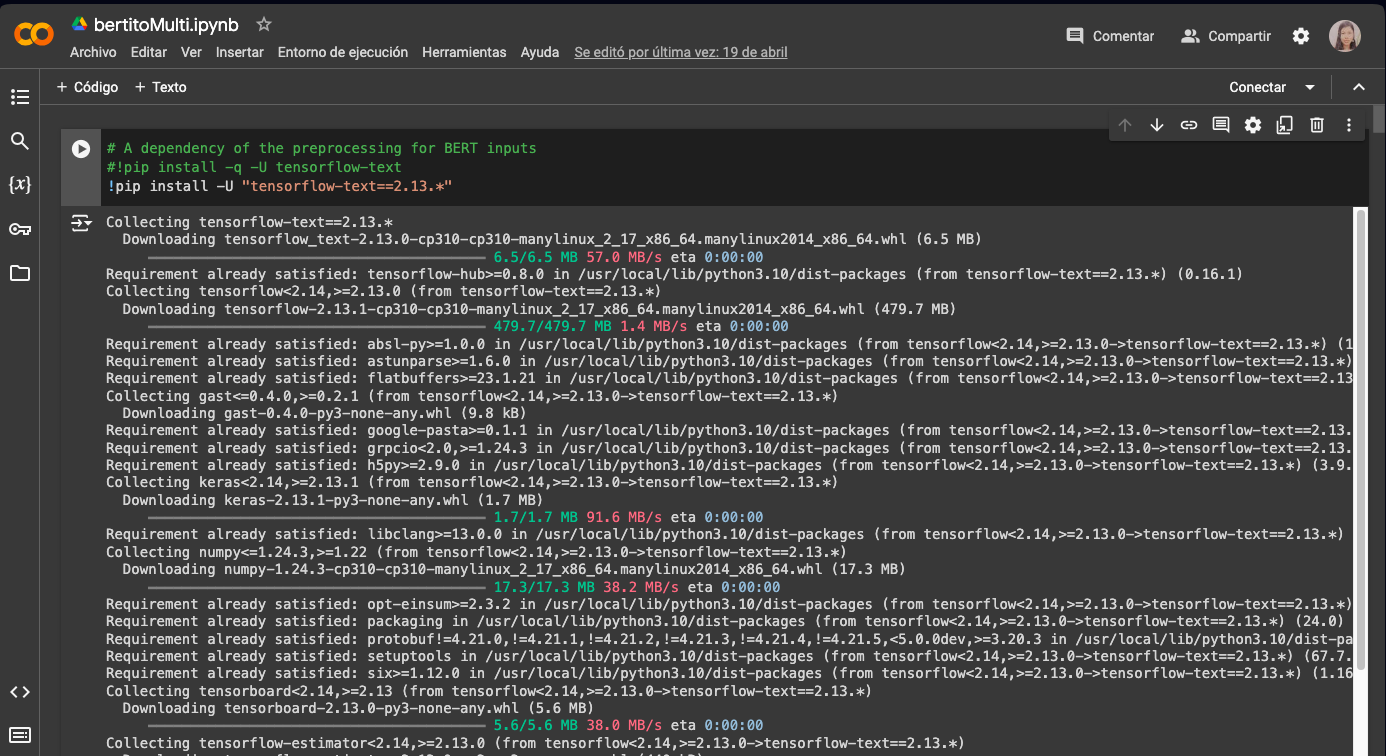
\includegraphics[width=1\textwidth]{capitulo5/figuras/bertito.png}
	\caption[Formato de cuaderno colab instalando libreria tensorflow-text-2.13]{Formato de cuaderno colab instalando libreria tensorflow-text-2.13
		\\\textit{Fuente: Elaboracion Propia}}
	\label{fig:bertito}
\end{figure}

Para la creación de los modelos de redes neuronales convolucionales se utilizó Keras, una API de alto nivel recomendada para TensorFlow a partir de su versión 1.14. Keras es una biblioteca de código abierto para la creación y entrenamiento de modelos de redes neuronales en Python. Es conocida por su facilidad de uso, ya que proporciona una interfaz de alto nivel que simplifica la construcción y el entrenamiento de modelos de redes neuronales. Los modelos de Keras se construyen utilizando capas que se pueden apilar o combinar de diversas formas para crear arquitecturas complejas.

A continuación, se detallan las versiones y bibliotecas utilizadas:

\begin{itemize}

\item Keras: 2.15.0
\item Matplotlib: 3.1.1
\item NumPy: 1.17.4
\item Python: 3.11.4
\item TensorFlow: 2.13.0 (para el modelo BERT)
\item Tensor-text: 2.13.0 (para el modelo BERT)
\item TensorFlow: 2.15.0 (para otros modelos)

\end{itemize}





\chapter{Conclusiones}\label{chp-conclusiones}







%



\backmatter

\renewcommand{\bibname}{Bibliografía} 

\bibliography{bibliografia/biblio.bib}
\bibliographystyle{apacite}
\clearpage
%\appendix
%\addcontentsline{toc}{section}{Apéndice}
%% !TEX root =../LibroTipoETSI.tex



%APENDICE A
\section*{Apéndice A}

\end{document}